\documentclass[oneside]{book}\usepackage[]{graphicx}\usepackage[dvipsnames,table,xcdraw]{xcolor}
% maxwidth is the original width if it is less than linewidth
% otherwise use linewidth (to make sure the graphics do not exceed the margin)
\makeatletter
\def\maxwidth{ %
  \ifdim\Gin@nat@width>\linewidth
    \linewidth
  \else
    \Gin@nat@width
  \fi
}
\makeatother

\definecolor{fgcolor}{rgb}{0.345, 0.345, 0.345}
\newcommand{\hlnum}[1]{\textcolor[rgb]{0.686,0.059,0.569}{#1}}%
\newcommand{\hlstr}[1]{\textcolor[rgb]{0.192,0.494,0.8}{#1}}%
\newcommand{\hlcom}[1]{\textcolor[rgb]{0.678,0.584,0.686}{\textit{#1}}}%
\newcommand{\hlopt}[1]{\textcolor[rgb]{0,0,0}{#1}}%
\newcommand{\hlstd}[1]{\textcolor[rgb]{0.345,0.345,0.345}{#1}}%
\newcommand{\hlkwa}[1]{\textcolor[rgb]{0.161,0.373,0.58}{\textbf{#1}}}%
\newcommand{\hlkwb}[1]{\textcolor[rgb]{0.69,0.353,0.396}{#1}}%
\newcommand{\hlkwc}[1]{\textcolor[rgb]{0.333,0.667,0.333}{#1}}%
\newcommand{\hlkwd}[1]{\textcolor[rgb]{0.737,0.353,0.396}{\textbf{#1}}}%
\let\hlipl\hlkwb

\usepackage{framed}
\makeatletter
\newenvironment{kframe}{%
 \def\at@end@of@kframe{}%
 \ifinner\ifhmode%
  \def\at@end@of@kframe{\end{minipage}}%
  \begin{minipage}{\columnwidth}%
 \fi\fi%
 \def\FrameCommand##1{\hskip\@totalleftmargin \hskip-\fboxsep
 \colorbox{shadecolor}{##1}\hskip-\fboxsep
     % There is no \\@totalrightmargin, so:
     \hskip-\linewidth \hskip-\@totalleftmargin \hskip\columnwidth}%
 \MakeFramed {\advance\hsize-\width
   \@totalleftmargin\z@ \linewidth\hsize
   \@setminipage}}%
 {\par\unskip\endMakeFramed%
 \at@end@of@kframe}
\makeatother

\definecolor{shadecolor}{rgb}{.97, .97, .97}
\definecolor{messagecolor}{rgb}{0, 0, 0}
\definecolor{warningcolor}{rgb}{1, 0, 1}
\definecolor{errorcolor}{rgb}{1, 0, 0}
\newenvironment{knitrout}{}{} % an empty environment to be redefined in TeX

\usepackage{alltt}
\usepackage[dvipsnames,table,xcdraw]{xcolor}

\usepackage{fontspec}
\setmainfont{XCharter}
\usepackage{anyfontsize}
\usepackage{microtype}
\usepackage[math-style=ISO,bold-style=ISO,warnings-off={mathtools-colon,mathtools-overbracket}]{unicode-math}

% -----------------------------------------------------------------------------

% CS 246
\usepackage{float}
\usepackage{listings}

\definecolor{light-gray}{gray}{0.95}
\newcommand{\code}[1]{\texttt{#1}}

% -----------------------------------------------------------------------------

% CO 250
\usepackage{tkz-berge}

% -----------------------------------------------------------------------------

% Core Packages
\usepackage{xfrac}
\usepackage[margin=1in]{geometry}
\usepackage[unicode,pdfversion=1.7]{hyperref}
\usepackage[shortlabels]{enumitem}
\usepackage[parfill]{parskip}
\usepackage[theorems,breakable]{tcolorbox}
\usepackage{graphicx}
\usepackage[ruled,linesnumbered,vlined,dotocloa]{algorithm2e}
\usepackage[delims=\lbrack\rbrack]{spalign}
\usepackage{mathtools}
\usepackage{cleveref}
\usepackage{pdfpages}
\usepackage{minted}
\usepackage{tikz}
\usetikzlibrary{patterns}
\usetikzlibrary{positioning}
\usepackage{pgfplots}
\pgfplotsset{compat=1.17}
\usepackage{framed}


% -----------------------------------------------------------------------------

% Better Tables
\usepackage{multicol}
\usepackage{booktabs}
\usepackage{adjustbox}
\usepackage{tabularx}
\newcolumntype{Y}{>{\centering\arraybackslash}X}
\newcolumntype{Z}{>{\centering\arraybackslash\columncolor{light-gray}}X}
\newcolumntype{B}{>{\centering\arraybackslash\bfseries}X}
\usepackage{multirow}
\usepackage[skip=1ex]{caption}

% -----------------------------------------------------------------------------

% Intervals
\usepackage{interval}
\intervalconfig{
    soft open fences,
    separator symbol={,}
}

% -----------------------------------------------------------------------------

\graphicspath{ {./figures/} }

\DeclareMathOperator{\rank}{rank}
\DeclareMathOperator{\slack}{slack}
\DeclareMathOperator{\row}{row}
\DeclareMathOperator{\cone}{cone}
\DeclareMathOperator{\nullspace}{Null}
\DeclareMathOperator{\ch}{char}
\DeclareMathOperator{\ord}{ord}
\DeclareMathOperator{\lcm}{lcm}

\usepackage{etoolbox}

% Functions
\providecommand\given{} % just to make sure it exists
\DeclarePairedDelimiterXPP{\E}[1]{\mathbb{E}}[]{}{
    \renewcommand\given{\nonscript\:\delimsize\vert\nonscript\:\mathopen{}}
    #1}
\DeclarePairedDelimiterXPP{\Var}[1]{\mathbb{V}}(){}{
    \renewcommand\given{\nonscript\:\delimsize\vert\nonscript\:\mathopen{}}
    #1}
\DeclarePairedDelimiterXPP\Prob[1]{\mathbb{P}}(){}{
    \renewcommand\given{\nonscript\:\delimsize\vert\nonscript\:\mathopen{}}
    \ifblank{#1}{\:\cdot\:}
    #1}
\DeclarePairedDelimiterXPP\Ind[1]{\mathbb{I}}\{\}{}{
\renewcommand\given{\nonscript\:\delimsize\vert\nonscript\:\mathopen{}}
\ifblank{#1}{\:\cdot\:}
#1}
\newcommand{\indep}{\perp\!\!\!\perp}
\DeclarePairedDelimiterXPP{\Corr}[1]{\text{Corr}}(){}{#1}
\DeclarePairedDelimiterXPP{\Cov}[1]{\text{Cov}}(){}{#1}
\DeclarePairedDelimiterXPP{\Sd}[1]{\text{Sd}}(){}{#1}
\DeclarePairedDelimiterXPP{\Se}[1]{\text{Se}}(){}{#1}
\let\SS=\relax
\DeclarePairedDelimiterXPP{\SS}[1]{\text{SS}}(){}{\text{#1}}
\DeclarePairedDelimiterXPP{\MS}[1]{\text{MS}}(){}{\text{#1}}
\DeclarePairedDelimiterXPP{\Span}[1]{\text{Span}}(){}{#1}
\DeclarePairedDelimiterXPP{\Spanc}[1]{\overline{\text{Span}}}(){}{#1}
\DeclareMathOperator{\VIF}{VIF}
\DeclarePairedDelimiterXPP{\expon}[1]{\text{exp}}\{\}{}{#1}

% Distributions
\DeclarePairedDelimiterXPP{\N}[1]{\mathcal{N}}(){}{#1}
\DeclarePairedDelimiterXPP{\uniform}[1]{\text{Uniform}}(){}{#1}
\DeclarePairedDelimiterXPP{\hyp}[1]{\text{Hypergeometric}}(){}{#1}
\DeclarePairedDelimiterXPP{\bern}[1]{\text{Bernoulli}}(){}{#1}
\DeclarePairedDelimiterXPP{\bin}[1]{\text{Binomial}}(){}{#1}
\DeclarePairedDelimiterXPP{\nb}[1]{\text{Negative Binomial}}(){}{#1}
\DeclarePairedDelimiterXPP{\geo}[1]{\text{Geometric}}(){}{#1}
\DeclarePairedDelimiterXPP{\poi}[1]{\text{Poisson}}(){}{#1}
\DeclarePairedDelimiterXPP{\mult}[1]{\text{Multinomial}}(){}{#1}
\DeclarePairedDelimiterXPP{\gam}[1]{\text{Gamma}}(){}{#1}
\DeclarePairedDelimiterXPP{\weib}[1]{\text{Weibull}}(){}{#1}
\DeclarePairedDelimiterXPP{\Mvn}[1]{\text{MVN}}(){}{#1}
\DeclarePairedDelimiterXPP{\Bvn}[1]{\text{BVN}}(){}{#1}
\DeclarePairedDelimiterXPP{\exponential}[1]{\text{Exponential}}(){}{#1}

\DeclarePairedDelimiterXPP{\tr}[1]{\text{trace}}(){}{#1}

\DeclarePairedDelimiterX\innerp[2]{\langle}{\rangle}{
    \ifblank{#1}{\:\cdot\:,}#1,
    \ifblank{#2}{\:\cdot\:}#2
}

\DeclarePairedDelimiterXPP{\MA}[1]{\text{MA}}(){}{#1}
\DeclarePairedDelimiterXPP{\AR}[1]{\text{AR}}(){}{#1}
\DeclarePairedDelimiterXPP{\ARMA}[1]{\text{ARMA}}(){}{#1}
\DeclarePairedDelimiterXPP{\AIC}[1]{\text{AIC}}(){}{#1}
\DeclarePairedDelimiterXPP{\BIC}[1]{\text{BIC}}(){}{#1}
\DeclarePairedDelimiterXPP{\ARIMA}[1]{\text{ARIMA}}(){}{#1}
\DeclarePairedDelimiterXPP{\GARCH}[1]{\text{GARCH}}(){}{#1}
\DeclarePairedDelimiterXPP{\NNAR}[1]{\text{NNAR}}(){}{#1}
\DeclarePairedDelimiterXPP{\NNSAR}[2]{\text{NNSAR}}(){_{#2}}{#1}
\DeclarePairedDelimiterXPP{\ARCH}[1]{\text{ARCH}}(){}{#1}

\DeclareMathOperator{\FWER}{FWER}
\let\log\relax
\DeclarePairedDelimiterXPP{\log}[1]{\text{log}}(){}{#1}

% -----------------------------------------------------------------------------

% Table of Contents
\hypersetup{colorlinks, linkcolor=[rgb]{0,0.5,1}}

% -----------------------------------------------------------------------------

% Heading Dates
\newcommand{\makeheading}[1]
{
    \begin{figure}[H]
        \centering
        \rule{\columnwidth}{1pt}\\
        {\large \scshape{#1}}\\[-0.6\baselineskip]
        \rule{\columnwidth}{1pt}
        \vspace*{-20pt}
    \end{figure}
}

% -----------------------------------------------------------------------------

% Definitions
\definecolor{myyellow}{RGB}{255,255,168}
% Theorems
\definecolor{mypurple}{RGB}{216,216,255}
% Algorithms
\definecolor{mygray}{RGB}{232,232,232}
% Examples
\definecolor{mygreen}{RGB}{216,255,216}
% Exercises
\definecolor{myred}{RGB}{255,216,216}
% Remarks
\definecolor{mycyan}{RGB}{204,229,229}

\tcbset{
    common/.style={
            fonttitle=\bfseries,
            coltitle=black,
            boxrule=0pt,
            breakable
        },
    theorem/.style={
            common,
            colback=mypurple,
            colframe=mypurple!95!black,
            fontupper=\itshape{}
        },
}


\newtcbtheorem[number within=section, crefname={definition}{definitions}]
{Definition}{DEFINITION}{
    common,
    colback=myyellow,
    colframe=myyellow!95!black
}{def}

\newtcbtheorem[use counter from=Definition, crefname={example}{examples}]
{Example}{EXAMPLE}{
    common,
    colback=mygreen,
    colframe=mygreen!95!black,
}{ex}

\newtcbtheorem[use counter from=Definition, crefname={exercise}{exercises}]
{Exercise}{EXERCISE}{
    common,
    colback=myred,
    colframe=myred!95!black,
}{exercise}

\newtcbtheorem[use counter from=Definition, crefname={remark}{remarks}]
{Remark}{REMARK}{
    common,
    colback=mycyan,
    colframe=mycyan!95!black,
}{remark}

\newtcbtheorem[use counter from=Definition, crefname={statistical Test}{statistical Tests}]
{Statistical_Test}{STATISTICAL TEST}{
    common,
    colback=Magenta!25!white,
    colframe=Magenta!50!white,
}{stest}

\newtcbtheorem[use counter from=Definition, crefname={theorem}{theorems}]
{Theorem}{THEOREM}{
    theorem
}{thm}

\newtcbtheorem[use counter from=Definition, crefname={proposition}{propositions}]
{Proposition}{PROPOSITION}{
    theorem
}{prop}

\newtcbtheorem[use counter from=Definition, crefname={corollary}{corollaries}]
{Corollary}{COROLLARY}{
    theorem
}{cor}

\newtcbtheorem[use counter from=Definition, crefname={lemma}{lemmas}]
{Lemma}{LEMMA}{
    theorem
}{lem}

\newtcbtheorem[no counter]
{Proof}{Proof of}{
    common,
    colframe=black!10,
    separator sign={}
}{pf}

\DeclarePairedDelimiterX\norm[1]\lVert\rVert{\ifblank{#1}{\:\cdot\:}{#1}}
\DeclarePairedDelimiterX\abs[1]\lvert\rvert{\ifblank{#1}{\:\cdot\:}{#1}}
\DeclarePairedDelimiter\set\{\}
\DeclareMathOperator*{\argmax}{arg\,max}
\DeclareMathOperator*{\argmin}{arg\,min}
\DeclareMathOperator*{\arginf}{arg\,inf}
\DeclareMathOperator*{\argsup}{arg\,sup}

% just to make sure it exists
\providecommand\onto{}
% can be useful to refer to this outside \Set
\newcommand\SetSymbol[1][]{%
    \nonscript\:#1\vert{}
    \allowbreak\nonscript\:
    \mathopen{}}
\DeclarePairedDelimiterXPP\Proj[1]{\text{Proj}}(){}{%
    \renewcommand\onto{\SetSymbol[\delimsize]}
    #1
}

\AtBeginDocument{%
    \let\mathbb\relax
    \DeclareMathAlphabet{\mathbb}{U}{msb}{m}{n}%
}

\newenvironment{tightcenter}{%
    \setlength\topsep{0pt}%
    \setlength\parskip{0pt}%
    \par\centering}{\par\noindent\ignorespacesafterend}

\usepackage{nicematrix}
\setcounter{secnumdepth}{3}
\setcounter{tocdepth}{3}
\usepackage{commath}

\title{
\LARGE Sampling and Experimental Design\\
\large STAT 332\\
\normalsize Winter 2021 (1211)}
\author{\LaTeX{}er: \emph{Cameron Roopnarine}\\Instructor: \emph{Riley Metzger}}
\date{\today}
\IfFileExists{upquote.sty}{\usepackage{upquote}}{}
\begin{document}

\maketitle

\tableofcontents



\chapter{Assignment 1}
\section{Lecture 1.00: PPDAC + Example}
PPDAC\@: \underline{P}roblem, \underline{P}lan, \underline{D}ata,
\underline{A}nalysis, \underline{C}onclusion.
\begin{enumerate}
    \item \underline{P}roblem: Define the problem.
          \begin{itemize}
              \item \textbf{Target population} (TP): The group of units referred to in the problem step.
              \item \textbf{Response}: The answer provided by the TP to the problem.
              \item \textbf{Attribute}: Statistic of the response.
                    \begin{Example}{}{}
                        What is the average grade of the students in STAT 101?
                        \begin{itemize}
                            \item Target population: All STAT 101 students
                            \item Response: Grade of a STAT 101 student.
                            \item Attribute: Average grade.
                        \end{itemize}
                    \end{Example}
          \end{itemize}
    \item \underline{P}lan: How exactly are you going to answer the problem you posed yourself?
          \begin{itemize}
              \item \textbf{Study population} (SP): The set of units you \emph{can} study.
                    The study population is not necessarily a subset of the target population.
                    \begin{Example}{}{}
                        Does a drug reduce hair loss?
                        \begin{itemize}
                            \item Target population: People.
                            \item Study population: Mice.
                        \end{itemize}
                        Note that mice is not a subset of people,
                        so the study population and target population are not subsets of one
                        another.
                    \end{Example}
              \item \textbf{Sample}: A subset of the study population.
                    In the prior example, it would be the set of mice you
                    select from your study population that are of interest
                    in the sample.
              \item \textbf{Data}: Collect the data, according to the plan.
          \end{itemize}
    \item \underline{A}nalysis: We analyze the data.
    \item \underline{C}onclusion: Refers back to the problem. We also
          note some common \emph{errors}.
          \begin{enumerate}
              \item \textbf{Study error}: The attribute of the population the
                    target population differs from the parameter of the study population.
                    \begin{Example}{}{}
                        Mathematically we can write it down as $ a(\text{TP})-\mu $,
                        however this error is qualitative. Therefore, we cannot
                        actually calculate it.
                    \end{Example}
              \item \textbf{Sample error}: The parameter differs from the
                    sample statistic, sometimes called an estimate.
                    \begin{Example}{}{}
                        Mathematically we can write it down as $ \mu-\bar{x} $,
                        however this error is qualitative. Therefore, we cannot
                        actually calculate it.
                    \end{Example}
              \item \textbf{Measurement error}: The difference
                    between what \emph{we want} to calculate and what \emph{we do}
                    calculate.
                    \begin{Example}{}{}
                        IQ is an interesting thing. You want to measure somebody's intelligence,
                        and yet if you go and actually calculate it, they're using various
                        statistical tests or various psychological tests
                        that could have a lot of measurement error.
                    \end{Example}
          \end{enumerate}
\end{enumerate}

\section{Lecture 2.00: Models, Model 1}
\begin{Definition}{Model}{}
    A \textbf{model} relates a study population parameter to a response.
\end{Definition}
\begin{Definition}{Model 1}{}
    \textbf{Model 1} is defined as
    \[ Y_j=\mu+R_j\quad\text{where $R_j\sim\N{0,\sigma^2}$} \]
    where
    \begin{itemize}
        \item $ Y_j $: random parameter that is the response of unit $ j $.
        \item $ \mu $: study population parameter. In this case, it's
              the mean and is non-random. However, it is unknown.
        \item $ R_j $: error term. It gives the distribution of
              responses about $ \mu $.
    \end{itemize}
\end{Definition}
\begin{figure}[!htbp]
    \centering
    \begin{tikzpicture}[x=0.75pt,y=0.75pt,yscale=-1,xscale=1]
        %uncomment if require: \path (0,100); %set diagram left start at 0, and has height of 100

        %Straight Lines [id:da9261923254109076] 
        \draw    (1,48) -- (151,48) ;
        %Straight Lines [id:da2635399060635354] 
        \draw    (12,5) -- (12,85) ;
        %Shape: Circle [id:dp9095100382272178] 
        \draw  [fill={rgb, 255:red, 0; green, 0; blue, 0 }  ,fill opacity=1 ] (49.9,68.05) .. controls (49.9,66.37) and (51.27,65) .. (52.95,65) .. controls (54.63,65) and (56,66.37) .. (56,68.05) .. controls (56,69.73) and (54.63,71.1) .. (52.95,71.1) .. controls (51.27,71.1) and (49.9,69.73) .. (49.9,68.05) -- cycle ;
        %Shape: Brace [id:dp37424480000501614] 
        \draw   (49.8,49.1) .. controls (47.19,48.96) and (45.82,50.2) .. (45.68,52.81) -- (45.68,52.81) .. controls (45.49,56.53) and (44.09,58.32) .. (41.48,58.19) .. controls (44.09,58.32) and (45.29,60.25) .. (45.09,63.98)(45.18,62.31) -- (45.09,63.98) .. controls (44.96,66.59) and (46.19,67.96) .. (48.8,68.1) ;

        % Text Node
        \draw (153,48) node [anchor=west] [inner sep=0.75pt]    {$\mu $};
        % Text Node
        \draw (23,52.4) node [anchor=north west][inner sep=0.75pt]    {$R_{j}$};
        % Text Node
        \draw (54.95,71.45) node [anchor=north west][inner sep=0.75pt]    {$y_{j}$};
    \end{tikzpicture}
    \caption{$ R_j $ diagram}
\end{figure}
\begin{Remark}{}{}
    \begin{itemize}
        \item $ R_j $'s are always independent.
        \item \textbf{Gauss}' Theorem: Any linear combination of
              normal random variables is normal.
        \item $ Y_j\sim\N{\mu,\sigma^2} $ since
              \[ \E{Y_j}=\E{\mu+R_j}=\E{\mu}+\E{R_j}=\mu+0=\mu \]
              \[ \Var{Y_j}=\Var{\mu+R_j}=\Var{R_j}=\sigma^2 \]
    \end{itemize}
\end{Remark}
\begin{Example}{}{}
    We are interested in the average grade of STAT 101 students.
    \[ Y_j=\mu+R_j\quad\text{where $R_j\sim\N{0,\sigma^2}$} \]
    That would be a good place for us to use it because in our
    response the grade is related to the average grade of the class plus some error.
\end{Example}

\section{Lecture 3.00: Independent Groups}
\begin{itemize}
    \item Dependent: we randomly select one group and
          find a match, having the same explanatory variates, for
          each unit of the first group. For example, twins, reusing
          members of a group, or matching.
    \item Independent: are formed when we select units at random
          from mutually exclusive groups. For example, broken parts
          and non-broken parts.
\end{itemize}

\section{Lecture 4.00: Models 2A and 2B}
\begin{Definition}{Model 2A}{}
    \textbf{Model 2A} is used when we assume
    the groups have the same standard deviation and is defined as
    \[ Y_{ij}=\mu_i+R_{ij}\quad(R_{ij}\sim\N{0,\sigma^2}) \]
    where
    \begin{itemize}
        \item $ Y_{ij} $: response of unit $ j $ in group $ i $.
        \item $ \mu_i $: mean for group $ i $.
        \item $ R_{ij} $: the distribution of responses about $ \mu_i $.
    \end{itemize}
\end{Definition}

\begin{Definition}{Model 2B}{}
    \textbf{Model 2B} is used when $ \sigma_1\ne \sigma_2 $
    and is defined as
    \[ Y_{ij}=\mu_i+R_{ij}\quad(R_{ij}\sim\N{0,\sigma_i^2}) \]
\end{Definition}

\section{Lecture 5.00: Model 3}
We subtract Model 2A from Model 2B to model a difference between two groups,
and we get \emph{Model 3}.
\[ \begin{array}{cccccc}
          & Y_{1j}        & = & \mu_1       & + & R_{1j}        \\
        - & Y_{2j}        & = & \mu_2       & + & R_{2j}        \\
        \midrule
          & Y_{1j}-Y_{2j} & = & \mu_1-\mu_2 & + & R_{1j}-R_{2j}
    \end{array} \]
Let
\begin{itemize}
    \item $ Y_{1j}-Y_{2j}=Y_{dj} $
    \item $ \mu_1-\mu_2=\mu_d $
    \item $ R_{1j}-R_{2j}=R_{dj} $
\end{itemize}
\begin{Definition}{Model 3}{}
    \textbf{Model 3} is defined as
    \[ Y_{dj}=\mu_d+R_{dj}\quad(R_{dj}\sim\N{0,\sigma_d^2}) \]
\end{Definition}
\begin{Example}{Model 3}{}
    \begin{center}
        \begin{NiceTabular}{ccc}
            Heart Rate Before Exercise & Heart Rate After Exercise & $ d $ \\
            \midrule
            70                         & 80                        & 10    \\
            80                         & 100                       & 20    \\
            90                         & 90                        & 0
        \end{NiceTabular}
    \end{center}
    We could use Model 3.
\end{Example}
\section{Lecture 6.00: Model 4}
Suppose $ Y\sim\bin{n,p} $; that is, we have $ n $
outcomes where each outcome is binary.
\[ \E{Y}=np \]
\[ \Var{Y}=np(1-p) \]
By the Central Limit Theorem, $ Y\stackrel{\cdot}{\sim}\N{np,np(1-p)} $.
The proportion is
\[ \frac{Y}{n} \stackrel{\cdot}{\sim}\N*{p,\frac{p(1-p)}{n} } \]
Let's find the expected value and variance of $ Y/n $.
\[ \E*{\frac{Y}{n}}=\frac{\E{Y}}{n}=\frac{np}{n}=p \]
\[ \Var*{\frac{Y}{n}}=\frac{\Var{Y}}{n^2}=\frac{np(1-p)}{n^2}=\frac{p(1-p)}{n}  \]
\begin{Definition}{Model 4}{}
    \textbf{Model 4} is defined as
    \[ \frac{Y}{n} \sim \N*{p,\frac{p(1-p)}{n} } \]
\end{Definition}
\section{Lecture 7.00: MLE}
\begin{itemize}
    \item What is MLE\@? It connects the population parameter $ \theta $
          to your sample statistic $ \hat{\theta} $.
    \item How? It chooses the most probable value of $ \theta $
          given our data $ y_1,\ldots,y_n $.
\end{itemize}
\underline{Process}:
\begin{enumerate}[(1)]
    \item Define the \textbf{likelihood function}.
          \[ L=f(Y_1=y_1,Y_2=y_2,\ldots,Y_n=y_n) \]
          We assume $ Y_i\perp Y_j $ for all $ i\ne j $. Therefore,
          \[ L=f(Y_1=y_1)f(Y_2=y_2)\cdots f(Y_n=y_n) \]
    \item Define the \textbf{log-likelihood function} $ \ell=\ln(L) $ and use log rules to
          clean it up!
    \item Find $ \pdv{\ell}{\theta} $.
    \item Set $ \pdv{\ell}{\theta}=0 $, put hat on all $ \theta $'s.
    \item Solve for $ \hat{\theta} $.
\end{enumerate}
\begin{Example}{}{}
    Let $ Y_{ij}=\mu_i+R_{ij} $ where $ R_{ij}\sim\N{0,\sigma^2} $.
    \begin{align*}
        L & =f(Y_{11}=y_{11},\ldots,Y_{2n_2}=y_{2n_2})                                                \\
          & =\prod_{j=1}^{n_1}f(y_{1j})\prod_{j=1}^{n_2}f(y_{2j})                                     \\
          & =\prod_{j=1}^{n_1}\frac{1}{\sqrt{2\pi}\sigma}\expon*{-\frac{(y_{1j}-\mu_1)^2}{2\sigma^2}}
        \prod_{j=1}^{n_2}\frac{1}{\sqrt{2\pi}\sigma}\expon*{-\frac{(y_{2j}-\mu_2)^2}{2\sigma^2}}
    \end{align*}
    Let $ n_1+n_2=n $, then
    \[ L=(2\pi)^{-n/2}\sigma^{-n}\expon*{-\frac{\sum_{j=1}^{n_1}(y_{1j}-\mu_1)^2}{2\sigma^2}}
        \expon*{-\frac{\sum_{j=1}^{n_2}(y_{2j}-\mu_2)^2}{2\sigma^2}} \]
    The log-likelihood is given by
    \[ \ell=-\frac{n}{2}\ln(2\pi)-n\ln(\sigma)-\frac{\sum_{j=1}^{n_1} (y_{1j}-\mu_1)^2}{2\sigma^2}-
        -\frac{\sum_{j=1}^{n_2}(y_{2j}-\mu_2)^2}{2\sigma^2} \]
    Now,
    \[ \pdv{\ell}{\hat{\mu}_1}=0+0-\frac{\sum_{j=1}^{n_1}2(y_{1j}-\hat{\mu})(-1) }{2\hat{\sigma}^2}+0=0 \]
    Hence,
    \[ 0=\sum_{j=1}^{n_1}(y_{1j}-\hat{\mu})\implies \sum_{j=1}^{n_1}y_{1j}=\sum_{j=1}^{n_1}\hat{\mu} \]
    Note that
    \[ \sum_{j=1}^{n_1}y_{1j}=\frac{n_1}{n_1} \sum_{j=1}^{n_1} y_{1j}=n_1\bar{y}_{1+}  \]
    Therefore,
    \[ n_1\bar{y}_{1+}=n_1\hat{\mu}\implies \bar{y}_{1+}=\hat{\mu}_1 \]
    By symmetry,
    \[ \bar{y}_{2+}=\hat{\mu}_2 \]
    The second partial is
    \[ \pdv{\ell}{\sigma}=0+\frac{(-n)}{\hat{\sigma}}-\frac{\sum_{j=1}^{n_1} (y_{1j}-\hat{\mu}_1)^2}{2}(-2\hat{\sigma}^{-3})-
        -\frac{\sum_{j=1}^{n_2}(y_{2j}-\hat{\mu}_2)^2}{2}(-2\hat{\sigma}^{-3})
    \]
    Multiply both sizes by $ \hat{\sigma}^3 $, yields
    \[ 0=-n\hat{\sigma}^2+\sum_{j=1}^{n_1} (y_{1j}-\hat{\mu}_1)^2
        +\sum_{j=1}^{n_2}(y_{2j}-\hat{\mu}_2)^2 \]
    Divide both sizes by $ n $ and rearrange to get
    \[ \hat{\sigma}^2=\frac{\sum_{j=1}^{n_1} (y_{1j}-\hat{\mu}_1)^2+\sum_{j=1}^{n_{2}}(y_{2j}-\hat{\mu}_2) }{n} \]
    Recall that
    \[ s^2=\sum_{i=1}^{n} \frac{(y_i-\bar{y})^2}{n-1}  \]
    \[ s_1^2=\sum_{j=1}^{n_1}\frac{(y_{1j}-\bar{y}_{1+})^2}{n_1-1} \]
    \[ s_2^2=\sum_{j=1}^{n_2}\frac{(y_{2j}-\bar{y}_{2+})^2}{n_2-1} \]
    Therefore,
    \[ \hat{\sigma}^2=s_p^2=\frac{(n_1-1)s_1^2+(n_2-1)s_2^2}{n_1+n_2-2}  \]
\end{Example}
\section{Lecture 8.00: LS}
\begin{itemize}
    \item What is LS\@? Another technique to find $ \hat{\theta} $.
    \item How? It minimizes the ``residuals.''
    \item Models:
          \[ \text{Response}=\text{Deterministic Part}+\text{Random Part} \]
          \[ Y=f(\theta)+R \]
          Let $ y_1,y_2,\ldots,y_n $ be realizations of $ Y $. Let
          $ \hat{y}_i=f(\hat{\theta}) $, where $ f(\hat{\theta}) $
          is simply $ f(\theta) $ with $ \theta $ replaced
          by $ \hat{\theta} $. We call $ \hat{y}_i $ our ``prediction.''
          \begin{Definition}{Residual}{}
              A \textbf{residual} is
              \[ r_i=y_i-f(\hat{\theta})=y_i-\hat{y}_i \]
          \end{Definition}
\end{itemize}
\underline{Process}:
\begin{enumerate}[(1)]
    \item Define the $ W $ function, $ W=\sum r^2 $.
    \item Calculate $ \pdv{W}{\theta} $ for all non-$ \sigma $
          parameters
    \item Set $ \pdv{W}{\theta}=0 $ and replace $ \theta $ by $ \hat{\theta} $.
    \item Solve for $ \hat{\theta} $.
\end{enumerate}

\section{Lecture 9.00: LS Example}
Let's determine the LS of Model 2A.
\[ Y_{ij}=\mu_i+R_{ij} \]
Also, let $ n=n_1+n_2 $.
\begin{align*}
    W=\sum_{ij}r_{ij}^2
     & =\sum_{ij}(y_{ij}-\hat{\mu}_i)^2                                                  \\
     & =\sum_{j=1}^{n} \sum_{i=1}^{2} (y_{ij}-\hat{\mu}_i)^2                             \\
     & =\sum_{j=1}^{n_1}(y_{1j}-\hat{\mu}_1)^2 + \sum_{j=1}^{n_2} (y_{2j}-\hat{\mu}_2)^2
\end{align*}
\begin{align*}
    0 & =\pdv{W}{\hat{\mu}_1}                                                \\
      & =\sum_{j=1}^{n_1} (y_{1j}-\hat{\mu}_1)(-2)                           \\
      & =\frac{n_1}{n_1} \sum_{j=1}^{n_1} y_{ij}-\sum_{j=1}^{n_1}\hat{\mu}_1 \\
      & =n_1\bar{y}_{1+}-n\hat{\mu}_1                                        \\
\end{align*}
Therefore, $ \hat{\mu}_1=\bar{y}_{1+} $ and by symmetry $ \hat{\mu}_2=\bar{y}_{2+} $.
\begin{Remark}{}{}
    For LS, $ \hat{\sigma}^2 $ is always of the form
    \[ \hat{\sigma}^2=\frac{W}{n-q+c} \]
    where
    \begin{itemize}
        \item $ n= $ number of units
        \item $ q= $ number of non-$ \sigma $ parameters
        \item $ c= $ number of constraints
    \end{itemize}
    Note that $ \hat{\sigma}^2=s_p^2 $.
\end{Remark}
\begin{Remark}{MLE versus LS}{}
    \begin{itemize}
        \item LS is from 1860s. Unbiased provided $ R_j $ is normal.
        \item MLE is a recent technique, and it is much more flexible
              since it does not require $ R_j $ to be normal.
        \item Minimum? You need to calculate the second derivative,
              but we're too lazy and not rigorous in this course.
    \end{itemize}
\end{Remark}

\section{Lecture 10.00: Estimators}
Our sample data is $ y_1,\ldots,y_n $.
It is non-random and is a realization of a random
variable $ Y_1,\ldots,Y_n $. A statistic is a function
of the sample data; $ \hat{\theta} $. It is non-random,
but if $ y_1,\ldots,y_n $ changes, then so does $ \hat{\theta} $.
For that reason, you can think of $ \hat{\theta} $
as the realization of a random variable $ \tilde{\theta} $,
called an estimator. To move from $ \hat{\theta} $
to $ \tilde{\theta} $ we capitalize our $ Y $'s.

\begin{Example}{}{}
    Model 2A\@:
    $ \displaystyle \Uunderbracket{\hat{\mu}_1=\bar{y}_{1+}}_{\text{STATISTIC}}\to
        \Uunderbracket{\tilde{\mu}_1=\bar{Y}_{1+}}_{\text{ESTIMATOR}} $
\end{Example}
\begin{Theorem}{Gauss' Theorem}{}
    Any linear combination of normal random variables is still normal.
\end{Theorem}
\begin{Example}{}{}
    Let $ X\sim\N{\mu_X,\sigma_X^2} $, $ Y \sim \N{\mu_Y,\sigma^2_Y} $
    be independent random variables and $ a,b,c\in\mathbf{R} $, then
    \[ L=aX+bY+c\sim\N{\E{L},\Var{L}} \]
\end{Example}
\begin{Theorem}{Central Limit Theorem (CLT)}{}
    Let $ Y_1,\ldots,Y_n $ be i.i.d.\ random variables with
    $ \E{Y_i}=\mu $, $ \Var{Y_i}=\sigma^2<\infty $, then
    \[ \bar{Y} \sim \N*{\mu,\frac{\sigma^2}{n}} \]
\end{Theorem}
\section{Lecture 11.00: Estimators Example}
\begin{Example}{}{}
    Model 2A\@: $ Y_{ij}=\mu_i+R_{ij} $ where $ R_{ij} \sim \N{0,\sigma^2} $.
    What is the distribution of $ \tilde{\mu} $?

    \textbf{Solution.} Using LS or MLE we obtain
    \[ \hat{\mu}=\bar{y}_{1+} \]
    Or corresponding estimator is
    \[ \tilde{\mu}_1=\bar{Y}_{1+}=\frac{\sum_{j=1}^{n_1}Y_{1j}}{n_1}  \]
    and by Gauss it is normal!
    \[
        \E{\tilde{\mu}_1}
        =\E*{\frac{\sum_{j=1}^{n_1} Y_{1j}}{n_1}}
        =\frac{\sum_{j=1}^{n_1}\E{Y_{1j}}}{n_1}
        =\frac{\sum_{j=1}^{n_1} \E{\mu_1+R_{1j}}}{n_1}
        =\frac{\sum_{j=1}^{n_1} \mu_1+\E{R_{1j}}}{n_1}
        =\mu_1
    \]
    \begin{Definition}{Unbiased estimator}{}
        If $ \E{\tilde{\theta}}=\theta $, we say $ \tilde{\theta} $
        is an \textbf{unbiased estimator} of $ \theta $.
    \end{Definition}
    \begin{align*}
        \Var{\tilde{\mu}_1}
         & =\Var{\bar{Y}_{1+}}                                                                       \\
         & =\Var*{\frac{\sum_{j=1}^{n_1} Y_{1j}}{n_1} }                                              \\
         & =\frac{1}{n_1^2}\Var*{\sum_{j=1}^{n_1} Y_{1j}}                                            \\
         & =\frac{1}{n_1^2} \sum_{j=1}^{n_1} \Var{Y_{ij}}       &  & \text{since }Y_{1j}\perp Y_{1i} \\
         & =\frac{1}{n_1^2} \sum_{j=1}^{n_1} \Var{\mu_1+R_{1j}}                                      \\
         & =\frac{1}{n_1^2} \sum_{j=1}^{n_1} \Var{Y_{1j}}                                            \\
         & =\frac{1}{n_1^2} (n_1\sigma^2)                                                            \\
         & =\frac{\sigma^2}{n_1}
    \end{align*}
    Therefore,
    \[ \tilde{\mu}_1\sim \N*{\mu_1,\frac{\sigma^2}{n_1}} \]
    and by symmetry
    \[ \tilde{\mu}_2 \sim \N*{\mu_2,\frac{\sigma^2}{n_2}} \]
\end{Example}
\section{Lecture 12.00: Sigma}
\begin{Theorem}{}{thm_1}
    Let $ Z \sim \N{0,1} $, then $ Z^2 \sim \chi^2(1) $
\end{Theorem}
\begin{Theorem}{}{thm_2}
    Let $ X \sim \chi^2(m) $, $ Y \sim \chi^2(n) $
    be independent, then
    \[ X+Y \sim \chi^2(n+m) \]
\end{Theorem}
\begin{Theorem}{}{thm_3}
    Let $ Z \sim \N{0,1} $ and $ X \sim \chi^2(m) $, then
    \[ \frac{Z}{\sqrt{X/m}} \sim t(m) \]
\end{Theorem}
\begin{Theorem}{}{thm_4}
    Let $ \displaystyle Y=\frac{(n-q+c)\tilde{\sigma}^2}{\sigma^2} $,
    then $ Y \sim \chi^2(n-q+c) $.
\end{Theorem}
\section{Lecture 13.00: Sigma Example}
\begin{Example}{}{}
    Model 1: $ Y_j=\mu+R_j $ where $ R_j \sim \N{0,\sigma^2} $.
    What is the distribution of $ \displaystyle \frac{\tilde{\mu}-\mu}{\tilde{\sigma}/\sqrt{n}} $?

    \textbf{Solution.} We know by LS or MLE that $ \hat{\mu}=\bar{y}_+ $, therefore
    $ \tilde{\mu}=\bar{Y}_+ $. We know $ \tilde{\mu} \sim \N*{\mu,\frac{\sigma^2}{n}} $.
    Standardizing:
    \[ Z=\frac{\tilde{\mu}-\mu}{\sigma/\sqrt{n}}\sim \N{0,1}  \]
    By~\Cref{thm:thm_4}, we know
    \[ X=\frac{(n-1)\tilde{\sigma}^2}{\sigma^2}\sim \chi^2(n-1)  \]
    By~\Cref{thm:thm_3},
    \[ \frac{Z}{\sqrt{X/(n-1)}}
        =\frac{\displaystyle \frac{\tilde{\mu}-\mu}{\sigma/\sqrt{n}}}{\displaystyle \sqrt{\frac{(n-1)\tilde{\sigma}^2}{\sigma^2}\bigg/(n-1)}}
        =\frac{\tilde{\mu}-\mu}{\tilde{\sigma}/\sqrt{n}}\sim t(n-1)   \]
\end{Example}
\begin{Remark}{}{}
    Recall that
    \[ \frac{\tilde{\mu}-\mu}{\sigma/\sqrt{n}}\sim \N{0,1}  \]
    By replacing $ \sigma $ by $ \tilde{\sigma} $, we end up using a $ t $-distribution
    instead of a normal distribution.
\end{Remark}
\section{Lecture 14.00: CI}
We assume our estimator is
\[ \tilde{\theta}\sim \N{0,\Var{\tilde{\theta}}} \]
The CI\@:
\[ \theta:\text{EST}\pm c\,\text{SE}=\hat{\theta}\pm c\sqrt{\Var{\tilde{\theta}}} \]
If we don't know $ \sigma $, we replace it by $ \hat{\sigma} $
and obtain
\[ \theta:\hat{\theta}\pm c\sqrt{\widehat{\Var{\tilde{\theta}}}} \]
\begin{Example}{}{}
    Model 1: $ Y_{j}=\mu+R_j $ where $ R_j \sim \N{0,\sigma^2} $.
    By LS we know $ \hat{\mu}=\bar{y}_+ $. The estimator is $ \tilde{\mu}=\bar{Y}_+ $
    with distribution
    \[ \tilde{\mu} \sim \N*{\mu,\frac{\sigma^2}{n}} \]
    Our CI\@:
    \[ \mu:\text{EST}\pm c\,\text{SE}=\hat{\mu}\pm c\frac{\sigma}{\sqrt{n}}
        =\bar{y}_+\pm c \frac{\sigma}{\sqrt{n}}\quad (c \sim \N{0,1})  \]
    \[ \mu:\bar{y}_+ \pm c \frac{s}{\sqrt{n}}\sim t(n-1)  \]
    Recall: $ \displaystyle s=\frac{\sum_{i=1}^{n} (y_i-\bar{y})^2}{n-1} $.
\end{Example}
\begin{Example}{}{}
    Model 2A\@: $ Y_{ij} =\mu_i+R_{ij} $ where $ R_{ij}\sim \N{0,\sigma^2} $.
    By LS, $ \hat{\mu}_1=\bar{y}_{1+} $ and $ \hat{\mu}_2=\bar{y}_{2+} $.
    The estimators $ \tilde{\mu}_1=\bar{Y}_{1+} $ and $ \tilde{\mu}_2=\bar{Y}_{2+} $.
    The distributions are
    \[ \tilde{\mu}_1 \sim \N*{\mu_1,\frac{\sigma^2}{n_1} } \]
    \[ \tilde{\mu}_2 \sim \N*{\mu_2,\frac{\sigma^2}{n_2} } \]
    \[ \tilde{\mu}_1-\tilde{\mu}_2
        \sim \N*{\mu_1-\mu_2,\sigma^2\biggl(\frac{1}{n_1}+\frac{1}{n_2}\biggr)} \]
    Our CI\@:
    \[ \mu_1-\mu_2:\text{EST}\pm c\,\text{SE}
        =\hat{\mu}_1-\hat{\mu}_2\pm c\,\sigma\sqrt{\frac{1}{n_1}+\frac{1}{n_2} }
        \quad(c \sim \N{0,1}) \]
    \[ \mu_1-\mu_2:\text{EST}\pm c\,\text{SE}
        =\hat{\mu}_1-\hat{\mu}_2\pm c\, s_p\sqrt{\frac{1}{n_1}+\frac{1}{n_2} }
        \quad(c \sim t(n_1+n_2-2)) \]
\end{Example}
\begin{Example}{}{}
    Model 2B\@: $ Y_{ij}=\mu_i=R_{ij} $ where $ R_{ij}\sim \N{0,\sigma_i^2} $.
    \[ \tilde{\mu}_1-\tilde{\mu}_2
        \sim \N*{\mu_1-\mu_2,\frac{\sigma_1^2}{n_1} +\frac{\sigma_2^2}{n_2} } \]
    Our CI\@:
    \[ \hat{\mu}_1-\hat{\mu}_2\pm c\sqrt{\frac{\sigma_1^2}{n_1} +\frac{\sigma_2^2}{n_2}}
        \quad(c \sim \N{0,1}) \]
    \[ \hat{\mu}_1-\hat{\mu}_2\pm c\sqrt{\frac{s_1^2}{n_1} +\frac{s_2^2}{n_2}}
        \quad(c \sim t(n_1+n_2-2)) \]
\end{Example}
\begin{Example}{}{}
    Model 3: $ Y_{dj}=\mu_d+R_{dj} $ where $ R_{dj} \sim \N{0,\sigma^2_d} $,
    which is the same as Model 1.
    \[ \mu_d:\bar{y}_{d+}\pm c \frac{\sigma_d}{\sqrt{n_d}}\quad (c \sim \N{0,1})  \]
    \[ \mu_d:\bar{y}_{d+} \pm c \frac{s_d}{\sqrt{n_d}}\quad (c\sim t(n_d-1))  \]
\end{Example}
\begin{Example}{}{}
    Model 4:
    \[ \tilde{p} \sim \N*{p,\frac{p(1-p)}{n}} \]
    Our CI\@:
    \[ \hat{p}\pm c\sqrt{\frac{\hat{p}(1-\hat{p})}{n}}\quad(c \sim \N{0,1}) \]
\end{Example}
\begin{table}[!htbp]
    \centering
    \caption{Confidence Intervals}
    \begin{NiceTabular}{|c|c|c|c|}
        \toprule
        \# & Model                                                            & CI                                                                               & d.f.          \\
        \midrule
        1  & $ \underset{R_i \sim \N{0,\sigma^2}}{Y_i=\mu+R_i} $              & $ \bar{y}\pm t^* \dfrac{s}{\sqrt{n}} $                                           & $ n-1 $       \\
        \midrule
        2A & $ \underset{R_{ij} \sim \N{0,\sigma^2}}{Y_{ij}=\mu_i+R_{ij}} $   & $ \bar{y}_{1+} \pm t^*\dfrac{s_1}{\sqrt{n_1}} $                                  & $ n_1-1 $     \\
        &                                                                  & $ \bar{y}_{1+}-\bar{y}_{2+}\pm t^* s_p\sqrt{\dfrac{1}{n_1}+\dfrac{1}{n_2}} $     & $ n_1+n_2-2 $ \\
        \midrule
        2B & $ \underset{R_{ij} \sim \N{0,\sigma_i^2}}{Y_{ij}=\mu_i+R_{ij}} $ & $ \bar{y}_{1+} \pm t^*\dfrac{s_1}{\sqrt{n_1}} $                                  & $ n_1-1 $     \\
        &                                                                  & $ \bar{y}_{1+}-\bar{y}_{2+}\pm t^*\sqrt{\dfrac{s_1^2}{n_1}+\dfrac{s_2^2}{n_2}} $ & $ n_1+n_2-2 $ \\
        \midrule
        3  & $ \underset{R_{dj} \sim \N{0,\sigma_d^2}}{Y_{dj}=\mu_d+R_{dj}} $ & $ \bar{y}_d\pm t^*\, \dfrac{s_d}{\sqrt{n_d}}  $                                  & $ n_d-1 $     \\
        \midrule
        4  & $ \dfrac{Y}{n}\sim \N*{p,\dfrac{p(1-p)}{n}} $                    & $ \hat{p}\pm z^*\sqrt{\dfrac{\hat{p}(1-\hat{p})}{n}} $                           & $ \N{0,1} $\\
        \bottomrule
    \end{NiceTabular}
\end{table}
\section{Lecture 15.00: CI Examples}
\begin{Example}{Model 1}{}
    \begin{itemize}
        \item \textbf{Problem}: What is the mean calculus grade of students in STAT 332?
        \item \textbf{Plan}: We randomly select 5 students from the class.
        \item \textbf{Data}: 65, 70, 80, 85, 75
        \item \textbf{Analysis}: Build a 95\% confidence interval for the mean grade.
    \end{itemize}
    \[ \mu:\bar{y}\pm t^* \frac{s}{\sqrt{n}} \]
    \begin{minted}{R}
    y <- c(65, 70, 80, 85, 75)
    n <- length(y)
    round(mean(y) + c(-1, 1) * qt(0.975, n - 1) * sd(y) / sqrt(n), 2)
    \end{minted}
    The 95\% confidence interval is: $(65.18, 84.82)$. We are 95\% confident
    that the mean grade is in the interval. What we mean is that
    if we drew 100 samples, and built 100 confidence intervals for these
    samples, then we would expect to find $\mu$ in 95 of these intervals
    that we created. This is not a probability because at the end of the day,
    you estimated your data for $ y $.
\end{Example}
\begin{Example}{Model 2A}{}
    \begin{itemize}
        \item \textbf{Problem}: In grade 9, there is a standardized test in Ontario.
              We wish to compare the mean performance of girls to boys.
        \item \textbf{Plan}: They collect data from a class of 30 students;
              15 boys and girls. Their response is their grade on the standardized test.
              If necessary, assume the variances of the two groups are the same.
        \item \textbf{Data}:
              \begin{itemize}
                  \item Boys: 39, 42, 47, 50, 52, 52, 54, 55, 55, 56, 56, 56, 58, 60, 62
                  \item Girls: 44, 45, 48, 50, 51, 52, 53, 53, 57, 58, 59, 60, 62, 63, 64
              \end{itemize}
        \item \textbf{Analysis}: Build a 95\% confidence interval for the mean difference
              in grades.
    \end{itemize}
    \begin{minted}{R}
    boys <- c(39, 42, 47, 50, 52, 52, 54, 55, 55, 56, 56, 56, 58, 60, 62)
    girls <- c(44, 45, 48, 50, 51, 52, 53, 53, 57, 58, 59, 60, 62, 63, 64)
    y_b.bar <- mean(boys)
    y_g.bar <- mean(girls)
    s_b.sq <- var(boys)
    s_g.sq <- var(girls)
    n_b <- length(boys)
    n_g <- length(girls)
    s_p.sq <-
    ((n_g - 1) * s_g.sq + (n_b - 1) * s_b.sq) / (n_g + n_b - 2)
    df <- n_g + n_b - 2
    t <- qt(0.975, df)
    (y_b.bar - y_g.bar) + c(-1,1) * t * sqrt(s_p.sq * (1 / n_g + 1 / n_b))
    \end{minted}
    \begin{itemize}
        \item $ \bar{y}_{b+}=52.9 $
        \item $ \bar{y}_{g+}=54.6 $
        \item $ s_b^2=39.6 $
        \item $ s_g^2=41 $
        \item $ s_p^2=40.3 $
        \item $ t^*=2.048 $
    \end{itemize}
    The 95\% confidence interval for the mean difference grade is
    $ (-6.4,3.1) $. Is there a difference between male and female grades?
    Since $ 0\in(-6.4,3.1) $, we conclude there is no difference between male
    and female grades.
\end{Example}
\begin{Example}{Model 3}{}
    \begin{itemize}
        \item \textbf{Problem}: In grade 9 there is a standardized test in Ontario.
              We wish to compare the mean performance of girls to boys.
        \item \textbf{Plan}: They collect data from a class of 30 students; 15 boys and 15 girls. We select each girl so that she was born in the
              same month as a boy in the class. The response is their grade on the standardized test.
              Assume the variances of the two groups are different.
        \item \textbf{Data}:
              \begin{itemize}
                  \item Boys: 39, 42, 47, 50, 52, 52, 54, 55, 55, 56, 56, 56, 58, 60, 62
                  \item Girls: 44, 45, 48, 50, 51, 52, 53, 53, 57, 58, 59, 60, 62, 63, 64
              \end{itemize}
        \item \textbf{Analysis}: Build a 95\% confidence interval for the mean difference
              in grades.
    \end{itemize}
    By matching, they have created a dependent group. Paired data implies
    we use Model 3.
    \begin{minted}{R}
    boys <- c(39, 42, 47, 50, 52, 52, 54, 55, 55, 56, 56, 56, 58, 60, 62)
    girls <- c(44, 45, 48, 50, 51, 52, 53, 53, 57, 58, 59, 60, 62, 63, 64)
    diff <- boys - girls
    y_d.bar <- mean(diff)
    s_d <- sd(diff)
    n_d <- length(diff)
    df <- length(diff) - 1 
    t <- qt(0.975, df)
    y_d.bar + c(-1,1) * t * s_d / sqrt(n_d)
    \end{minted}
    \begin{itemize}
        \item $ \bar{y}_{d+}=1.7 $
        \item $ s_d=2.1 $
        \item $ n_d=15 $
        \item $ t^*=2.145 $
    \end{itemize}
    The 95\% confidence interval for the mean difference grade is
    $ (-2.9,-0.5) $. Is there a difference between male and female grades?
    Since $ 0\notin (-2.9,-0.5) $, we conclude there is a difference between male
    and female grades. In fact, we may argue that the boys are doing worse than the girls.
\end{Example}
\begin{Example}{Model 2B}{}
    \begin{itemize}
        \item \textbf{Problem}: In grade 9 there is a standardized test in Ontario. We wish to compare the mean performance of girls to boys.
        \item \textbf{Plan}: They collect data from a class of 30 students; 15 boys and 15 girls. The response is their grade on the standardized
              test. Assume the variances of the two groups are different.
        \item \textbf{Data}:
              \begin{itemize}
                  \item Boys: 39, 42, 47, 50, 52, 52, 54, 55, 55, 56, 56, 56, 58, 60, 62
                  \item Girls: 44, 45, 48, 50, 51, 52, 53, 53, 57, 58, 59, 60, 62, 63, 64
              \end{itemize}
        \item \textbf{Analysis}: Build a 95\% confidence interval for the mean difference
              in grades.
    \end{itemize}
    \begin{minted}{R}
    boys <- c(39, 42, 47, 50, 52, 52, 54, 55, 55, 56, 56, 56, 58, 60, 62)
    girls <- c(44, 45, 48, 50, 51, 52, 53, 53, 57, 58, 59, 60, 62, 63, 64)
    y_b.bar <- mean(boys)
    y_g.bar <- mean(girls)
    s_b.sq <- var(boys)
    s_g.sq <- var(girls)
    n_b <- length(boys)
    n_g <- length(girls)
    df <- n_g + n_b - 2
    t <- qt(0.975, df)
    (y_b.bar - y_g.bar) + c(-1, 1) * t * sqrt(s_b.sq / n_g + s_g.sq / n_b)
    \end{minted}
    The 95\% confidence interval for the mean difference grade is
    $ (-6.41,3.08) $.
\end{Example}
\begin{Example}{Model 4}{}
    \begin{itemize}
        \item \textbf{Problem}: In October there will be a federal election. Prior to the election pollsters will gauge the popularity of the
              candidates. One party of interest will be the Liberals.
        \item \textbf{Plan}: They ask 430 randomly selected people whether they would vote liberal.
        \item \textbf{Data}: 267 people would be willing to vote Liberal.
        \item \textbf{Analysis}: Build a 95\% confidence interval for the proportion of people willing to vote Liberal.
    \end{itemize}
    \begin{minted}{R}
    n <- 430
    voters <- 267
    p.hat <- 267 / 430
    z <- qnorm(0.975)
    p.hat + c(-1, 1) * z * sqrt((p.hat * (1 - p.hat)) / n)
    \end{minted}
    \begin{itemize}
        \item $ n=430 $
        \item $ \hat{p}=267/430 $
        \item $ z^*=1.96 $
    \end{itemize}
    The 95\% confidence interval for the proportion of people willing to vote Liberal
    is $ (0.575, 0.667) $.
\end{Example}

\section{Lecture 16.00: HT}
\begin{enumerate}[(1)]
    \item Define the hypothesis
          \begin{table}[!htbp]
              \centering
              \caption{Hypotheses}
              \begin{NiceTabular}{cc}
                  $ H_0 $                & $ H_a $                \\
                  \midrule
                  $ \theta=\theta_0 $    & $ \theta\ne \theta_0 $ \\
                  $ \theta\ge \theta_0 $ & $ \theta<\theta_0 $    \\
                  $ \theta\le \theta_0 $ & $ \theta>\theta_0 $
              \end{NiceTabular}
          \end{table}
    \item Discrepancy
          \[ d=\frac{\text{EST}-\text{$H_0$ value}}{\text{SE}}=\frac{\hat{\theta}-\theta_0}{\sqrt{\Var{\tilde{\theta}}}}   \]
    \item Given $ \tilde{\theta} \sim \N{\theta,\Var{\tilde{\theta}}} $
          where $ D \sim \N{0,1} $ when $ \sigma $ is known or
          $ D \sim t(n-q+c) $ when $ \sigma $ is known.
    \item $ p $-value
          \begin{table}[!htbp]
              \centering
              \caption{$ p $-value}
              \begin{NiceTabular}{cc}
                  $ H_a $                & $ p $-value           \\
                  \midrule
                  $ \theta\ne \theta_0 $ & $ 2\Prob{D>\abs{d}} $ \\
                  $ \theta<\theta_0 $    & $ \Prob{D<d} $        \\
                  $ \theta>\theta_0 $    & $ \Prob{D>d} $
              \end{NiceTabular}
          \end{table}
    \item Conclusion
          \begin{table}[!htbp]
              \centering
              \caption{Guidelines for interpreting $ p $-values}
              \begin{NiceTabular}{cc}
                  $ p $-value        & Interpretation                    \\
                  \midrule
                  $ p>0.1 $          & No evidence to reject $ H_0 $.    \\
                  $ 0.05<p\le 0.10 $ & Weak evidence against $ H_0 $.    \\
                  $ 0.01<p<0.05 $    & Evidence against $ H_0 $.         \\
                  $ p<0.01 $         & Tons of evidence against $ H_0 $.
              \end{NiceTabular}
          \end{table}
\end{enumerate}
\section{Lecture 17.00: HT Examples}
\begin{Example}{}{}
    We grow willow trees from cuttings. We grow these cuttings from 6 willow trees in
    two soils: high and low acidity. We assign two cuttings from each tree to the two levels of
    acidity. After 1 year the height, we measure the cuttings in centimetres.

    \begin{center}
        \begin{NiceTabular}{c|cccccc}
            \textbf{Cutting} & 1  & 2  & 3  & 4  & 5  & 6  \\
            \midrule
            \textbf{High}    & 11 & 19 & 32 & 12 & 7  & 14 \\
            \textbf{Low}     & 17 & 21 & 14 & 11 & 18 & 9
        \end{NiceTabular}
    \end{center}

    Is the growth in high and low acidity equal? Use an appropriate hypothesis test.
    Assume group variances are the same.

    \textbf{Solution.}
    \begin{itemize}
        \item $H_0$: $ \mu_d=0 $
        \item $H_a$: $ \mu_d\ne 0 $
    \end{itemize}
    \begin{minted}{R}
    high <- c(11, 19, 32, 12, 7, 14)
    low <- c(17, 21 , 14 , 11 , 18 , 9)
    diff <- high - low
    y_d.bar <- mean(diff)
    s_d <- sd(diff)
    n_d <- length(diff)
    df <- length(diff) - 1
    d <- (y_d.bar - 0) / (s_d / sqrt(n_d))
    pval <- 2 * (1 - pt(d, df))
    \end{minted}
    \begin{itemize}
        \item $ \bar{y}_{d+}=0.83 $
        \item $ s_d=10.07 $
        \item $ d=0.2 $
        \item $ p=2\Prob{D>\abs{d}}=2[1-\Prob{D\le 0.2}]=$ \code{2 * (1 - pt(d, df))} $\approx
                  0.84$.
    \end{itemize}
    We obtain a $ p $-value of $ 0.84 $. There is no evidence to reject $ H_0 $.
    In other words, we can argue in favour of saying that they have the same
    growth in different acidic soils.
\end{Example}
\begin{Example}{}{}
    We plant a random assortment of pumpkin seeds and fertilize them using two types of plant
    feed: coke, and water. After 4 weeks the plant heights, in cm, were measured.
    \begin{itemize}
        \item Coke: 8, 7, 18, 42, 21
        \item Water: 5, 11, 21, 9, 14
    \end{itemize}
    Is coke a better fertilizer for pumpkin’s than water? Use an appropriate hypothesis test.
    Assume group variances are the same.
    \begin{itemize}
        \item $ H_0 $: $ \mu_c=\mu_w $
        \item $ H_a $: $ \mu_c-\mu_w>0 $
    \end{itemize}
    \begin{minted}{R}
    coke <- c(8, 7, 18, 42, 21)
    water <- c(5, 11, 21, 9, 14)
    y_c.bar <- mean(coke)
    y_w.bar <- mean(water)
    s_c.sq <- var(coke)
    s_w.sq <- var(water)
    n_c <- length(coke)
    n_w <- length(water)
    s_p.sq <-
    ((n_w - 1) * s_w.sq + (n_c - 1) * s_c.sq) / (n_w + n_c - 2)
    df <- n_c + n_w - 2
    t <- qt(0.975, df)
    d <- (y_c.bar - y_w.bar) / sqrt(s_p.sq * (1 / n_w + 1 / n_c))
    pval <- 1 - pt(d, df)
    \end{minted}
    \begin{itemize}
        \item $ \bar{y}_{c+}=19.2 $
        \item $ \bar{y}_{w+}=12 $
        \item $ n_w=n_c=5 $
        \item $ s_c^2=199.7 $
        \item $ s_w^2=36 $
        \item $ s_p^2=117.85 $
        \item $ \displaystyle d=\frac{\bar{y}_{c+}-\bar{y}_{d+}-0}{s_p\sqrt{\frac{1}{n_w} +\frac{1}{n_c} }}=1.049 $
        \item $ p=\Prob{D>d}=1-\Prob{D\le 1.049}=$ \code{1 - pt(d, df)} $\approx 0.162$.
    \end{itemize}
    There is no evidence to reject $ H_0 $. Therefore, coke is not a
    better fertilizer than water.
\end{Example}


\chapter{Assignment 2}
\section{Lecture 18.00: Model 5, Estimates}
\begin{Definition}{Completely randomized design, Model 5}{}
    The \textbf{completely randomized design} (CRD) is defined as
    \[ Y_{ij}=\mu+\tau_i+R_{ij}\quad(R_{ij}\sim \N{0,\sigma^2}) \]
    for $ i=1,2,\ldots,t $ (no.\ of treatments),
    $ j=1,2,\ldots,r $ (no.\ of replicates/treatment).
    The number of units is $ tr $. In this course,
    this is \textbf{Model 5}.
    \begin{itemize}
        \item $ \mu $ is the study population mean
        \item $ \mu+\tau_i $ is the group mean
        \item $ \tau_i $ is the treatment effect of group $ i $
        \item $ R_{ij} $ is the distribution of values about the deterministic
              part of the model.
    \end{itemize}
    \underline{Constraint}: $ \tau_1+\tau_2+\cdots+\tau_t=0 $
\end{Definition}
\begin{Example}{}{}
    \begin{center}
        \begin{NiceTabular}{cc}
            Group 1 & Group 2 \\
            \midrule
            60      & 70      \\
            65      & 75      \\
            70      & 80      \\
        \end{NiceTabular}
    \end{center}
    \begin{itemize}
        \item $ \hat{\mu}=\frac{60+65+70+70+75+80}{6} =70 $
        \item $ \hat{\mu}+\hat{\tau}_1=\frac{60+65+70}{3}=65 $
        \item $ \hat{\mu}+\hat{\tau}_2=\frac{70+75+80}{3}=75 $
        \item $ \hat{\tau}_1=-5 $
        \item $ \hat{\tau}_2=5 $
    \end{itemize}
    Note that $ \hat{\tau}_1+\hat{\tau}_2=5 $.
\end{Example}
\begin{Example}{LS for CRD}{}
    \[ W=\sum_{ij}r_{ij}^2+\lambda(\tau_1+\cdots+\tau_t)=
        \sum_{ij}(y_{ij}-\mu-\tau_i)^2+\lambda(\tau_1+\tau_2+\cdots+\tau_t)   \]
    Find $ \pdv{W}{\mu},\, \pdv{W}{\tau_1},\ldots,\pdv{W}{\tau_t} $, and $ \pdv{W}{\lambda} $
    and set to zero to solve.
    \[ \hat{\mu}=\bar{y}_{++} \]
    \[ \hat{\tau}_i=\bar{y}_{i+}-\bar{y}_{++} \]
    \[ \hat{\sigma}^2=\frac{W}{n-q+c}=\frac{W}{(tr)-(t+1)+(1)} \]
    \begin{itemize}
        \item $ n=tr $ since that is the number of parameters we have.
        \item $ q=t+1 $ since we have one $ \mu $ and $ t $ $ \tau $'s.
        \item $ c=1 $ since we have one constraint $ \tau_1+\cdots+\tau_t=0 $.
    \end{itemize}
\end{Example}
\section{Lecture 19.00: Model 5, Estimators}
Suppose we have $ i=1,2 $ and $ j=1,2,\ldots,r $.
The number of units is $ 2r $. For the CRD model, the estimator is
\[ \tilde{\mu}=\bar{Y}_{++} \]
Let's find the mean and variance of $ \tilde{\mu} $ for $ i=1,2 $ and
$ j=1,2,\ldots,r $.
\begin{align*}
    \E{\bar{Y}_{++}}
     & =\E*{\frac{\sum_{i=1}^{2} \sum_{j=1}^{r} Y_{ij}}{2r} }                  \\
     & =\E*{\frac{\sum_{i=1}^{2} \sum_{j=1}^{r} (\mu+\tau_i+R_{ij})}{2r} }     \\
     & =\frac{\sum_{i=1}^{2} \sum_{j=1}^{r} \E{\mu}+\E{\tau_i}+\E{R_{ij}}}{2r} \\
     & =\frac{\sum_{i=1}^{2} \sum_{j=1}^{r} \mu+\tau_i}{2r}                    \\
     & =\frac{2r\mu+\sum_{j=1}^{r} (\tau_1+\tau_2)}{2r}                        \\
     & =\mu
\end{align*}
Since $ \E{\tilde{\mu}}=\mu $ we have an unbiased estimator.
\[ \Var{\bar{Y}_{++}}
    =\Var*{\frac{\sum_{i=1}^{2} \sum_{j=1}^{r} Y_{ij}}{2r} }
    =\frac{\sum_{i=1}^{2} \sum_{j=1}^{r} \Var{Y_{ij}}}{(2r)^2}
    =\frac{2r\sigma^2}{(2r)^2}
    =\frac{\sigma^2}{2r}  \]
where the second equality used independence.

\section{Lecture 20.00: Model 5, Estimators 2}
An estimator for CRD is
\[ \tilde{\tau}_1=\bar{Y}_{1+}-\bar{Y}_{++} \]
Let's find the mean and variance of $ \tilde{\tau_1} $ for $ i=1,2 $ and
$ j=1,2,\ldots,r $.
\[ \E{\tilde{\tau}_1}
    =\E{\bar{Y}_{1+}-\bar{Y}_{++}}
    =\E{\bar{Y}_{1+}}-\mu
    =\E*{\frac{\sum_{i=1}^{r} Y_{1j}}{r}}-\mu
    =\frac{\sum_{i=1}^{r} (\mu+\tau_1)}{r} -\mu
    =\frac{r\mu+r\tau_1}{r} -\mu
    =\tau_1 \]
Working with the variance is slightly tricky.
\begin{align*}
    \Var{\tilde{\tau}_1}
     & =\Var{\bar{Y}_{1+}-\bar{Y}_{++}}                                                                 \\
     & =\Var*{\bar{Y}_{1+}-\biggl(\frac{\bar{Y}_{1+}+\bar{Y}_{2+}}{2} \biggr)}                          \\
     & =\Var*{\frac{1}{2} \bar{Y}_{1+}-\frac{1}{2} \bar{Y}_{2+}}                                        \\
     & =\frac{1}{4}\Var{\bar{Y}_{1+}}+\frac{1}{4} \Var{\bar{Y}_{2+}}           &  & \text{independence} \\
     & =\frac{\sigma^2}{4r}+\frac{\sigma^2}{4r}                                                         \\
     & =\frac{\sigma^2}{2r}
\end{align*}
The confidence interval for $ \tau_1 $ is given by
\[ \tau_1:\hat{\tau}_1\pm c\sqrt{\frac{\hat{\sigma}^2}{2r}}\quad(c\sim t(n-q+c)) \]
and the discrepancy is (obviously) given by
\[ d=\frac{\hat{\tau}_1-\tau_0}{\displaystyle \sqrt{\frac{\hat{\sigma}^2}{2r}}}\quad(c\sim t(n-q+c))  \]
The confidence interval for $ \mu $ is given by
\[ \mu:\hat{\mu}\pm c\sqrt{\frac{\hat{\sigma}^2}{2r}}\quad(c\sim t(n-q+c)) \]



\chapter{Assignment 3}
\section{Lecture 21.00: Model 5, Example 1}\label{section21}
A study of intoxication measured two groups of students,
one of which was drunk while the other was not as
they drove a computer-simulated driving course with a max speed limit of 50 km/h.
Of interest was the maximum speed of an individual doing the computer-simulated driving
course. Group 1 was intoxicated, while Group 2 was not.

\subsection*{Is there a difference in speed between those that drive while
    intoxicated versus those that do not?}
\begin{knitrout}
\definecolor{shadecolor}{rgb}{0.969, 0.969, 0.969}\color{fgcolor}\begin{kframe}
\begin{alltt}
\hlcom{# Data frames}
\hlstd{grp1} \hlkwb{<-} \hlkwd{c}\hlstd{(}\hlnum{50}\hlstd{,} \hlnum{53}\hlstd{,} \hlnum{52}\hlstd{,} \hlnum{58}\hlstd{)}
\hlstd{grp2} \hlkwb{<-} \hlkwd{c}\hlstd{(}\hlnum{62}\hlstd{,} \hlnum{55}\hlstd{,} \hlnum{58}\hlstd{,} \hlnum{60}\hlstd{)}
\hlcom{# Must run to get same results as textbook}
\hlkwd{options}\hlstd{(}\hlkwc{contrasts} \hlstd{=} \hlkwd{c}\hlstd{(}\hlstr{"contr.sum"}\hlstd{,} \hlstr{"contr.poly"}\hlstd{))}
\hlstd{Y} \hlkwb{<-} \hlkwd{c}\hlstd{(grp1, grp2)}
\hlcom{# Makes a discrete variable}
\hlstd{x} \hlkwb{<-} \hlkwd{as.factor}\hlstd{(}\hlkwd{c}\hlstd{(}\hlkwd{rep}\hlstd{(}\hlnum{1}\hlstd{,} \hlnum{4}\hlstd{),} \hlkwd{rep}\hlstd{(}\hlnum{2}\hlstd{,} \hlnum{4}\hlstd{)))}
\hlcom{# Builds the model}
\hlstd{model} \hlkwb{<-} \hlkwd{lm}\hlstd{(Y} \hlopt{~} \hlstd{x)}
\hlcom{# Displays the output}
\hlkwd{summary}\hlstd{(model)}
\end{alltt}
\begin{verbatim}
## 
## Call:
## lm(formula = Y ~ x)
## 
## Residuals:
##    Min     1Q Median     3Q    Max 
##  -3.75  -1.75  -0.50   1.75   4.75 
## 
## Coefficients:
##             Estimate Std. Error t value Pr(>|t|)    
## (Intercept)   56.000      1.132  49.473 4.57e-09 ***
## x1            -2.750      1.132  -2.429   0.0512 .  
## ---
## Signif. codes:  0 '***' 0.001 '**' 0.01 '*' 0.05 '.' 0.1 ' ' 1
## 
## Residual standard error: 3.202 on 6 degrees of freedom
## Multiple R-squared:  0.4959,	Adjusted R-squared:  0.4119 
## F-statistic: 5.902 on 1 and 6 DF,  p-value: 0.0512
\end{verbatim}
\end{kframe}
\end{knitrout}

\begin{enumerate}[(1)]
    \item \code{Residuals}: Helps test our residuals.
    \item \code{Coefficients}: $ \hat{\mu}=56 $, $ \hat{\tau}_1=-2.75 $, $ \hat{\tau}_2=2.75 $.
    \item \code{Residual standard error}: $ \hat{\sigma}=3.202 $ on 6 degrees of freedom.
    \item \code{Coefficients (Error to P(>|t|))}: This line tests $ H_0 $: $ \mu=0 $ versus $ H_a $: $ \mu\ne 0 $
          \[ d=\frac{56-0}{1.132} =49.473 \]
          \[ p\text{-value}=2\Prob{D>49.473}=4.57\times 10^{-9} \]
          We have tons of evidence to reject $ H_0 $.
    \item $ H_0 $: $ \tau_1=0 $ versus $ H_a $: $ \tau_1\ne 0 $
          \[ d=\frac{-2.75-0}{1.132} =-2.429 \]
          \[ p\text{-value}=2\Prob{D>\abs{-2.429}}=2(1-\Prob{D\le 2.429})=0.0512 \]
          There is evidence to reject $ H_0 $.
\end{enumerate}
\subsubsection*{What is the treatment effect for being inebriated?}
$ \hat{\tau}_1=-2.75 $.
\subsubsection*{Is there a difference between the treatment effect of group 1 and 2? Use a 95\% CI.}
\[ \theta=\text{ave of grp1}-\text{ave of grp2}=(\mu+\tau_1)-(\mu+\tau_2)=\tau_1-\tau_2 \]
Estimator: $ \tilde{\theta}=\tilde{\tau}_1-\tilde{\tau}_2 $ and is normal by Gauss.
\[ \E{\tilde{\theta}}=\E{\tilde{\tau}_1-\tilde{\tau}_2}=\E{\tilde{\tau}_1}-\E{\tilde{\tau}_2}=\tau_1-\tau_2 \]
since unbiased.
\[ \Var{\tilde{\theta}}
    =\Var*{\bar{Y}_{1+}-\bar{Y}_{++}-(\bar{Y}_{2+}-\bar{Y}_{++})}
    =\Var{\bar{Y}_{1+}-\bar{Y}_{2+}}
    =\Var{\bar{Y}_{1+}}+\Var{\bar{Y}_{2+}}
    =\frac{\sigma^2}{4} +\frac{\sigma^2}{4}
    =\frac{\sigma^2}{2} \]
CI for $ \theta $:
\[ \theta:\hat{\theta}\pm c\,\text{SE}=\hat{\tau}_1-\hat{\tau}_2\pm
    c\sqrt{\frac{\hat{\sigma}^2}{2}}\quad(c \sim t(n-q+c)=t(8-2+1)=t(6)) \]
In our case,
\[ \theta:(-2.75-2.75)\pm 2.447\sqrt{\frac{3.202^2}{2}}=(-11.04,0.04) \]
$ 0 $ is in the interval, so we conclude that there is no difference
between the treatment effect of group 1 and 2. In R, we could do
\begin{knitrout}
\definecolor{shadecolor}{rgb}{0.969, 0.969, 0.969}\color{fgcolor}\begin{kframe}
\begin{alltt}
\hlopt{-}\hlnum{2.75} \hlopt{-} \hlnum{2.75} \hlopt{+} \hlkwd{c}\hlstd{(}\hlopt{-}\hlnum{1}\hlstd{,} \hlnum{1}\hlstd{)} \hlopt{*} \hlkwd{qt}\hlstd{(}\hlnum{0.975}\hlstd{,} \hlnum{6}\hlstd{)} \hlopt{*} \hlkwd{sqrt}\hlstd{(}\hlkwd{summary}\hlstd{(model)}\hlopt{$}\hlstd{sigma}\hlopt{^}\hlnum{2}\hlopt{/}\hlnum{2}\hlstd{)}
\end{alltt}
\begin{verbatim}
## [1] -11.0394323   0.0394323
\end{verbatim}
\end{kframe}
\end{knitrout}
    To obtain our CI $ \theta:(-11.039, 0.039) $.
    \subsubsection*{Is there a difference between the treatment effect of group 1 and 2? Use an HT.}
$ H_0 $: $ \tau_1=\tau_2 $ versus $ H_a $: $ \tau_1\ne \tau_2 $.
    \[ d=\frac{\hat{\tau}_1-\hat{\tau}_2-\tau_0}{\hat{\sigma}/\sqrt{2}}=
        \frac{(-2.75-2.75)-0}{3.202/\sqrt{2}}=-2.489 \]
    \[ p=2\Prob{D\ge \abs{d}}=(0.05,0.10) \]
    We have some evidence to reject $ H_0 $. In R, we could do
\begin{knitrout}
\definecolor{shadecolor}{rgb}{0.969, 0.969, 0.969}\color{fgcolor}\begin{kframe}
\begin{alltt}
\hlstd{d} \hlkwb{<-} \hlstd{(}\hlopt{-}\hlnum{2.75} \hlopt{-} \hlnum{2.75}\hlstd{)}\hlopt{/}\hlstd{(}\hlkwd{summary}\hlstd{(model)}\hlopt{$}\hlstd{sigma}\hlopt{/}\hlkwd{sqrt}\hlstd{(}\hlnum{2}\hlstd{))}
\hlstd{d}
\end{alltt}
\begin{verbatim}
## [1] -2.429494
\end{verbatim}
\begin{alltt}
\hlnum{2} \hlopt{*} \hlstd{(}\hlnum{1} \hlopt{-} \hlkwd{pt}\hlstd{(}\hlkwd{abs}\hlstd{(d),} \hlnum{6}\hlstd{))}
\end{alltt}
\begin{verbatim}
## [1] 0.05119768
\end{verbatim}
\end{kframe}
\end{knitrout}
        To obtain $ d=-2.429 $ and $ p\text{-value}=0.051 $. There is some difference
between the treatment effect of group 1 and 2.


\section{Lecture 22.00: Model 5, Example 1 Cont.}
We want to check our model assumptions of
$ R_j \sim \N{0,\sigma^2} $ independent. Four things to check:
\begin{itemize}
    \item $ \E{R_j}=0 $ (zero mean)
    \item $ \Var{R_j}=\sigma^2 $ (constant variance)
    \item Normality
    \item Independence
\end{itemize}
To check these, we can
\begin{itemize}
    \item plot residuals versus fitted values to check for both
          mean and variance assumption.

          \code{plot(model\$residuals)}
    \item Q-Q plot to check for normality (straight line is normal).

          \code{qqnorm(model\$residuals)}
    \item residuals plot to check for independence assumption.

          \code{plot(model\$fitted.values, model\$residuals)}
\end{itemize}
\subsection*{Example}
All the diagnostics for this example seem good.
\begin{knitrout}
\definecolor{shadecolor}{rgb}{0.969, 0.969, 0.969}\color{fgcolor}\begin{kframe}
\begin{alltt}
\hlcom{# Data frames}
\hlstd{grp1} \hlkwb{<-} \hlkwd{c}\hlstd{(}\hlnum{50}\hlstd{,} \hlnum{53}\hlstd{,} \hlnum{52}\hlstd{,} \hlnum{58}\hlstd{)}
\hlstd{grp2} \hlkwb{<-} \hlkwd{c}\hlstd{(}\hlnum{62}\hlstd{,} \hlnum{55}\hlstd{,} \hlnum{58}\hlstd{,} \hlnum{60}\hlstd{)}
\hlcom{# Must run to get same results as textbook}
\hlkwd{options}\hlstd{(}\hlkwc{contrasts} \hlstd{=} \hlkwd{c}\hlstd{(}\hlstr{"contr.sum"}\hlstd{,} \hlstr{"contr.poly"}\hlstd{))}
\hlstd{Y} \hlkwb{<-} \hlkwd{c}\hlstd{(grp1, grp2)}
\hlcom{# Makes a discrete variable}
\hlstd{x} \hlkwb{<-} \hlkwd{as.factor}\hlstd{(}\hlkwd{c}\hlstd{(}\hlkwd{rep}\hlstd{(}\hlnum{1}\hlstd{,} \hlnum{4}\hlstd{),} \hlkwd{rep}\hlstd{(}\hlnum{2}\hlstd{,} \hlnum{4}\hlstd{)))}
\hlcom{# Builds the model}
\hlstd{model} \hlkwb{<-} \hlkwd{lm}\hlstd{(Y} \hlopt{~} \hlstd{x)}
\hlcom{# Residuals}
\hlstd{model}\hlopt{$}\hlstd{residuals}
\end{alltt}
\begin{verbatim}
##     1     2     3     4     5     6     7     8 
## -3.25 -0.25 -1.25  4.75  3.25 -3.75 -0.75  1.25
\end{verbatim}
\begin{alltt}
\hlkwd{qqnorm}\hlstd{(model}\hlopt{$}\hlstd{residuals)}
\end{alltt}
\end{kframe}

{\centering 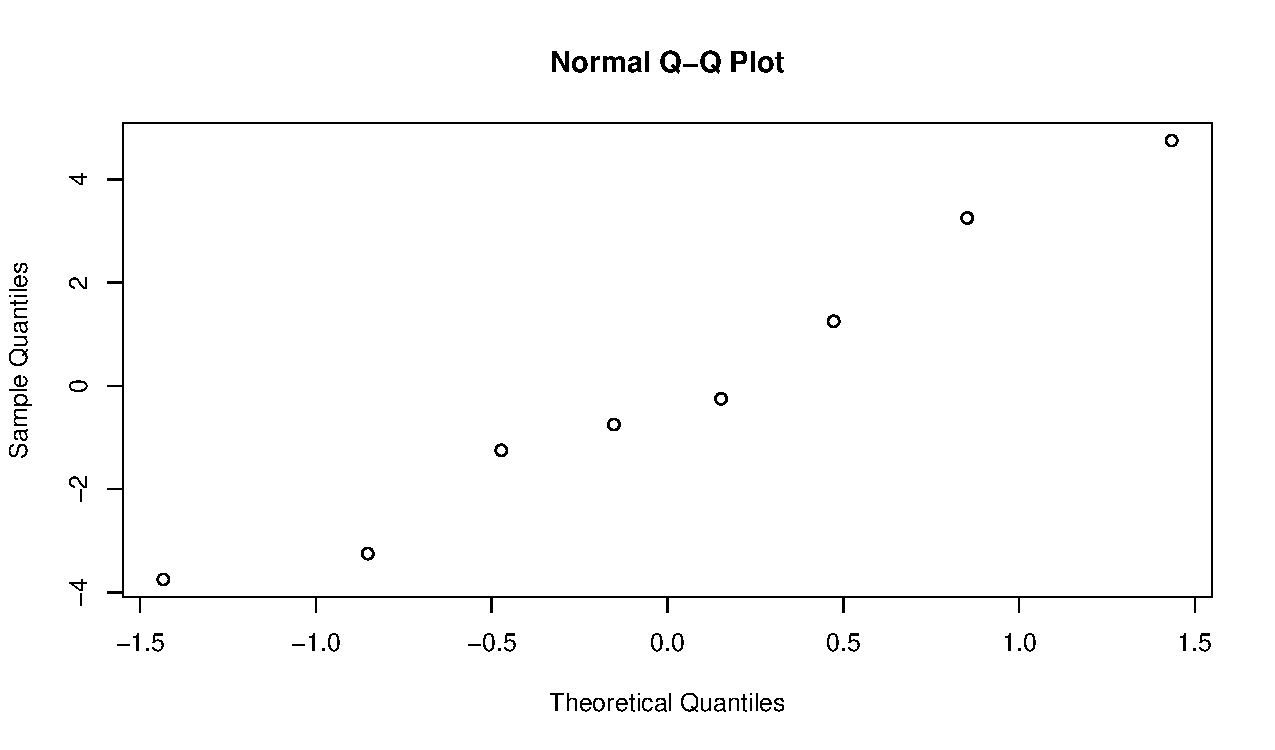
\includegraphics[width=\maxwidth]{figure/unnamed-chunk-16-1} 

}


\begin{kframe}\begin{alltt}
\hlkwd{plot}\hlstd{(model}\hlopt{$}\hlstd{residuals)}
\end{alltt}
\end{kframe}

{\centering 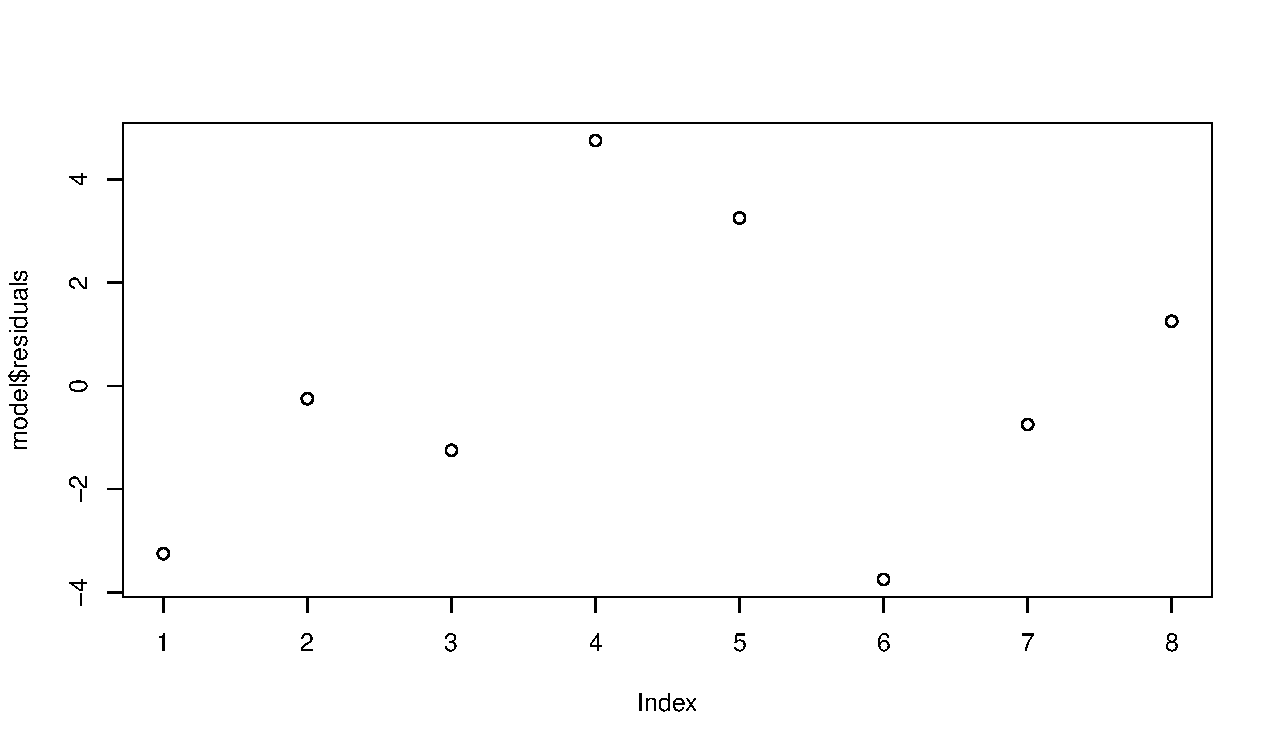
\includegraphics[width=\maxwidth]{figure/unnamed-chunk-16-2} 

}


\begin{kframe}\begin{alltt}
\hlkwd{plot}\hlstd{(model}\hlopt{$}\hlstd{fitted.values, model}\hlopt{$}\hlstd{residuals)}
\end{alltt}
\end{kframe}

{\centering 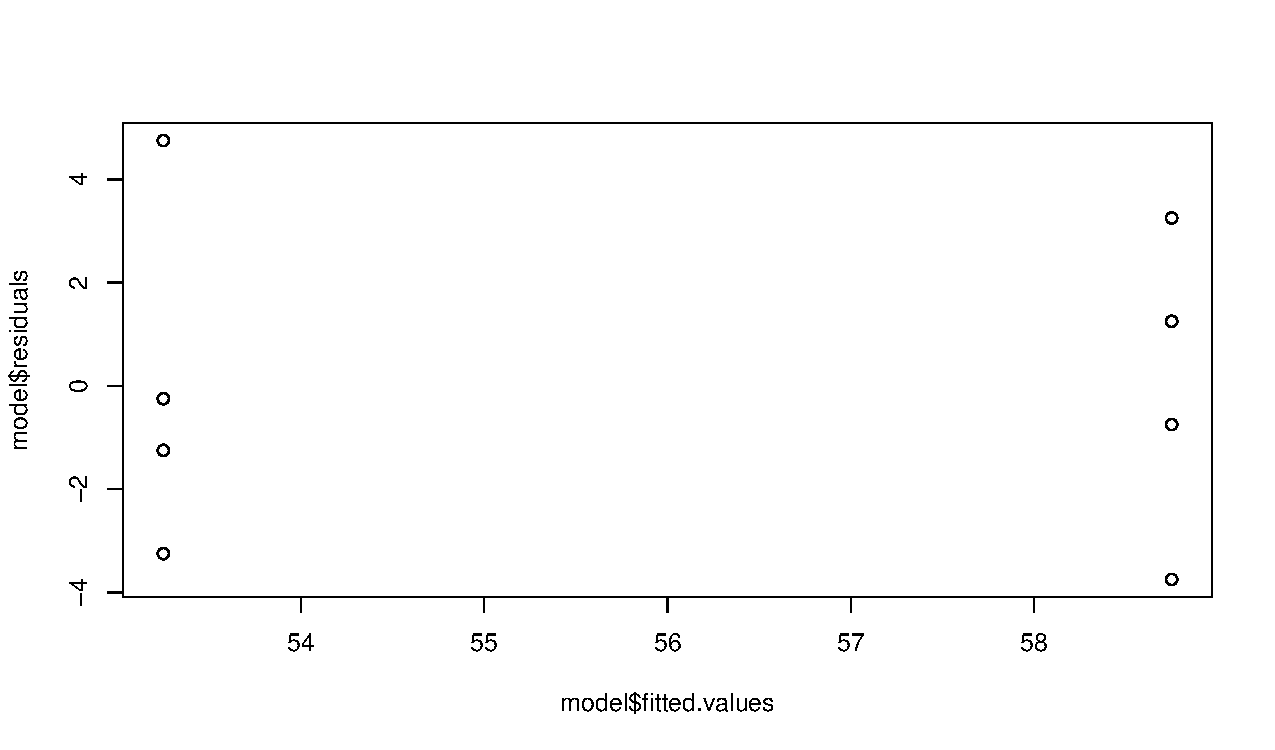
\includegraphics[width=\maxwidth]{figure/unnamed-chunk-16-3} 

}


\end{knitrout}

\section{Lecture 23.00: Model 5, Example 2}\label{section23}
Suppose professors are coordinating 4 sections
of the same course in a term. We want to look
at the average mark for each section on the midterm. The
treatment is the ``instructor.''
\begin{knitrout}
\definecolor{shadecolor}{rgb}{0.969, 0.969, 0.969}\color{fgcolor}\begin{kframe}
\begin{alltt}
\hlkwd{options}\hlstd{(}\hlkwc{contrasts} \hlstd{=} \hlkwd{c}\hlstd{(}\hlstr{"contr.sum"}\hlstd{,} \hlstr{"contr.poly"}\hlstd{))}
\hlstd{Marks1} \hlkwb{=} \hlkwd{c}\hlstd{(}\hlnum{55}\hlstd{,} \hlnum{92}\hlstd{,} \hlnum{48}\hlstd{,} \hlnum{57}\hlstd{,} \hlnum{66}\hlstd{,} \hlnum{72}\hlstd{)}
\hlstd{Marks2} \hlkwb{=} \hlkwd{c}\hlstd{(}\hlnum{62}\hlstd{,} \hlnum{95}\hlstd{,} \hlnum{84}\hlstd{,} \hlnum{83}\hlstd{,} \hlnum{66}\hlstd{,} \hlnum{75}\hlstd{)}
\hlstd{Marks3} \hlkwb{=} \hlkwd{c}\hlstd{(}\hlnum{89}\hlstd{,} \hlnum{92}\hlstd{,} \hlnum{94}\hlstd{,} \hlnum{99}\hlstd{,} \hlnum{87}\hlstd{,} \hlnum{67}\hlstd{)}
\hlstd{Marks4} \hlkwb{=} \hlkwd{c}\hlstd{(}\hlnum{25}\hlstd{,} \hlnum{35}\hlstd{,} \hlnum{71}\hlstd{,} \hlnum{42}\hlstd{,} \hlnum{44}\hlstd{,} \hlnum{30}\hlstd{)}
\hlstd{Y} \hlkwb{=} \hlkwd{c}\hlstd{(Marks1, Marks2, Marks3, Marks4)}
\hlstd{x} \hlkwb{=} \hlkwd{as.factor}\hlstd{(}\hlkwd{c}\hlstd{(}\hlkwd{rep}\hlstd{(}\hlnum{1}\hlstd{,} \hlnum{6}\hlstd{),} \hlkwd{rep}\hlstd{(}\hlnum{2}\hlstd{,} \hlnum{6}\hlstd{),} \hlkwd{rep}\hlstd{(}\hlnum{3}\hlstd{,} \hlnum{6}\hlstd{),} \hlkwd{rep}\hlstd{(}\hlnum{4}\hlstd{,} \hlnum{6}\hlstd{)))}
\hlstd{model} \hlkwb{=} \hlkwd{lm}\hlstd{(Y} \hlopt{~} \hlstd{x)}
\hlkwd{summary}\hlstd{(model)}
\end{alltt}
\begin{verbatim}
## 
## Call:
## lm(formula = Y ~ x)
## 
## Residuals:
##      Min       1Q   Median       3Q      Max 
## -21.0000 -10.2917   0.9167   6.1250  29.8333 
## 
## Coefficients:
##             Estimate Std. Error t value Pr(>|t|)    
## (Intercept)   67.917      2.861  23.741    4e-16 ***
## x1            -2.917      4.955  -0.589 0.562699    
## x2             9.583      4.955   1.934 0.067381 .  
## x3            20.083      4.955   4.053 0.000621 ***
## ---
## Signif. codes:  0 '***' 0.001 '**' 0.01 '*' 0.05 '.' 0.1 ' ' 1
## 
## Residual standard error: 14.01 on 20 degrees of freedom
## Multiple R-squared:  0.6506,	Adjusted R-squared:  0.5982 
## F-statistic: 12.41 on 3 and 20 DF,  p-value: 8.281e-05
\end{verbatim}
\end{kframe}
\end{knitrout}
Note that
\begin{itemize}
    \item $ \hat{\tau}_4=-(\hat{\tau}_1+\hat{\tau}_2+\hat{\tau}_3)=-26.749 $.
    \item $ \text{Degrees of freedom}=n-q+c=(24)-(4+1)+1=20 $.
\end{itemize}
\subsection*{Is there a difference between the treatment effect of group 1 and 2? Use a 95\% CI.}
$ \tilde{\theta}=\tilde{\tau}_1+\tilde{\tau}_2 $ and by Gauss this is normal.
\[ \E{\tilde{\theta}}=\E{\tilde{\tau}_1-\tilde{\tau}_2}=\tau_1+\tau_2 \]
\[ \Var{\tilde{\theta}}=\Var{\tilde{\tau}_1-\tilde{\tau}_2}
    =\Var{\bar{Y}_{1+}-\bar{Y}_{2+}}
    =\Var{\bar{Y}_{1+}}+\Var{\bar{Y}_{2+}}
    =\frac{\sigma^2}{6} +\frac{\sigma^2}{6}
    =\frac{\sigma^2}{3} \]
The 95\% confidence interval for $ \theta $ is
\[ \hat{\tau}_1-\hat{\tau}_2 \pm c\, \frac{\hat{\sigma}}{\sqrt{3}}=
    -2.917-9.583\pm \frac{2.09(14.01)}{\sqrt{3}}=(-29.37,4.37) \quad(c \sim t(20))  \]
In R, we could do
\begin{knitrout}
\definecolor{shadecolor}{rgb}{0.969, 0.969, 0.969}\color{fgcolor}\begin{kframe}
\begin{alltt}
\hlstd{tau.1} \hlkwb{<-} \hlkwd{summary}\hlstd{(model)}\hlopt{$}\hlstd{coefficients[}\hlnum{2}\hlstd{]}
\hlstd{tau.2} \hlkwb{<-} \hlkwd{summary}\hlstd{(model)}\hlopt{$}\hlstd{coefficients[}\hlnum{3}\hlstd{]}
\hlstd{tau.3} \hlkwb{<-} \hlkwd{summary}\hlstd{(model)}\hlopt{$}\hlstd{coefficients[}\hlnum{4}\hlstd{]}
\hlstd{tau.4} \hlkwb{<-} \hlopt{-}\hlnum{1} \hlopt{*} \hlstd{(tau.1} \hlopt{+} \hlstd{tau.2} \hlopt{+} \hlstd{tau.3)}
\hlstd{tau.1} \hlopt{-} \hlstd{tau.2} \hlopt{+} \hlkwd{c}\hlstd{(}\hlopt{-}\hlnum{1}\hlstd{,} \hlnum{1}\hlstd{)} \hlopt{*} \hlkwd{qt}\hlstd{(}\hlnum{0.975}\hlstd{,} \hlnum{20}\hlstd{)} \hlopt{*} \hlkwd{summary}\hlstd{(model)}\hlopt{$}\hlstd{sigma}\hlopt{/}\hlkwd{sqrt}\hlstd{(}\hlnum{3}\hlstd{)}
\end{alltt}
\begin{verbatim}
## [1] -29.378554   4.378554
\end{verbatim}
\end{kframe}
\end{knitrout}
To get at 95\% confidence interval $ \theta $: $ (-29.38,4.38) $.
Since $ 0\in (-29.38,4.38) $,
there is not a difference between the treatment effect of group 1 and 2.

\subsection*{Groups 2 and 3 were taught by the same instructor. Groups 1 and 4 are taught by another
    instructor. Is there a difference between the average treatment effect of instructor 1 to instructor 2? Use an
    HT.}
\[ \tilde{\theta}=\frac{\tilde{\tau}_1+\tilde{\tau}_4}{2}-\biggl(\frac{\tilde{\tau}_2+\tilde{\tau}_3}{2} \biggr)  \]
\[ \E{\tilde{\theta}}=\frac{\tau_1+\tau_4}{2}-\biggl(\frac{\tau_2+\tau_3}{2} \biggr) \]
\begin{align*}
    \Var{\tilde{\theta}}
     & =\Var*{\frac{\tilde{\tau}_1+\tilde{\tau}_4}{2}-\biggl(\frac{\tilde{\tau}_2+\tilde{\tau}_3}{2} \biggr) } \\
     & =\Var*{\frac{\bar{Y}_{1+}+\bar{Y}_{4+}}{2}-\biggl(\frac{\bar{Y}_{2+}+\bar{Y}_{3+}}{2} \biggr)}          \\
     & =\frac{1}{4} \Var{Y_{1+}}+\cdots+\frac{1}{4} \Var{Y_{4+}}                                               \\
     & =\frac{\sigma^2}{4(6)}+\cdots+\frac{\sigma^2}{4(6)}                                                     \\
     & =\frac{\sigma^2}{6}
\end{align*}
$ H_0 $: $ \theta=0 $ versus $ H_a $: $ \theta\ne 0 $.
\[ d=\frac{\hat{\theta}-0}{\hat{\sigma}/\sqrt{6}}=-5.19\quad(D \sim t(20))  \]
\[ p=2\Prob{D>\abs{-5.19}}=(0,0.001) \]
We have tons of evidence to reject $ H_0 $ in favour
of the instructors having a different effect. In R, we could do
\begin{knitrout}
\definecolor{shadecolor}{rgb}{0.969, 0.969, 0.969}\color{fgcolor}\begin{kframe}
\begin{alltt}
\hlstd{theta} \hlkwb{<-} \hlstd{((tau.1} \hlopt{+} \hlstd{tau.4)}\hlopt{/}\hlnum{2}\hlstd{)} \hlopt{-} \hlstd{((tau.2} \hlopt{+} \hlstd{tau.3)}\hlopt{/}\hlnum{2}\hlstd{)}
\hlstd{d} \hlkwb{<-} \hlstd{(theta} \hlopt{-} \hlnum{0}\hlstd{)}\hlopt{/}\hlstd{(}\hlkwd{summary}\hlstd{(model)}\hlopt{$}\hlstd{sigma}\hlopt{/}\hlkwd{sqrt}\hlstd{(}\hlnum{6}\hlstd{))}
\hlstd{d}
\end{alltt}
\begin{verbatim}
## [1] -5.185077
\end{verbatim}
\begin{alltt}
\hlnum{2} \hlopt{*} \hlstd{(}\hlnum{1} \hlopt{-} \hlkwd{pt}\hlstd{(}\hlkwd{abs}\hlstd{(d),} \hlnum{20}\hlstd{))}
\end{alltt}
\begin{verbatim}
## [1] 4.498007e-05
\end{verbatim}
\end{kframe}
\end{knitrout}
    To obtain a $ p $-value of $ 4.498007\times 10^{-5} $.
\begin{Example}{}{}
    An example of a \emph{contrast} is
    \[ \theta=\frac{\tau_1+\tau_4}{2} -\frac{(\tau_2+\tau_3)}{2}  \]
\end{Example}
\begin{Definition}{Contrast}{}
    A \textbf{contrast} has the form
    \[ a_1\tau_1+a_2\tau_2+\cdots+a_n\tau_n \]
    where $ \sum_{i=1}^{n} a_i=0 $.
\end{Definition}
\makeheading{2020-03-06}
\section{Burst Error Correcting}
``Cyclic codes are good for (cyclic) burst error correcting.''

Suppose we have a $ C:(n,k,d) $ code, with $ e=\lfloor \frac{d-1}{2} \rfloor=5 $.
In practice, errors typically happen in bursts (not spread out).
We expect typically one burst per codeword, or bursts to carry through
two codewords.

\begin{defbox}
    \begin{definition}
        Let $ \bm{e}\in V_n(F) $. The \textbf{cyclic burst length of $\bm{e}$}
        is the length of the smallest cyclic block that contain all the non-zero
        entries of $ \bm{e} $.
    \end{definition}
\end{defbox}

\begin{exbox}
    \begin{example}
        $ \bm{e}=\bm{011}00000\bm{1} $ has cyclic burst length $ 4 $.
    \end{example}
\end{exbox}

\begin{defbox}
    \begin{definition}
        We say $ \bm{e} $ is a \textbf{cyclic burst error of length $ \bm{t} $} if its cyclic
        burst length is $ t $.
    \end{definition}
\end{defbox}

\begin{defbox}
    \begin{definition}
        A linear code $ C $ is a \textbf{$ \bm{t} $-cyclic burst error correcting code}
        if every cyclic burst error of length at most $ t $ lies in a unique coset
        of $ C $. The largest such $ t $ is called the \textbf{cyclic burst error capability
            of $ \bm{C} $}.
    \end{definition}
\end{defbox}

\begin{exbox}
    \begin{example}
        $ g(x)=1+x+x^2+x^3+x^6 $ generates a $ (15,9) $-binary cyclic code $ C $
        that is a $ 3 $-cyclic burst error correcting code.
    \end{example}
\end{exbox}

$ d(C)\leqslant 5 $, so $ e\leqslant 2 $. We verify this by checking that
each cyclic burst of length $ \leqslant 3 $ has a unique syndrome.

\begin{table}[H]
    \centering
    \begin{tabularx}{\linewidth}{@{}YYY@{}}
        Cyclic burst errors & Syndromes  & Notes                                   \\
        \midrule
        \midrule
        0                   & 000000                                               \\
        \midrule
        $ x^0 $             & 100000                                               \\
        $ x^1 $             & 010000                                               \\
        $ x^2 $             & 001000                                               \\
        $ x^3 $             & 000100                                               \\
        $ x^4 $             & 000010                                               \\
        $ x^5 $             & 000001                                               \\
        $ x^6 $             & 111100     & $ x^6+g(x)\iff (0000001)+(1111001) $    \\
        $ x^7 $             & 011110                                               \\
        $ x^8 $             & 001111                                               \\
        $ x^9 $             & 111011     & $ x^9+g(x)\iff (0001111)+(1111001) $    \\
        $ x^{10} $          & 100001     & $ x^{10}+g(x)\iff (0111011)+(1111001) $ \\
        $ x^{11} $          & 101100     & $ x^{11}+g(x)\iff (0100001)+(1111001) $ \\
        $ x^{12} $          & 010110                                               \\
        $ x^{13} $          & 001011                                               \\
        $ x^{14} $          & 111001     & $ x^{14}+g(x)\iff (0001011)+(1111001) $ \\
        \midrule
        $ 1+x $             & 110000                                               \\
        $ x(1+x) $          & 011000                                               \\
        $ \vdots $          & $ \vdots $                                           \\
        $ x^{14}(1+x) $     & 011001                                               \\
        \midrule
        $ 1+x+x^2 $         & 111000                                               \\
        $ x(1+x+x^2) $      & 011100                                               \\
        $ \vdots $          & $ \vdots $                                           \\
        $ x^{14}(1+x+x^2) $ & 001001                                               \\
        \midrule
        $ 1+x^2 $           & 101000                                               \\
        $ x(1+x^2) $        & 010100                                               \\
        $ \vdots $          & $ \vdots $                                           \\
        $ x^{14}(1+x^2) $   & 101001                                               \\
    \end{tabularx}
\end{table}
The number of cyclic bursts of length $ \leqslant 3 $ is $ 61 $.
The number of syndromes is $ 64 $.

\begin{exbox}
    \begin{example}
        $ g(x)=1+x^4+x^6+x^7+x^8 $ generates a $ (15,7) $-binary cyclic
        code that is $ 4 $-cyclic burst error correcting.
        Distance $ \leqslant 5 $ so $ e\leqslant 2 $.
    \end{example}
\end{exbox}

\textbf{Question}: How to construct codes with high cyclic burst error
correcting capability?
\begin{enumerate}[label=(\arabic*)]
    \item Use a computer search
    \item RS Codes
    \item Interleaving
\end{enumerate}

\begin{thmbox}
    \begin{theorem}
        Let $ C $ be an $ (n,k,d) $-code over $ GF(q) $. Let $ t $ be its
        cyclic burst error correcting capability.
        \[ \left\lfloor \frac{d-1}{2} \right\rfloor \leqslant t \leqslant n-k \]
    \end{theorem}
\end{thmbox}

\begin{proof}
    Every cyclic burst of length $ \leqslant t $ has weight $ \leqslant t $.
    Since every vector of weight $ \leqslant \lfloor \frac{d-1}{2} \rfloor $
    has a unique syndrome, we have $ \lfloor \frac{d-1}{2} \rfloor \leqslant t $.

    The number of cyclic burst errors where all the non-zero entries lie in the first
    $ t $ coordinate positions is $ q^t $. Each of them has a unique coset
    and the total number of cosets is $ q^{n-k} $. Thus,
    \[ q^t\leqslant q^{n-k}\implies t\leqslant n-k \]
\end{proof}

Exercise: Prove that $ t\leqslant \frac{n-k}{2} $.

\section{Decoding Cyclic Burst Errors}
Let $ C $ be a $ t $-cyclic burst error correcting code generated
by $ g(x) $ which is a degree-$ k $ monic divisor of $ x^n-1 $ over $ GF(q) $.

Recall: A PCM for $ C $ is:
\[ H= \Bigl[\; I_{n-k}\mid -R^\top \;\Bigr] \]

whose columns are $ x^0 \mod g(x),\ldots ,x^{n-1} \mod g(x) $.

The syndrome of $ r(x) $ is $ s(x)\equiv r(x)\mod g(x) $.

\textbf{Idea:} Suppose $ \bm{e} $ is a cyclic burst of length $ \leqslant t $.

Compute $ \bm{s}=H\bm{r}^\top\equiv r(x)\mod g(x) $.

Suppose $ \bm{e}= $ \fbox{x o $ \cdots $ o x x x} . We multiply $ x^3 $ by $ \bm{e} $,
so we get \fbox{x x x x o $ \cdots $ o}.

$ \bm{s}=H\bm{r}^\top=H\bm{e}^\top $.

$ \bm{s}_1=H(x\bm{r})^\top = H(x\bm{e})^\top $

$ \bm{s}_2=H(x^2\bm{r})^\top = H(x^2\bm{e})^\top $

$ \bm{s}_3=H(x^3\bm{r})^\top = H(x^3\bm{e})^\top $

\section{Lecture 25.00: F Test}
\begin{figure}[!htbp]
    \centering
    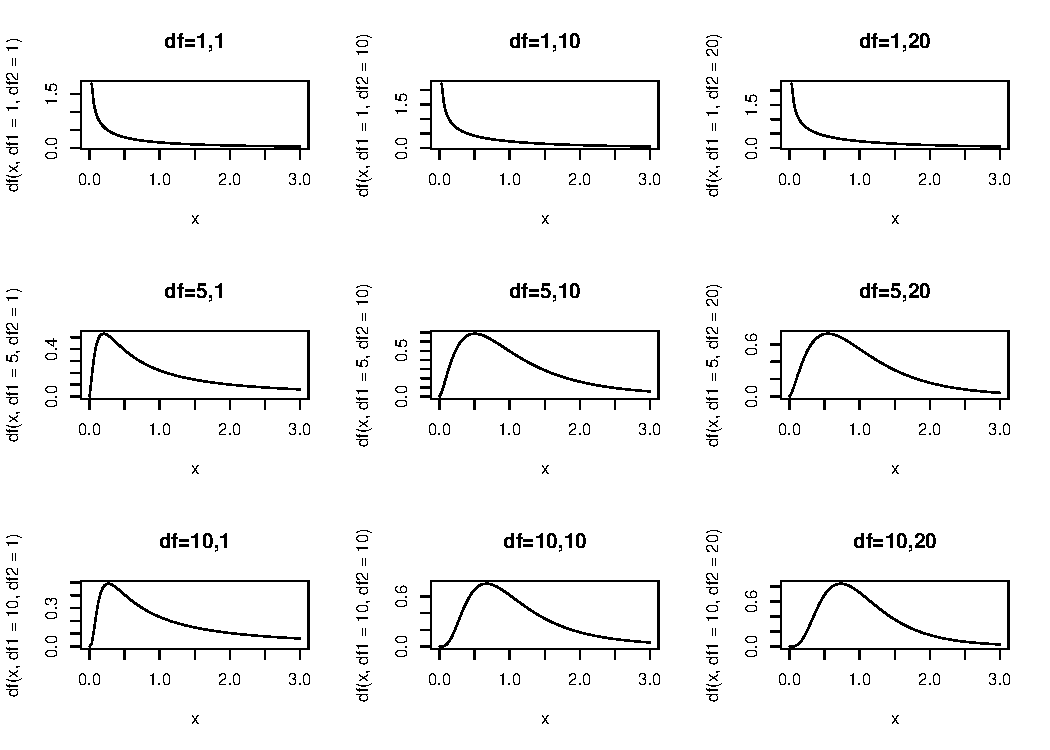
\includegraphics[width=0.7\textwidth]{fdistn.pdf}
    \caption{$ F $ distribution}
\end{figure}
\begin{Theorem}{}{}
    Let $ X \sim \chi^2(m) $ and $ Y \sim \chi^2(n) $, then
    \[ \frac{X/m}{Y/n} \sim F(m,n) \]
\end{Theorem}
\begin{Theorem}{}{}
    Let $ X \sim F(m,n) $ and $ Y \sim 1/X $, then
    \[ Y \sim F(n,m) \]
\end{Theorem}
\begin{Example}{}{}
    $ \alpha=\Prob{F(20,4)>4}=(0.05,0.1) $ since
    \begin{center}
        \begin{NiceTabular}{c|ccc}
            $\alpha$       & 0.1  & 0.05 & 0.01 \\
            \midrule
            critical value & 3.84 & 5.80 & 14.0
        \end{NiceTabular}
    \end{center}
    In R, we can directly calculate $ \alpha $ with \code{1-pf(4,20,4)=0.094}.
\end{Example}
\[ \tilde{F}=\frac{\widetilde{\MS{Trt}}}{\widetilde{\MS{Res}}}  \]
Now, $ \widetilde{\MS{Res}}=\tilde{\sigma}^2 $. We know
\begin{equation}\label{eq:1}
    \frac{\tilde{\sigma}^2\text{df}_\text{Res}}{\sigma^2} \sim \chi^2(\text{df}_{\text{Res}})
\end{equation}
Similarly,
\begin{equation}\label{eq:2}
    \frac{\widetilde{\MS{Trt}}\text{df}_\text{Trt}}{\sigma^2} \sim \chi^2(\text{df}_\text{Trt})
\end{equation}
Divide~\ref{eq:2} by~\ref{eq:1} to get
\[ \frac{\widetilde{\MS{Trt}}}{\widetilde{\MS{Res}}} \sim F(n,d) \]
where $ n=\text{df}_\text{Trt} $ and $ d=\text{df}_\text{Res} $.

\subsection*{When is $ F $ large?}
\[ \E{\tilde{F}}=
    \E*{\frac{\widetilde{\MS{Trt}}}{\widetilde{\MS{Res}}}}{\color{red}\approx}
    \frac{\E{\widetilde{\MS{Trt}}}}{\E{\widetilde{\MS{Res}}}}
    =\frac{\sigma^2+r \dfrac{\sum_{i=1}^t \tau_i^2}{t-1} }{\sigma^2}  \]
\[ \E{\tilde{F}}=1+\frac{r}{\sigma^2} \frac{\sum_{i=1}^t \tau_i^2 }{t-1}  \]
If $ \tau_1=\tau_2=\cdots=\tau_t=0 $, then $ \E{\tilde{F}}=1 $.
However, if even one $ \tau $ is not zero, then $ \E{\tilde{F}}>1 $.

\subsection*{$F$ Test}
\begin{enumerate}[(1)]
    \item $ H_0 $: $ \tau_1=\tau_2=\cdots=\tau_t=0 $ versus $ H_a $: at least one $\tau$ is not zero.
    \item $ \displaystyle d=\frac{\MS{Trt}}{\MS{Res}}  $ where $ D \sim F(\text{df}_\text{Trt},\text{df}_\text{Res}) $
    \item $ p\text{-value}=\Prob{D>d} $
    \item Conclusion.
\end{enumerate}


\section{Lecture 26.00: F Test, Example}

See~\Cref{section23} for the data.

\begin{knitrout}
\definecolor{shadecolor}{rgb}{0.969, 0.969, 0.969}\color{fgcolor}\begin{kframe}
\begin{alltt}
\hlkwd{anova}\hlstd{(model)}
\end{alltt}
\begin{verbatim}
## Analysis of Variance Table
## 
## Response: Y
##           Df Sum Sq Mean Sq F value    Pr(>F)    
## x          3 7315.5 2438.50  12.415 8.281e-05 ***
## Residuals 20 3928.3  196.42                      
## ---
## Signif. codes:  0 '***' 0.001 '**' 0.01 '*' 0.05 '.' 0.1 ' ' 1
\end{verbatim}
\end{kframe}
\end{knitrout}
\begin{itemize}
    \item $ H_0 $: $ \tau_1=\tau_2=\tau_3=\tau_4=0 $
    \item $ H_a $: At least one $ \tau $ is not zero
\end{itemize}
\[ d=\frac{\MS{Trt}}{\MS{Res}} =\frac{\SS{Trt}/\text{df}_\text{Trt}}{\SS{Res}/\text{df}_\text{Res}}
    =\frac{7315.5/3}{3928.3/20}=12.415   \]
Note that $ D \sim F(3,20) $, so
\[ p=\Prob{D>12.415}=8.21 \times 10^{-5} \]
We have tons of evidence against $ H_0 $, so one of our treatment effects is not zero.


\chapter{Assignment 4}
\section{Lecture 27.00: Model 6}
\begin{Definition}{Unbalanced CRD, Model 6}{}
    The \textbf{unbalanced completely randomized design} is
    \[ Y_{ij}=\mu+\tau_i+R_{ij}\quad(R_{ij}\sim \N{0,\sigma^2}) \]
    for $ i=1,2,\ldots,t $ (no.\ of treatments),
    $ j=1,2,\ldots,r_i $ (no.\ of replicates/treatment).
    In this course, this is \textbf{Model 6}.

    \underline{Constraint}: $ \sum_{i=1}^{t} r_i \tau_i=0 $.
\end{Definition}
\begin{Example}{LS for Model 6}{}
    The LS for Model 6 is
    \[ W=\sum r_{ij}^2 +\lambda\biggl(\sum_{i=1}^{t} r_i\tau_i\biggr)  \]
    and results in
    \[ \hat{\mu}=\bar{y}_{++} \]
    \[ \hat{\tau}_i=\bar{y}_{i+}-\bar{y}_{++} \]
    \[ \hat{\sigma}^2=\frac{W}{(r_1+r_2+\cdots+r_t)-(t+1)+1}  \]
\end{Example}
\subsection{Unbalanced CRD Example}
Refer to~\Cref{section21}, we remove the last element of group 2.
\begin{knitrout}
\definecolor{shadecolor}{rgb}{0.969, 0.969, 0.969}\color{fgcolor}\begin{kframe}
\begin{alltt}
\hlstd{grp1} \hlkwb{=} \hlkwd{c}\hlstd{(}\hlnum{50}\hlstd{,} \hlnum{53}\hlstd{,} \hlnum{52}\hlstd{,} \hlnum{58}\hlstd{)}
\hlstd{grp2} \hlkwb{=} \hlkwd{c}\hlstd{(}\hlnum{62}\hlstd{,} \hlnum{55}\hlstd{,} \hlnum{58}\hlstd{)}
\hlstd{Y} \hlkwb{=} \hlkwd{c}\hlstd{(grp1, grp2)}
\hlstd{x} \hlkwb{=} \hlkwd{as.factor}\hlstd{(}\hlkwd{c}\hlstd{(}\hlkwd{rep}\hlstd{(}\hlnum{1}\hlstd{,} \hlnum{4}\hlstd{),} \hlkwd{rep}\hlstd{(}\hlnum{2}\hlstd{,} \hlnum{3}\hlstd{)))}
\hlcom{# Group Averages}
\hlstd{grp_av} \hlkwb{=} \hlkwd{tapply}\hlstd{(Y, x, mean,} \hlkwc{na.rm} \hlstd{= T)}
\hlstd{mu} \hlkwb{=} \hlkwd{mean}\hlstd{(Y)}
\hlcom{# Treatment Effects}
\hlstd{tau1} \hlkwb{=} \hlstd{(grp_av} \hlopt{-} \hlkwd{mean}\hlstd{(Y))[}\hlnum{1}\hlstd{]}
\hlstd{tau2} \hlkwb{=} \hlstd{(grp_av} \hlopt{-} \hlkwd{mean}\hlstd{(Y))[}\hlnum{2}\hlstd{]}
\hlcom{# Estimated Sigma}
\hlstd{sigma} \hlkwb{=} \hlkwd{summary}\hlstd{(}\hlkwd{lm}\hlstd{(Y} \hlopt{~} \hlstd{x))}\hlopt{$}\hlstd{sigma}
\hlcom{# Values}
\hlstd{sigma}
\end{alltt}
\begin{verbatim}
## [1] 3.447221
\end{verbatim}
\begin{alltt}
\hlstd{tau1}
\end{alltt}
\begin{verbatim}
##         1 
## -2.178571
\end{verbatim}
\begin{alltt}
\hlstd{tau2}
\end{alltt}
\begin{verbatim}
##        2 
## 2.904762
\end{verbatim}
\begin{alltt}
\hlstd{mu}
\end{alltt}
\begin{verbatim}
## [1] 55.42857
\end{verbatim}
\end{kframe}
\end{knitrout}
    We obtain
    \begin{itemize}
        \item $ \hat{\sigma}=3.447221 $
        \item $ \hat{\tau}_1=-2.178571 $
        \item $ \hat{\tau}_2=2.904762 $
        \item $ \hat{\mu}=55.42857 $
        \item Obviously, $ 4(\hat{\tau}_1)+3(\hat{\tau}_2)=0 $
    \end{itemize}
    \subsubsection*{What is the treatment effect for being inebriated?}
$ \hat{\tau}_1=-2.18 $
    \subsubsection*{Is there a difference between the treatment effect of group 1 and 2? Use a 95\% CI.}
$ \theta=\tau_1-\tau_2\implies \tilde{\theta}=\tilde{\tau}_1-\tilde{\tau}_2 $.
\[ \E{\tilde{\theta}}=\tau_1-\tau_2 \]
\[ \Var{\tilde{\theta}}=\Var{\bar{Y}_{1+}-\bar{Y}_{2+}}=\frac{\sigma^2}{4} +\frac{\sigma^2}{3}=\frac{7\sigma^2}{12}  \]
Confidence interval:
\[ \hat{\tau}_1-\hat{\tau}_2\pm c\sqrt{\frac{7\hat{\sigma}^2}{12}}=(-11.85,1.68) \]
In R,
\begin{knitrout}
\definecolor{shadecolor}{rgb}{0.969, 0.969, 0.969}\color{fgcolor}\begin{kframe}
\begin{alltt}
\hlstd{tau1} \hlopt{-} \hlstd{tau2} \hlopt{+} \hlkwd{c}\hlstd{(}\hlopt{-}\hlnum{1}\hlstd{,} \hlnum{1}\hlstd{)} \hlopt{*} \hlkwd{qt}\hlstd{(}\hlnum{0.975}\hlstd{,} \hlnum{5}\hlstd{)} \hlopt{*} \hlkwd{sqrt}\hlstd{((}\hlnum{7} \hlopt{*} \hlstd{sigma}\hlopt{^}\hlnum{2}\hlstd{)}\hlopt{/}\hlnum{12}\hlstd{)}
\end{alltt}
\begin{verbatim}
## [1] -11.851312   1.684645
\end{verbatim}
\end{kframe}
\end{knitrout}
\subsubsection*{Is there a difference between the treatment effect of group 1 and 2? Use a HT.}
\begin{knitrout}
\definecolor{shadecolor}{rgb}{0.969, 0.969, 0.969}\color{fgcolor}\begin{kframe}
\begin{alltt}
\hlkwd{anova}\hlstd{(}\hlkwd{lm}\hlstd{(Y} \hlopt{~} \hlstd{x))}
\end{alltt}
\begin{verbatim}
## Analysis of Variance Table
## 
## Response: Y
##           Df Sum Sq Mean Sq F value Pr(>F)
## x          1 44.298  44.298  3.7277 0.1114
## Residuals  5 59.417  11.883
\end{verbatim}
\end{kframe}
\end{knitrout}
No evidence against $ H_0 $: $ \tau_1=\cdots=\tau_t=0 $, so this model is not great.
\section{Lecture 28.00: Model 7}
\begin{Definition}{Randomized block design, Model 7}{}
    The \textbf{randomized block design} (RBD) is defined as
    \[ Y_{ij}=\mu+\tau_i+\beta_j+R_{ij}\quad(R_{ij} \sim \N{0,\sigma^2}) \]
    where $ \beta_j $ is the $ j^{\text{th}} $ block (BIK) effect. Note that
    \begin{itemize}
        \item $ i=1,2,\ldots,t $
        \item $ j=1,2,\ldots,r $
        \item $ \sum_{i=1}^t \tau_i=0  $
        \item $\sum_{j=1}^{r} \beta_j=0$
    \end{itemize}
\end{Definition}
\begin{Example}{LS for Model 7}{}
    The LS for Model 7 is
    \[ W=\sum_{ij}r_{ij}+\lambda_1\biggl(\sum_{i=1}^{t} \tau_i\biggr)+
        \lambda_2 \biggl(\sum_{j=1}^{r} \beta_j\biggr)  \]
    Solving
    \[ \hat{\mu}=\bar{y}_{++} \]
    \[ \hat{\tau}_i=\bar{y}_{i+}-\bar{y}_{++} \]
    \[ \hat{\beta}_j=\bar{y}_{+j}-\bar{y}_{++} \]
    \[ \hat{\sigma}^2=\frac{W}{(rt)-(t+r+1)+2} \]
\end{Example}


\section{Lecture 29.00: Model 7, Example}
We grow willow trees from cuttings. We grow these cuttings from 6 willow trees in
two soils: high and low acidity. We assign two cuttings from each tree to the two levels of
acidity. After 1 year the height, we measure the cuttings in centimetres.
\subsection*{Is the growth in high and low acidity equal? Use an appropriate hypothesis test.}
\begin{knitrout}
\definecolor{shadecolor}{rgb}{0.969, 0.969, 0.969}\color{fgcolor}\begin{kframe}
\begin{alltt}
\hlcom{# Step 1 – Change the directory In R, select FILE, CHANGE}
\hlcom{# DIR select the folder your data is located in.}
\hlcom{# Step 2 – use read.table}
\hlstd{Data} \hlkwb{=} \hlkwd{read.table}\hlstd{(}\hlstr{"blocked.csv"}\hlstd{,} \hlkwc{sep} \hlstd{=} \hlstr{","}\hlstd{,} \hlkwc{header} \hlstd{= T)}
\hlcom{# Step 3 – Have a look at the data:}
\hlstd{Data}
\end{alltt}
\begin{verbatim}
##    Block Treatment Value
## 1      1      High    16
## 2      2      High    19
## 3      3      High    32
## 4      4      High    12
## 5      5      High     7
## 6      6      High    14
## 7      1       Low    17
## 8      2       Low    21
## 9      3       Low    33
## 10     4       Low    11
## 11     5       Low     8
## 12     6       Low    12
\end{verbatim}
\begin{alltt}
\hlcom{# To build a model we type:}
\hlkwd{options}\hlstd{(}\hlkwc{contrasts} \hlstd{=} \hlkwd{c}\hlstd{(}\hlstr{"contr.sum"}\hlstd{,} \hlstr{"contr.poly"}\hlstd{))}
\hlkwd{attach}\hlstd{(Data)}
\hlstd{Treatment} \hlkwb{=} \hlkwd{as.factor}\hlstd{(Treatment)}
\hlstd{Block} \hlkwb{=} \hlkwd{as.factor}\hlstd{(Block)}
\hlstd{Model} \hlkwb{=} \hlkwd{lm}\hlstd{(Value} \hlopt{~} \hlstd{Treatment} \hlopt{+} \hlstd{Block)}
\hlcom{# To look at the output, we type:}
\hlkwd{summary}\hlstd{(Model)}
\end{alltt}
\begin{verbatim}
## 
## Call:
## lm(formula = Value ~ Treatment + Block)
## 
## Residuals:
##       1       2       3       4       5       6       7       8       9      10 
## -0.3333 -0.8333 -0.3333  0.6667 -0.3333  1.1667  0.3333  0.8333  0.3333 -0.6667 
##      11      12 
##  0.3333 -1.1667 
## 
## Coefficients:
##             Estimate Std. Error t value Pr(>|t|)    
## (Intercept)  16.8333     0.3073  54.775 3.84e-08 ***
## Treatment1   -0.1667     0.3073  -0.542 0.610881    
## Block1       -0.3333     0.6872  -0.485 0.648131    
## Block2        3.1667     0.6872   4.608 0.005797 ** 
## Block3       15.6667     0.6872  22.798 3.02e-06 ***
## Block4       -5.3333     0.6872  -7.761 0.000568 ***
## Block5       -9.3333     0.6872 -13.582 3.88e-05 ***
## ---
## Signif. codes:  0 '***' 0.001 '**' 0.01 '*' 0.05 '.' 0.1 ' ' 1
## 
## Residual standard error: 1.065 on 5 degrees of freedom
## Multiple R-squared:  0.9927,	Adjusted R-squared:  0.984 
## F-statistic: 113.5 on 6 and 5 DF,  p-value: 3.532e-05
\end{verbatim}
\begin{alltt}
\hlkwd{anova}\hlstd{(Model)}
\end{alltt}
\begin{verbatim}
## Analysis of Variance Table
## 
## Response: Value
##           Df Sum Sq Mean Sq  F value    Pr(>F)    
## Treatment  1   0.33   0.333   0.2941    0.6109    
## Block      5 771.67 154.333 136.1765 2.446e-05 ***
## Residuals  5   5.67   1.133                       
## ---
## Signif. codes:  0 '***' 0.001 '**' 0.01 '*' 0.05 '.' 0.1 ' ' 1
\end{verbatim}
\end{kframe}
\end{knitrout}

\begin{itemize}
    \item $ \hat{\sigma}=1.065 $ on $ n-q+c $ degrees of freedom.
          In this case, we have 6 blocks, 2 treatments, so 12 total values.
          One $ \mu $ and two constraints. So $ 12-6-2-1+2=5 $ degrees of freedom.
    \item $ \tilde{\theta}=\tilde{\tau}_1-\tilde{\tau}_2 $.
    \item $ \E{\tilde{\theta}}=\tau_1-\tau_2 $.
    \item $ \displaystyle \Var{\tilde{\theta}}=\Var{\bar{Y}_{1+}}-\Var{\bar{Y}_{2+}}
              =\frac{\sigma^2}{6} +\frac{\sigma^2}{6}
              =\frac{\sigma^2}{3} $.
\end{itemize}
The confidence interval for the difference in treatments is:
\[ \hat{\tau}_1-\hat{\tau}_2\pm c \sqrt{\frac{\hat{\sigma}^2}{3}}
    =(-0.1667-0.1667)\pm 2.57 \frac{1.065}{\sqrt{3}} =(-1.91, 1.25) \]
\subsection*{Suppose we ran a CRD instead.}
\begin{knitrout}
\definecolor{shadecolor}{rgb}{0.969, 0.969, 0.969}\color{fgcolor}\begin{kframe}
\begin{alltt}
\hlstd{Model} \hlkwb{=} \hlkwd{lm}\hlstd{(Value} \hlopt{~} \hlstd{Treatment)}
\hlkwd{summary}\hlstd{(Model)}
\end{alltt}
\begin{verbatim}
## 
## Call:
## lm(formula = Value ~ Treatment)
## 
## Residuals:
##    Min     1Q Median     3Q    Max 
## -9.667 -5.250 -1.667  2.750 16.000 
## 
## Coefficients:
##             Estimate Std. Error t value Pr(>|t|)    
## (Intercept)  16.8333     2.5451   6.614 5.97e-05 ***
## Treatment1   -0.1667     2.5451  -0.065    0.949    
## ---
## Signif. codes:  0 '***' 0.001 '**' 0.01 '*' 0.05 '.' 0.1 ' ' 1
## 
## Residual standard error: 8.817 on 10 degrees of freedom
## Multiple R-squared:  0.0004286,	Adjusted R-squared:  -0.09953 
## F-statistic: 0.004288 on 1 and 10 DF,  p-value: 0.9491
\end{verbatim}
\begin{alltt}
\hlkwd{anova}\hlstd{(Model)}
\end{alltt}
\begin{verbatim}
## Analysis of Variance Table
## 
## Response: Value
##           Df Sum Sq Mean Sq F value Pr(>F)
## Treatment  1   0.33   0.333  0.0043 0.9491
## Residuals 10 777.33  77.733
\end{verbatim}
\end{kframe}
\end{knitrout}

$ \hat{\sigma} $ has gone up since we are no longer accounting for the variability
in the blocks.
\[ \hat{\tau}_1-\hat{\tau}_2\pm c \frac{\hat{\sigma}}{\sqrt{3}}=(-11.7,11.02) \]
which is much wider than the RBD\@. The ANOVA table for the CRD
are just the sum of the Block and Residuals in the RBD\@.
There was a benefit to using blocking. ANOVA gives us a simple test that we can use.
In the RBD ANOVA table, on the Block line we are testing
\[ H_0\text{: }\beta_1=\beta_2=\cdots=\beta_6=0 \]
\[ H_a\text{: At least one $\beta_j$ is not zero} \]
\[ d=\frac{\MS{Block}}{\MS{Res}}=\frac{154.333}{1.133}=136.1765   \]
With $ p $-value:
\[ p=\Prob{D>136.1765}=2.44\times 10^{-5} \]
We have tons of evidence to reject $ H_0 $ in favour of $ H_a $.
Since at least one $ \beta_j $ is not zero, RBD is a better model to use
instead of CRD\@.

\chapter{Assignment 5}
\section{Lecture 30.00: Factorial Designs}
\begin{Example}{Cancer}{}
    \begin{itemize}
        \item Chemo (high, low).
        \item Radiation (high, low).
    \end{itemize}
    A treatment might be high chemo and low radiation.
\end{Example}
In factorial design, we're interested in the factorials individually as
well as how they \emph{interact}. Interaction means that the effects of the factors
differ when used alone differs from when they are used together.
\begin{Example}{Interaction}{}
    \begin{itemize}
        \item Radiation: kills 1/4 of cancer cells
        \item Chemo: kills 1/4 of cancer cells
        \item Together: kills 5/6 cancer cells
    \end{itemize}
\end{Example}
\begin{Definition}{Factorial CRD, Model 8}{}
    \[ Y_{ijk}=\mu+\tau_{ij}+R_{ijk}\quad(R_{ijk}\sim \N{0,\sigma^2}) \]
    where
    \begin{itemize}
        \item $ i=1,2,\ldots,\ell_1 $ (no.\ of levels of factor 1)
        \item $ j=1,2,\ldots,\ell_2 $ (no.\ of levels of factor 2)
        \item $ k=1,2,\ldots,r $
    \end{itemize}
    Constraint: $ \sum_{ij}\tau_{ij}=0  $
\end{Definition}
\begin{Example}{LS for Model 8}{}
    \[ W=\sum_{ijk}r_{ijk}^2+\lambda\biggl(\sum_{ij}\tau_{ij} \biggr)  \]
    Solving
    \[ \hat{\mu}=\bar{y}_{+++} \]
    \[ \hat{\tau}_{ij}=\bar{y}_{ij+}-\bar{y}_{+++} \]
    \[ \hat{\sigma}^2=\frac{W}{(r\ell_1\ell_2)-(\ell_1\ell_2+1)+1}  \]
\end{Example}
\begin{Definition}{Factorial RBD, Model 9}{}
    \[ Y_{ijk}=\mu+\tau_{ij}+\beta_k+R_{ijk}\quad(R_{ijk}\sim \N{0,\sigma^2}) \]
    Constraints: $ \sum_{ij}\tau_{ij}=0 $ and $ \sum_{k} \beta_k=0 $
\end{Definition}
\begin{Example}{LS for Model 9}{}
    \[ W=\sum_{ijk}r_{ijk}^2+\lambda_1 \sum_{ij}\tau_{ij}+\lambda_2 \sum_{k}\beta_k  \]
    Solving
    \[ \hat{\mu}=\bar{y}_{+++} \]
    \[ \hat{\tau}_{ij}=\bar{y}_{ij+}-\bar{y}_{+++} \]
    \[ \hat{\beta}_k=\bar{y}_{++k}-\bar{y}_{+++} \]
    \[ \hat{\sigma}^2=\frac{W}{(r\ell_1\ell_2)-(\ell_1\ell_2+r+1)+2}  \]
\end{Example}


\section{Lecture 30.50: Factorial Designs, Example}
An experiment was conducted by students at Ohio State to explore the nature of the
relationship between a person's heart rate and the frequency at which that person
stepped up and down on steps of various heights. The response, the difference in heart
rate, was measured in beats per minute. There were two different step heights, coded
as 0 and 1. There were two rates of stepping coded as 0 and 1. This resulted in four
possible height/frequency combinations --- treatments. Each subject performed the
activity for three minutes, and were kept on pace by the beat of an electric metronome.
\begin{knitrout}
\definecolor{shadecolor}{rgb}{0.969, 0.969, 0.969}\color{fgcolor}\begin{kframe}
\begin{alltt}
\hlkwd{rm}\hlstd{(}\hlkwc{list} \hlstd{=} \hlkwd{ls}\hlstd{())}
\hlkwd{options}\hlstd{(}\hlkwc{contrasts} \hlstd{=} \hlkwd{c}\hlstd{(}\hlstr{"contr.sum"}\hlstd{,} \hlstr{"contr.poly"}\hlstd{))}
\hlstd{data} \hlkwb{=} \hlkwd{read.table}\hlstd{(}\hlstr{"stepping2.csv"}\hlstd{,} \hlkwc{header} \hlstd{= T,} \hlkwc{sep} \hlstd{=} \hlstr{","}\hlstd{,} \hlkwc{as.is} \hlstd{= T)}
\hlkwd{attach}\hlstd{(data)}
\hlstd{Y} \hlkwb{=} \hlstd{HR} \hlopt{-} \hlstd{RestHR}
\hlstd{Trt} \hlkwb{=} \hlnum{2} \hlopt{*} \hlstd{Height} \hlopt{+} \hlstd{Frequency}
\hlstd{Trt} \hlkwb{=} \hlkwd{as.factor}\hlstd{(Trt)}
\hlstd{Model} \hlkwb{=} \hlkwd{lm}\hlstd{(Y} \hlopt{~} \hlstd{Trt)}
\hlkwd{summary}\hlstd{(Model)}
\end{alltt}
\begin{verbatim}
## 
## Call:
## lm(formula = Y ~ Trt)
## 
## Residuals:
##    Min     1Q Median     3Q    Max 
## -22.20  -5.10  -0.90   5.85  16.80 
## 
## Coefficients:
##             Estimate Std. Error t value Pr(>|t|)    
## (Intercept)   19.500      2.263   8.619 2.08e-07 ***
## Trt1         -11.700      3.919  -2.986  0.00874 ** 
## Trt2          -0.900      3.919  -0.230  0.82126    
## Trt3           3.900      3.919   0.995  0.33444    
## ---
## Signif. codes:  0 '***' 0.001 '**' 0.01 '*' 0.05 '.' 0.1 ' ' 1
## 
## Residual standard error: 10.12 on 16 degrees of freedom
## Multiple R-squared:  0.411,	Adjusted R-squared:  0.3006 
## F-statistic: 3.722 on 3 and 16 DF,  p-value: 0.03332
\end{verbatim}
\end{kframe}
\end{knitrout}
\subsection{Determining Interaction (Method 1)}
\[ \begin{array}{ccc}
        \text{Group Average} & 0             & 1          \\
        \midrule
        0                    & 19.5 - (11.7) & 19.5 - 0.9 \\
        1                    & 19.5 + 3.9    & 19.5 + 8.7
    \end{array} \]
We can only do this if we have 2 levels with 2 factors. We end up creating
a contrast.~\Cref{fig:interplot} shows that there is no interaction.
\begin{knitrout}
\definecolor{shadecolor}{rgb}{0.969, 0.969, 0.969}\color{fgcolor}\begin{kframe}
\begin{alltt}
\hlkwd{interaction.plot}\hlstd{(Height, Frequency, Y)}
\end{alltt}
\end{kframe}\begin{figure}

{\centering 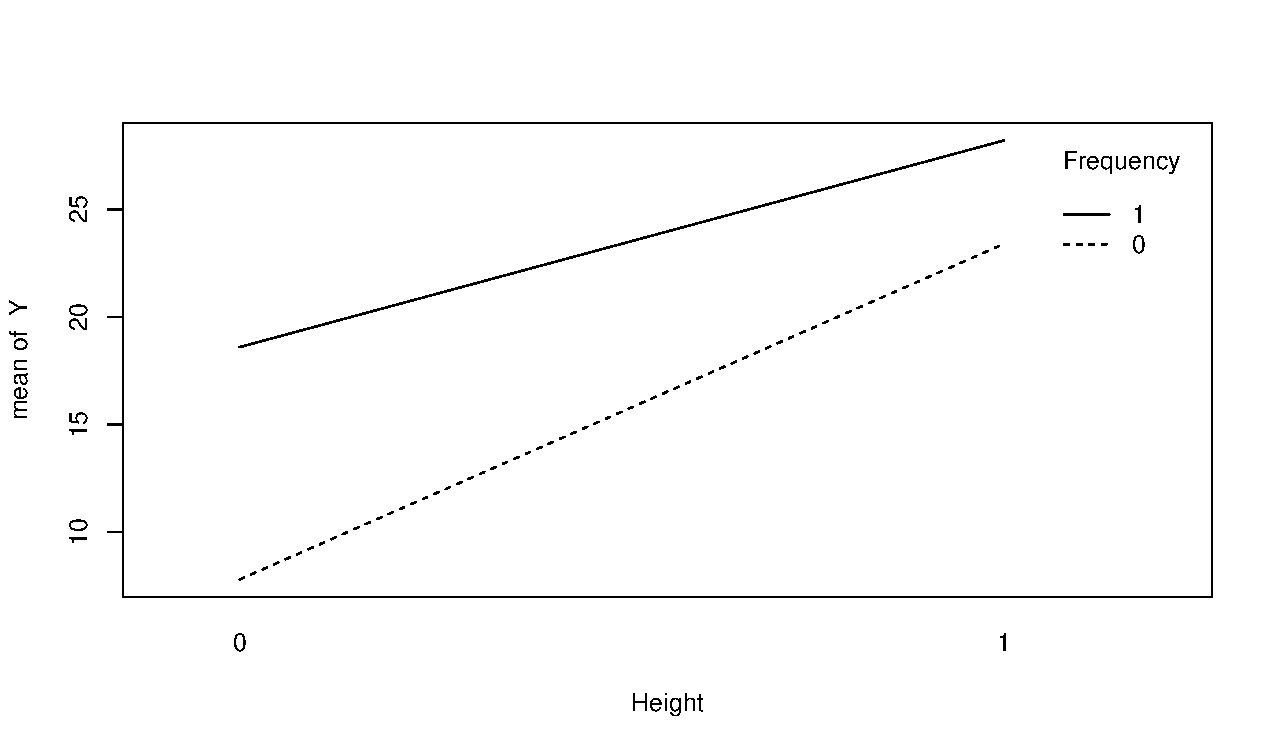
\includegraphics[width=\maxwidth]{figure/interplot-1} 

}

\caption[Interaction Plot]{Interaction Plot}\label{fig:interplot}
\end{figure}

\end{knitrout}
\subsection{Determining Interaction (Method 2)}
\begin{itemize}
    \item If $ \Delta_1=\Delta_2 $, the lines are parallel; that is, there is no interaction.
    \item If $ \Delta_1\ne \Delta_2 $, the lines are not parallel; that is, there is interaction.
\end{itemize}
$ \Delta_1-\Delta_2=(\bar{Y}_{11+}-\bar{Y}_{01+})-(\bar{Y}_{10+}-\bar{Y}_{00+}) $.
Add tildes to get $ \tilde{\theta}=(\tilde{\tau}_{11}-\tilde{\tau}_{01})-(\tilde{\tau}_{10}-\tilde{\tau}_{00}) $
\[ \E{\tilde{\theta}}=\tau_{11}-\tau_{01}-\tau_{10}-\tau_{00} \]
\[ \Var{\tilde{\theta}}=\frac{\sigma^2}{5} +\frac{\sigma^2}{5} +\frac{\sigma^2}{5} +\frac{\sigma^2}{5}
    =\frac{4\sigma^2}{5}  \]
$ H_0 $: $ \theta=0 $ (no interaction) versus $ H_a $: $ \theta\ne 0 $ (interaction)
\[ d=\frac{\hat{\tau}_{11}-\hat{\tau}_{01}-\hat{\tau}_{10}-\hat{\tau}_{00}}{\sigma\sqrt{\frac{4}{5}}}=-0.66\quad(D \sim t(20-4-1+1)=t(16)) \]
\[ p=2\Prob{D>0.66}=(0.4,0.6) \]
There is no evidence to reject $ H_0 $. Therefore, there is no interaction.

There is actually a \emph{third} way to determine interaction, the ANOVA table.
\subsection{Determining Interaction (Method 3)}
\begin{knitrout}
\definecolor{shadecolor}{rgb}{0.969, 0.969, 0.969}\color{fgcolor}\begin{kframe}
\begin{alltt}
\hlkwd{rm}\hlstd{(}\hlkwc{list} \hlstd{=} \hlkwd{ls}\hlstd{())}
\hlkwd{options}\hlstd{(}\hlkwc{contrasts} \hlstd{=} \hlkwd{c}\hlstd{(}\hlstr{"contr.sum"}\hlstd{,} \hlstr{"contr.poly"}\hlstd{))}
\hlstd{data} \hlkwb{=} \hlkwd{read.table}\hlstd{(}\hlstr{"stepping2.csv"}\hlstd{,} \hlkwc{header} \hlstd{= T,} \hlkwc{sep} \hlstd{=} \hlstr{","}\hlstd{,} \hlkwc{as.is} \hlstd{= T)}
\hlkwd{attach}\hlstd{(data)}
\hlstd{Y} \hlkwb{=} \hlstd{HR} \hlopt{-} \hlstd{RestHR}
\hlstd{Height} \hlkwb{=} \hlkwd{as.factor}\hlstd{(Height)}
\hlstd{Freq} \hlkwb{=} \hlkwd{as.factor}\hlstd{(Frequency)}
\hlstd{Model} \hlkwb{=} \hlkwd{lm}\hlstd{(Y} \hlopt{~} \hlstd{Freq} \hlopt{+} \hlstd{Height} \hlopt{+} \hlstd{Freq} \hlopt{*} \hlstd{Height)}
\hlkwd{anova}\hlstd{(Model)}
\end{alltt}
\begin{verbatim}
## Analysis of Variance Table
## 
## Response: Y
##             Df Sum Sq Mean Sq F value  Pr(>F)  
## Freq         1  304.2  304.20  2.9714 0.10401  
## Height       1  793.8  793.80  7.7538 0.01326 *
## Freq:Height  1   45.0   45.00  0.4396 0.51677  
## Residuals   16 1638.0  102.37                  
## ---
## Signif. codes:  0 '***' 0.001 '**' 0.01 '*' 0.05 '.' 0.1 ' ' 1
\end{verbatim}
\end{kframe}
\end{knitrout}
We calculate $ \SS{Trt} $ with
\[ \SS{Freq}+\SS{Height}+\SS{Interaction}=\SS{Trt} \]
In our case, $ \SS{Trt}=1143.0 $ on $ 3 $ degrees of freedom.
\begin{itemize}
    \item $ H_0 $: no interaction
    \item $ H_a $: interaction
\end{itemize}
\[ d=\frac{\MS{Int}}{\MS{Res}} =\frac{45}{102.37}=0.4396  \]
With $ p $-value,
\[ p=0.51667\quad(D \sim  F(1,16)) \]
$ p>0.1 $, so there is no evidence to reject $ H_0 $,
so it appears there is no interaction.

\chapter{Assignment 6}
\section{Lecture 31.00: Sampling}
Let
\begin{itemize}
    \item $ U $ be the \textbf{frame} (study population).
    \item $ U=\set{1,2,\ldots,N} $.
    \item $ \mathcal{S} $ be our sample. It has size $ n\le N $
          and $ \mathcal{S}\subset U $.
\end{itemize}
Also, let the \textbf{sampling protocol} refer
the probability of selecting any particular sample.
\begin{itemize}
    \item Define $ \pi_{ij} $ to be the \textbf{inclusion probability}
          for unit $ i $ and $ j $. (note: $ \pi_{ii}=\pi_{i} $)
\end{itemize}
\textbf{SRSWOR}
\begin{itemize}
    \item \underline{S}imple \underline{R}andom \underline{S}ampling \underline{w}ith\underline{o}ut
          \underline{R}eplacement.
    \item $ U=\set{1,2,3,4} $ we select samples of size $ n=2 $.
    \item $ \mathcal{S}_1=\set{1,2} $, $ \mathcal{S}_2=\set{1,3} $,
          $ \mathcal{S}_3=\set{1,4} $, $ \mathcal{S}_4=\set{2,3} $,
          $ \mathcal{S}_5=\set{2,4} $, $ \mathcal{S}_6=\set{3,4} $
    \item What is the probability we select sample 1?
          \[ \Prob{\mathcal{S}_1}=\frac{1}{6} \]
    \item What is the probability that unit 1 is in our sample?
          That is, what is $ \pi_1$? Well, $\pi_1=3/6=1/2 $.
\end{itemize}
Let the \textbf{frame} be $ \set{1,2,\ldots,N} $.
We select SRSWOR a sample of size $ n $.
\[ \Prob{\mathcal{S}_1}=\frac{1}{\binom{N}{n}} \]
\[ \pi_1=\frac{\binom{N-1}{n-1}}{\binom{N}{n}} =\frac{n}{N} \]
\section{Lecture 32.00: Model 1 Revisited}
\[ Y_{j}=\mu+R_j\quad(R_j \sim \N{0,\sigma^2}) \]
\begin{itemize}
    \item Parameters: $ \mu $, and $ \sigma^2 $
    \item Estimates: $ \hat{\mu}=\bar{y}_+ $, and $ \hat{\sigma}^2=s^2 $
    \item Estimators: $ \tilde{\mu}=\bar{Y}_+ $, and $ \tilde{\sigma}^2=S^2 $, where
          \[ \tilde{\mu} \sim \N*{\mu,\frac{\sigma^2}{n}} \]
    \item CI\@: $ \text{EST} \pm c\, \text{SE} $. For $ \mu $:
          \[ \hat{\mu}\pm c \frac{\hat{\sigma}}{\sqrt{n}} \quad(c \sim t(n-1)) \]
\end{itemize}
Use SRS (simple random sampling without replacement):
\begin{itemize}
    \item Parameters:
          \[ \mu=\frac{\sum_{i=1}^{N}y_i}{N} \]
          \[ \sigma^2=\frac{\sum_{i=1}^{N} (y_i-\mu)^2}{N-1}  \]
    \item Estimates:
          \[ \hat{\mu}=\frac{\sum_{i\in\mathcal{S}}y_i}{n}   \]
          \[ \hat{\sigma}^2=\frac{\sum_{i\in\mathcal{S}} (y_i-\hat{\mu})^2}{n-1}  \]
    \item Estimator: $ y_i $ is not a realization of $ Y_i $. Instead, $ y_i $ is a
          constant. What is random, is whether $ y_i $ is selected for the sample.
          \[ I_i=\begin{cases*}
                  0 & if $ y_i $ is not in the sample \\
                  1 & if $ y_i $ is in the sample
              \end{cases*} \]
          \[ \tilde{\mu}=\frac{\sum_{i=1}^{N} I_i y_i}{n} \]
          \[ \tilde{\sigma}^2=\frac{\sum_{i=1}^{N} I_i(y_i-\hat{\mu})^2}{n-1}  \]
          \[ \tilde{\mu}
              \sim \N*{\mu,\biggl(1-\frac{n}{N} \biggr)\frac{\sigma^2}{n}} \]
          where
          \begin{itemize}
              \item $ \dfrac{n}{N} $ is the sampling fraction
              \item $ 1-\dfrac{n}{N} $ is the finite population correction.
          \end{itemize}
\end{itemize}
\begin{table}[!htbp]
    \centering
    \begin{NiceTabular}{c|c}
        Model 1                                                        & SRS                                                                                  \\
        \midrule
        $ \displaystyle \hat{\mu}\pm c \frac{\hat{\sigma}}{\sqrt{n}} $ & $ \displaystyle \hat{\mu}\pm c \sqrt{1-\frac{n}{N} }\frac{\hat{\sigma}}{\sqrt{n}}  $
    \end{NiceTabular}
\end{table}
Let's prove the distribution.
\begin{itemize}
    \item $ \displaystyle \Prob{I_i=1}=\pi_i=\frac{n}{N} $
    \item $ \displaystyle \E{I_i}=(0)\Prob{I_i=0}+(1)\Prob{I_i=1}=\frac{n}{N}=\E{I_i^2} $
    \item $ \displaystyle \Var{I_i}=\E{I_i^2}-\E{I_i}^2=\frac{n}{N} -\biggl(\frac{n}{N}\biggr)^2=\frac{n}{N} \biggl(1-\frac{n}{N} \biggr)  $
    \item $ \displaystyle \E{I_i I_j}=(1)(1)\Prob{I_i=1,I_j=1}=\frac{\binom{N-2}{n-2}}{\binom{N}{n}}=\frac{n(n-1)}{N(N-1)}  $
\end{itemize}
Recall:
\[ \tilde{\mu}=\frac{\sum_{i=1}^{N} I_i y_i}{n} \]
\[ \E{\tilde{\mu}}=\frac{\sum_{i=1}^{N} \E{I_i}y_i}{n}=\frac{\sum_{i=1}^{N} (n/N) y_i}{n}=\mu  \]
We note that $ I_i $ is not independent of $ I_j $, so we must compute covariance in our variance calculation.
\[ \Var{\tilde{\mu}}=\Var*{\frac{\sum_{i=1}^{N} I_i y_i}{n}}=
    \frac{\sum_{i=1}^{N} y_i^2\Var{I_i}}{n^2}+\frac{\sum_{ij}y_i y_j\Cov{I_i,I_j}}{n^2}=
    \biggl(1-\frac{n}{N} \biggr)\frac{\sigma^2}{n}   \]

\section{Lecture 33.00: Sample Size Calculation}
\underline{Model 1}:
$ \displaystyle  \hat{\mu}\pm \frac{c\sigma}{\sqrt{n}} $ where $\sigma$ is known.

Set $ E=\displaystyle \frac{c\sigma}{\sqrt{n}} $ and solve for $ n $. Therefore,
$ \displaystyle n=\frac{c^2\sigma^2}{E^2} $.

\underline{Process}
\begin{itemize}
    \item First, we take a small sample, then estimate $ \sigma $.
    \item Find $ n $.
    \item Perform a large study with $ n $ units.
\end{itemize}
For SRS for our mean we have:
\[ \hat{\mu}\pm \Uunderbracket{\frac{c\hat{\sigma}}{\sqrt{n}}\sqrt{1-\frac{n}{N}}}_{E} \]
\[ n=\biggl(\frac{E^2}{c^2\hat{\sigma}^2}+\frac{1}{N} \biggr)^{\!-1} \]
\begin{Example}{SRSWOR Example 1}{}
    \textbf{Part 1}. Assume our class has 200 students in it.
    I draw a sample of 5 students to find the average on
    midterm 2 is 65\% with a standard deviation of 3\%.
    Build a 95\% confidence interval for $ \mu $. Please assume
    that $ n $ is ``large'' enough to apply the normality assumption.

    \textbf{Solution.}
    \begin{align*}
         & \hat{\mu}\pm \frac{c\hat{\sigma}}{\sqrt{n}}\sqrt{1-\frac{n}{N}}\quad c\sim \N{0,1} \\
         & =65\pm \frac{1.96(3)}{\sqrt{5}} \sqrt{1-\frac{5}{200} }                            \\
         & =(0.62,0.68)
    \end{align*}
    The width is $ 0.68-0.62\approx 0.06 $.

    \textbf{Part 2}.
    If I want to be accurate to within 0.1, 19 times out of 20 how large should $n$ be?
    \begin{itemize}
        \item $ E=0.1 $.
        \item $ \frac{19}{20} =0.95\implies 95\% $.
        \item $ \sigma=3 $.
        \item $ \mu=65 $.
    \end{itemize}
    SRS\@:
    \[ n=\biggl(\frac{E^2}{c^2\hat{\sigma}^2}+\frac{1}{N}  \biggr)^{\!-1}
        =\biggl(\frac{0.1^2}{1.96^2 3^2}+\frac{1}{200} \biggr)^{\!-1}=189.0634=\;\uparrow 190 \]
    \underline{Model 1}: Assumes $ N\to \infty $.
    \[ n=\frac{c^2\hat{\sigma}^2}{E^2}=3457.44=\;\uparrow 3458  \]
\end{Example}
\section{Lecture 34.00: Model 4 Revisited}
\underline{Model 4}: $ \displaystyle \frac{Y_i}{n} \sim \N*{\pi,\frac{\pi(1-\pi)}{n} } $
with confidence interval:
\[ \pi:\hat{\pi}\pm c\sqrt{\frac{\hat{\pi}(1-\hat{\pi})}{n} } \]
\subsection*{SRS for $ \pi $}
\begin{itemize}
    \item SP Parameter:
          \[ \pi=\frac{\sum_{i=1}^{N} y_i}{N}\quad(y_i=\set{0,1}) \]
    \item Statistic:
          \[ \hat{\pi}=\frac{\sum_{i\in\mathcal{S}}y_i }{n}=\bar{y}  \]
          \[ \hat{\sigma}^2=\frac{\sum_{i\in\mathcal{S}}(y_i-\bar{y})^2}{n-1}=
              \frac{\sum_{i\in\mathcal{S}}(y_i^2+\bar{y}^2-2y_i\bar{y})}{n-1}    \]
          Recall that $ y_i=\set{0,1} $. Therefore,
          \[ \hat{\sigma}^2=
              \frac{\sum_{i\in\mathcal{S}}(y_i+\bar{y}^2-2y_i\bar{y})}{n-1}
              =\frac{n\bar{y}+n\bar{y}^2-2\bar{y}n\bar{y}}{n-1}
              =\frac{n}{n-1} (\bar{y}-\bar{y}^2)=\frac{n}{n-1} \bigl[\hat{\pi}(1-\hat{\pi})\bigr]  \]
          since $ \bar{y}=\hat{\pi} $. Now, assume that $ n\to\infty $. Therefore,
          \[ \hat{\sigma}^2=\hat{\pi}(1-\hat{\pi}) \]
    \item Estimators:
          \[ \tilde{\pi}=\frac{\sum_{i=1}^{N} y_i I_i}{n} \]
          \begin{Exercise}{}{}
              In SRS, clearly show that $ \tilde{\pi} $ is an unbiased estimator for $ \pi $.

              \textbf{Solution.} In SRS, $\tilde{\pi}$ is defined by:
              \[ \tilde{\pi}=\frac{\sum_{i=1}^N y_i I_i}{n}\quad\text{where}\quad I_i =\begin{cases}
                      1 & \text{if $y_i$ is in the sample}     \\
                      0 & \text{if $y_i$ is not in the sample}
                  \end{cases}\quad \text{and}\quad y_i=0\text{ or }1. \]
              In \texttt{Lec 32.00: Model 1 Revisited},
              we derived that $\E{I_i}=n/N$.
              Hence,
              \[
                  \E*{\tilde{\pi}}
                  =\E*{\frac{\sum_{i=1}^N y_i I_i}{n}}
                  =\frac{\sum_{i=1}^N y_i\E{I_i}}{n}
                  =\frac{\sum_{i=1}^N y_i(n/N)}{n}
                  =\frac{\sum_{i=1}^N y_i}{N}
                  =\pi
              \]
              Therefore, in SRS $\tilde{\pi}$ is an unbiased estimator for $\pi$.
          \end{Exercise}
          \begin{Remark}{}{}
              $ \tilde{\pi} $ is normal.
          \end{Remark}
          \[
              \Var{\tilde{\pi}}
              =\Var*{\frac{\sum_{i=1}^{N} y_i I_i}{n}}
              =\cdots
              =\frac{\sigma^2}{n} \biggl(1-\frac{n}{N}\biggr)
          \]
          Replace $ \sigma $ by $ \hat{\sigma}^2=\hat{\pi}(1-\hat{\pi}) $.
          Our confidence interval is:
          \[ \hat{\pi}\pm c\sqrt{\frac{\hat{\pi}(1-\hat{\pi})}{n}\biggl(1-\frac{n}{N}\biggr)} \]
          \underline{Model 4}:
          \[ \hat{\pi}\pm c\sqrt{\frac{\hat{\pi}(1-\hat{\pi})}{n}} \]
\end{itemize}
\subsection*{Sample Size Calculation}
\[ n=\biggl(\frac{E^2}{\sigma^2c^2} +\frac{1}{N} \biggr)^{\!-1} \]
However, $ \hat{\sigma}^2=\hat{\pi}(1-\hat{\pi}) $. Often,
we replace $ \hat{\sigma}^2 $ by $ 1/4 $ which is the maximum.

\section{Lecture 35.00: SRS Examples}
\begin{Example}{SRSWOR Example 2}{}
    According to a new poll conducted by Ipsos Reid
    on behalf of Postmedia News and Global Television,
    $42\%$, `approve' of the performance of the Conservative
    government under the leadership of Stephen
    Harper. For this survey, a sample of $1053$ Canadians,
    from Ipsos' Canadian online panel was interviewed online.
    This result is $3\%$ lower than last years' results.

    Is the difference between this year and last years' results significant;
    that is, is there a difference? Use a
    confidence interval with a $95\%$ level of confidence to answer the question.

    \textbf{Solution.}
    \[ \hat{\pi}\pm c\sqrt{\frac{\hat{\pi}(1-\hat{\pi})}{n}}=0.42\pm 1.96\sqrt{\frac{0.42(1-0.42)}{1053}}
        =(0.39,0.45) \]
    Now, $ 0.45 $ is in the interval (it's at the edge which is fine for
    our purposes), so there is no difference between
    this year and last years' results; that is, they are the same.
\end{Example}
\begin{Example}{SRSWOR Example 3}{}
    Jeff Henry, a counsellor for Waterloo wants to know how many people
    he should poll so that with $95\%$
    confidence his poll (``will you vote for me?''),
    is accurate with a margin of error of 1\%. There are $150\,000$
    people in his Waterloo riding.

    \textbf{Solution.}
    \begin{itemize}
        \item $ c=1.96 $.
        \item $ E=0.01 $.
        \item $ N=150\,000 $.
        \item We should assume the worst-case scenario for the proportion;
              that is, $ \hat{\pi}=1/2 $.
        \item $ \hat{\sigma}^2=\hat{\pi}(1-\hat{\pi}) $.
    \end{itemize}
    \[ n=\biggl(\frac{E^2}{\hat{\sigma}^2c^2}+\frac{1}{N} \biggr)^{\!-1}
        =9026.09=\;\uparrow 9027 \]
\end{Example}
\begin{Example}{SRSWOR Example 4}{}
    Sheila is an auditor.
    She has taken a sample of $15$ accounts across a large company
    to see whether the company is being compliant
    (i.e., following accounting laws). In these she has found that the
    amount of misstated account values is, on average, $\$143.95$.
    The variance of her sample values is $\$81.09$. If there are a total
    of $200$ accounts to look at, and her auditing company allows a level of
    non-compliance up to $\$25\,000$ dollars, then is this company being compliant?
    Make your decision at a 90\% level of confidence.

    \textbf{Solution.}
    \begin{itemize}
        \item $ c=1.645 $.
        \item $ \hat{\mu}=143.95 $.
        \item $ \hat{\sigma}^2=81.09 $.
        \item $ N=200 $.
        \item $ n=15 $.
    \end{itemize}
    \[ \hat{\mu}\pm \frac{c\hat{\sigma}}{\sqrt{n}}\sqrt{1-\frac{n}{N}}=(140.27,147.63) \]
    On \underline{average} the discrepancy is $(140.27,147.63)$ with $90\%$ confidence.
    However,
    \[ 200(140.27,147.63)=(28\,054,29\,526)>25\,000 \]
    We can say that the company is not being compliant.
\end{Example}


\chapter{Assignment 7}
\section{Lecture 36.00: Regression Sampling}
We want our parameter to be
\[ \mu_y = \frac{\sum_{i=1}^{N} y_i}{N}  \]
which is our population average.

We use
\[ \hat{\mu}_y=\frac{\sum_{i\in\mathcal{S}}y_i}{n}=\bar{y}  \]
which is our sample average.

Suppose $ Y_i $ is linearly related to a \emph{continuous}
explanatory variate called $ x_i $. If that's the case,
$ x_i $ has its own population average
\[ \mu_x= \frac{\sum_{i=1}^{N} x_i}{N} \]
with sample mean
\[ \hat{\mu}_x=\frac{\sum_{i\in\mathcal{S}} x_i }{n}=\bar{x}  \]
Suppose we have a linear relationship of the form
$ Y_i=\alpha+\beta(x_i-\bar{x})+R_i $ where $ R_i \sim \N{0,\sigma^2} $.

We use least squares,
\[ W=\sum_{i}r_i^2=\sum_{i}\bigl[y_i-\alpha-\beta(x_i-\bar{x})\bigr]^2  \]
We find $\pd{W}{\alpha}$ and $\pd{W}{\beta}$, and you can show this for homework:
\begin{align*}
    \hat{\alpha} & =\bar{y}                                                                                                \\
    \hat{\beta}  & =\frac{\sum_{i}y_i(x_i-\bar{x})}{\sum_{i}(x_i-\bar{x})^2 }=\frac{S_{xy}}{S_{xx}}=\frac{s_{xy}}{s_{x}^2}
\end{align*}
where
\begin{align*}
    S_{xy}  & =\sum_{i}y_i(x_i-\bar{x})=\sum_{i}(y_i-\bar{y})(x_i-\bar{x}) \\
    s_{xy}  & =\frac{S_{xy}}{n-1}                                          \\
    S_{xx}  & =\sum_{i}(x_i-\bar{x})^2                                     \\
    s_{x}^2 & =\frac{S_{xx}}{n-1}
\end{align*}
We had $ y_i=\alpha+\beta(x_i-\bar{x})+R_i $. We used least squares
to estimate $ \alpha $ and $ \beta $ to obtain (ignoring the $ R_i $ term)
\[ \hat{y}_i=\hat{\alpha}+\hat{\beta}(x_i-\bar{x}) \]
\begin{itemize}
    \item If $ x_i=\bar{x} $, then $ \hat{y}_i=\hat{\alpha}=\bar{y} $.
    \item If $ x_i=\mu_x $, then $ \hat{y}_i=\hat{\alpha}+\hat{\beta}(\mu_x-\bar{x})=\hat{\mu}_{\text{reg}} $.
\end{itemize}
\[ \boxed{\hat{\mu}_{\text{reg}}=\hat{\alpha}+\hat{\beta}(\mu_x-\bar{x})} \]
\subsection*{Estimators}
The $ \alpha,\beta,\mu_x,\mu_y $ estimators are all unbiased. However,
\begin{align*}
    \hat{\mu}_{\text{reg}}
     & =\hat{\alpha}+\hat{\beta}(\mu_x-\bar{x})                                                                              \\
     & =\hat{\alpha}-\hat{\beta}(\bar{x}-\mu_x)                                                                              \\
     & =\bar{y}-\hat{\beta}(\bar{x}-\mu_x)                                                                                   \\
     & =\frac{\sum_{i\in\mathcal{S}}y_i}{n}-\hat{\beta}\biggl(\frac{\sum_{i\in\mathcal{S}}x_i }{n}-\frac{n\mu_x}{n}  \biggr) \\
     & =\frac{\sum_{i\in\mathcal{S}}\bigr[y_i-\hat{\beta}(x_i-\mu_x)\bigl]}{n}                                               \\
     & =\frac{\sum_{i\in\mathcal{S}}r_i }{n}
\end{align*}
\[ \tilde{\mu}_{\text{reg}}=\frac{\sum_{i=1}^{N} I_i r_i}{n} \]
We're interested in three things for $ \tilde{\mu}_{\text{reg}} $:
\begin{itemize}
    \item Distribution. We're not going into the details, but
          we get that $ \tilde{\mu}_{\text{reg}} $ is normally distributed.
    \item Expected Value.
    \item Variance.
\end{itemize}
\subsection*{Expected Value and Variance of $ \tilde{\mu}_{\text{reg}} $}
\begin{align*}
    \E*{\tilde{\mu}_{\text{reg}}}
     & =\E*{\tilde{\alpha}+\tilde{\beta}(\tilde{\mu}_x-\mu_x)}                       \\
     & =\E*{\tilde{\mu}_y+\tilde{\beta}(\tilde{\mu}_x-\mu_x)}                        \\
     & =\mu_y+\Uunderbracket{\E*{\tilde{\beta}(\tilde{\mu}_x-\mu_x)}}_{\text{small}}
\end{align*}
Therefore, $ \tilde{\mu}_{\text{reg}} $ is a \underline{biased} estimator for $ \mu_y $.
\begin{align*}
    \Var*{\tilde{\mu}_{\text{reg}}}
     & =\Var*{\frac{\sum_{i=1}^{N} I_i r_i}{n} }        \\
     & =\biggl(1-\frac{n}{N}\biggr)\frac{\sigma_r^2}{n}
\end{align*}
We estimate $ \sigma_r^2 $ by
\[ \hat{\sigma}_r^2=\frac{\sum_{i\in\mathcal{S}}(r_i-\bar{r})^2}{n-1}=\cdots=\frac{W}{n-1}  \]
The confidence interval is:
\[ \hat{\mu}_{\text{reg}}\pm c\sqrt{1-\frac{n}{N}}\frac{\hat{\sigma}_r}{\sqrt{n}}  \]


\section{Lecture 37.00: Regression Sampling, Example}
\begin{itemize}
    \item In R the data set is \code{women}. Simply type \code{women} to see the data.
    \item We assume this is our population and that we want to know the mean height $\mu_{\text{height}}$.
    \item When you do regression sampling you need to have a $y$ and an $x$.
    \item $y$: height.
    \item $x$: weight.
    \item Now when we talk about our $x$ being weight we have to assume that we know the mean weight $\mu_{\text{weight}}$; that is, you need to know the population value for your weight. You don't know your population value for your height that's what you're trying to build the interval about.
\end{itemize}
\begin{knitrout}
\definecolor{shadecolor}{rgb}{0.969, 0.969, 0.969}\color{fgcolor}\begin{kframe}
\begin{alltt}
\hlkwd{attach}\hlstd{(women)}
\hlkwd{mean}\hlstd{(height)}
\end{alltt}
\begin{verbatim}
## [1] 65
\end{verbatim}
\begin{alltt}
\hlkwd{mean}\hlstd{(weight)}
\end{alltt}
\begin{verbatim}
## [1] 136.7333
\end{verbatim}
\end{kframe}
\end{knitrout}
\begin{itemize}
    \item $\mu_{\text{height}}=65$ is unknown!
    \item $\mu_{\text{weight}}\approx 136.7333$ is known, and must be known to do regression sampling.
\end{itemize}

We're almost there where we have everything we need. Once we get everything we need,
we can build an SRS confidence interval. We need one more thing, and that's getting
a sample. The sample command below grabs five \code{height}s from the set of heights
that are there. So it grabs five of them, and then we can get the mean of the sample height
and the standard deviation of the sample heights, so this would be sigma hat for simple random sampling.

Using SRSWOR, we take a sample of size $5$ and use this as our estimate for the height.

\begin{knitrout}
\definecolor{shadecolor}{rgb}{0.969, 0.969, 0.969}\color{fgcolor}\begin{kframe}
\begin{alltt}
\hlkwd{set.seed}\hlstd{(}\hlnum{45376}\hlstd{)}
\hlstd{sample_heights} \hlkwb{=} \hlkwd{sample}\hlstd{(height,} \hlnum{5}\hlstd{)}
\hlkwd{mean}\hlstd{(sample_heights)}
\end{alltt}
\begin{verbatim}
## [1] 63.4
\end{verbatim}
\begin{alltt}
\hlkwd{sd}\hlstd{(sample_heights)}
\end{alltt}
\begin{verbatim}
## [1] 3.209361
\end{verbatim}
\end{kframe}
\end{knitrout}
\begin{itemize}
    \item $\hat{\mu}_{\text{height}}=63.4$.
    \item $\hat{\sigma}_{\text{SRS}}\approx 3.209361$.
\end{itemize}

Now we have enough information that we can actually build a confidence interval.

\begin{knitrout}
\definecolor{shadecolor}{rgb}{0.969, 0.969, 0.969}\color{fgcolor}\begin{kframe}
\begin{alltt}
\hlstd{N} \hlkwb{<-} \hlkwd{nrow}\hlstd{(women)}
\hlkwd{print}\hlstd{(N)}
\end{alltt}
\begin{verbatim}
## [1] 15
\end{verbatim}
\begin{alltt}
\hlstd{n} \hlkwb{<-} \hlnum{5}
\hlstd{c} \hlkwb{<-} \hlkwd{qnorm}\hlstd{(}\hlnum{0.975}\hlstd{)}
\hlkwd{round}\hlstd{(}\hlkwd{mean}\hlstd{(sample_heights)} \hlopt{+} \hlkwd{c}\hlstd{(}\hlopt{-}\hlnum{1}\hlstd{,} \hlnum{1}\hlstd{)} \hlopt{*} \hlstd{((c} \hlopt{*} \hlkwd{sd}\hlstd{(sample_heights))}\hlopt{/}\hlkwd{sqrt}\hlstd{(n))} \hlopt{*}
  \hlkwd{sqrt}\hlstd{(}\hlnum{1} \hlopt{-} \hlstd{n}\hlopt{/}\hlstd{N),} \hlnum{1}\hlstd{)}
\end{alltt}
\begin{verbatim}
## [1] 61.1 65.7
\end{verbatim}
\end{kframe}
\end{knitrout}
\begin{itemize}
    \item $N=15$.
    \item $n=5$.
    \item $c\approx 1.96$.
\end{itemize}

$$\text{SRS: }\hat{\mu}_\text{height}\pm \frac{c\hat{\sigma}_{\text{SRS}}}{\sqrt{n}}\sqrt{1-\frac{n}{N}}=63.4\pm \frac{1.96(3.209361)}{\sqrt{5}}\sqrt{1-\frac{5}{15}}=(61.1,65.7)$$
which has a width of $4.6$.


\begin{knitrout}
\definecolor{shadecolor}{rgb}{0.969, 0.969, 0.969}\color{fgcolor}\begin{kframe}
\begin{alltt}
\hlstd{sample_weights} \hlkwb{=} \hlkwd{c}\hlstd{(}\hlnum{123}\hlstd{,} \hlnum{129}\hlstd{,} \hlnum{135}\hlstd{,} \hlnum{146}\hlstd{,} \hlnum{120}\hlstd{)}
\hlkwd{mean}\hlstd{(sample_weights)}
\end{alltt}
\begin{verbatim}
## [1] 130.6
\end{verbatim}
\end{kframe}
\end{knitrout}
\begin{itemize}
    \item $\hat{\mu}_{\text{weight}}=130.6$.
\end{itemize}

We are wrong by $\mu_y-\hat{\mu}_y=65-63.4=1.6$ units. We note that
there is a linear relationship between height and weight.

\begin{knitrout}
\definecolor{shadecolor}{rgb}{0.969, 0.969, 0.969}\color{fgcolor}\begin{kframe}
\begin{alltt}
\hlkwd{plot}\hlstd{(weight, height)}
\end{alltt}
\end{kframe}

{\centering 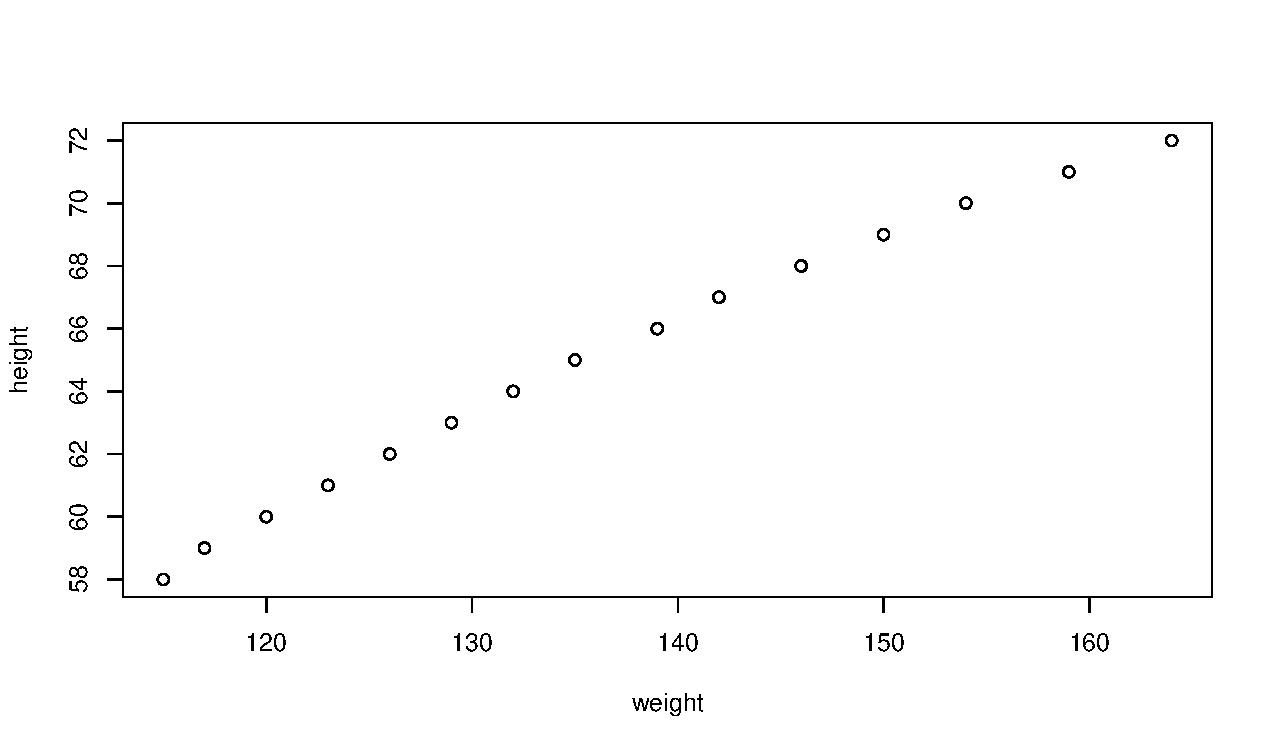
\includegraphics[width=\maxwidth]{figure/unnamed-chunk-33-1} 

}


\end{knitrout}

Thus, we decide to use Regression Sampling.

\begin{knitrout}
\definecolor{shadecolor}{rgb}{0.969, 0.969, 0.969}\color{fgcolor}\begin{kframe}
\begin{alltt}
\hlstd{sample_weights} \hlkwb{=} \hlstd{sample_weights} \hlopt{-} \hlkwd{mean}\hlstd{(sample_weights)}  \hlcom{# x_i - bar(x)}
\hlkwd{summary}\hlstd{(}\hlkwd{lm}\hlstd{(sample_heights} \hlopt{~} \hlstd{sample_weights))}  \hlcom{# Y_i ~ (x_i - bar(x))}
\end{alltt}
\begin{verbatim}
## 
## Call:
## lm(formula = sample_heights ~ sample_weights)
## 
## Residuals:
##        1        2        3        4        5 
## -0.04846  0.09506  0.23858 -0.16496 -0.12022 
## 
## Coefficients:
##                 Estimate Std. Error t value Pr(>|t|)    
## (Intercept)    63.400000   0.085624  740.45 5.43e-09 ***
## sample_weights  0.309413   0.009242   33.48 5.86e-05 ***
## ---
## Signif. codes:  0 '***' 0.001 '**' 0.01 '*' 0.05 '.' 0.1 ' ' 1
## 
## Residual standard error: 0.1915 on 3 degrees of freedom
## Multiple R-squared:  0.9973,	Adjusted R-squared:  0.9964 
## F-statistic:  1121 on 1 and 3 DF,  p-value: 5.858e-05
\end{verbatim}
\end{kframe}
\end{knitrout}
We didn't use a factor because this is not a discrete variable.
We consider this factor to be continuous, so we consider our weights to be a continuous value.

Therefore,

\begin{itemize}
    \item $\hat{\alpha}=\hat{\mu}_y=63.4$.
    \item $\hat{\beta}=0.309413$.
\end{itemize}

Right now, the degrees of freedom is $n-2=5-2=3$, but we want to multiply by $(n-2)/(n-1)$ as
the degrees of freedom should be $n-1=5-1=4$, so
\begin{knitrout}
\definecolor{shadecolor}{rgb}{0.969, 0.969, 0.969}\color{fgcolor}\begin{kframe}
\begin{alltt}
\hlstd{sigma_r} \hlkwb{<-} \hlkwd{summary}\hlstd{(}\hlkwd{lm}\hlstd{(}\hlkwc{formula} \hlstd{= sample_heights} \hlopt{~} \hlstd{sample_weights))}\hlopt{$}\hlstd{sigma}
\hlkwd{print}\hlstd{(sigma_r)}
\end{alltt}
\begin{verbatim}
## [1] 0.1914611
\end{verbatim}
\begin{alltt}
\hlstd{sigma_r_sq} \hlkwb{<-} \hlstd{sigma_r}\hlopt{^}\hlnum{2} \hlopt{*} \hlstd{(n} \hlopt{-} \hlnum{2}\hlstd{)}\hlopt{/}\hlstd{(n} \hlopt{-} \hlnum{1}\hlstd{)}
\hlkwd{print}\hlstd{(sigma_r_sq)}
\end{alltt}
\begin{verbatim}
## [1] 0.02749301
\end{verbatim}
\end{kframe}
\end{knitrout}
$$\hat{\sigma}_r^2=\hat{\sigma}_{\text{r}}^2\frac{3}{4}=0.1915^2(3/4)=0.02749$$

$$\hat{\mu}_{\text{reg}}=\hat{\mu}_{\text{height}}=\hat{\alpha}+\hat{\beta}(x_i-\bar{x})=63.4-0.31(x_i-130.6)$$
\begin{knitrout}
\definecolor{shadecolor}{rgb}{0.969, 0.969, 0.969}\color{fgcolor}\begin{kframe}
\begin{alltt}
\hlstd{alpha_hat} \hlkwb{<-} \hlkwd{summary}\hlstd{(}\hlkwd{lm}\hlstd{(}\hlkwc{formula} \hlstd{= sample_heights} \hlopt{~} \hlstd{sample_weights))}\hlopt{$}\hlstd{coefficients[}\hlnum{1}\hlstd{]}
\hlstd{beta_hat} \hlkwb{<-} \hlkwd{summary}\hlstd{(}\hlkwd{lm}\hlstd{(}\hlkwc{formula} \hlstd{= sample_heights} \hlopt{~} \hlstd{sample_weights))}\hlopt{$}\hlstd{coefficients[}\hlnum{2}\hlstd{]}
\hlstd{reg} \hlkwb{<-} \hlkwd{mean}\hlstd{(sample_heights)} \hlopt{+} \hlstd{beta_hat} \hlopt{*} \hlstd{(}\hlkwd{mean}\hlstd{(weight)} \hlopt{-} \hlkwd{mean}\hlstd{(}\hlkwd{c}\hlstd{(}\hlnum{123}\hlstd{,}
  \hlnum{129}\hlstd{,} \hlnum{135}\hlstd{,} \hlnum{146}\hlstd{,} \hlnum{120}\hlstd{)))}
\hlkwd{print}\hlstd{(reg)}
\end{alltt}
\begin{verbatim}
## [1] 65.29773
\end{verbatim}
\end{kframe}
\end{knitrout}
The regression estimate is:
$$\hat{\mu}_{\text{reg}}=\hat{\mu}_{\text{height}}(\mu_{\text{weight}})=63.4+0.31(136.7333-130.6)=65.3$$
\begin{knitrout}
\definecolor{shadecolor}{rgb}{0.969, 0.969, 0.969}\color{fgcolor}\begin{kframe}
\begin{alltt}
\hlkwd{round}\hlstd{(reg} \hlopt{+} \hlkwd{c}\hlstd{(}\hlopt{-}\hlnum{1}\hlstd{,} \hlnum{1}\hlstd{)} \hlopt{*} \hlstd{c} \hlopt{*} \hlkwd{sqrt}\hlstd{(sigma_r_sq)}\hlopt{/}\hlkwd{sqrt}\hlstd{(}\hlnum{5}\hlstd{)} \hlopt{*} \hlstd{(}\hlnum{1} \hlopt{-} \hlstd{n}\hlopt{/}\hlstd{N),}
  \hlnum{1}\hlstd{)}
\end{alltt}
\begin{verbatim}
## [1] 65.2 65.4
\end{verbatim}
\end{kframe}
\end{knitrout}
The confidence interval is:
$$\hat{\mu}_{\text{reg}}\pm \frac{c\hat{\sigma}_r}{\sqrt{n}}\sqrt{1-\frac{n}{N}}=65.3\pm \frac{1.96\sqrt{0.02749}}{\sqrt{5}}\sqrt{1-\frac{5}{15}}=(65.2,65.4)$$
In this case, you are only $0.3$ from the true mean.

\begin{itemize}
    \item The width of this interval is much narrower than that of the SRS.
          In fact, for the SRS if we go back in time it had a width of 4.6.
    \item Note that your interval does not actually contain the population mean height.
          The population mean height is $65$, but it's not in your interval and that's
          because of the bias that comes from a regression interval. So, the bias of a regression
          interval means that we may not always
          contain the actual value of interest. You won't be far off from it because of
          the regression line, but your interval might not contain it.
\end{itemize}

\begin{knitrout}
\definecolor{shadecolor}{rgb}{0.969, 0.969, 0.969}\color{fgcolor}\begin{kframe}
\begin{alltt}
\hlkwd{plot}\hlstd{(weight, height)}
\hlkwd{abline}\hlstd{(}\hlkwc{h} \hlstd{=} \hlkwd{mean}\hlstd{(height))}
\hlkwd{abline}\hlstd{(}\hlkwc{v} \hlstd{=} \hlkwd{mean}\hlstd{(weight))}
\hlkwd{abline}\hlstd{(alpha_hat} \hlopt{-} \hlstd{beta_hat} \hlopt{*} \hlkwd{mean}\hlstd{(}\hlkwd{c}\hlstd{(}\hlnum{123}\hlstd{,} \hlnum{129}\hlstd{,} \hlnum{135}\hlstd{,} \hlnum{146}\hlstd{,} \hlnum{120}\hlstd{)),}
  \hlstd{beta_hat)}
\end{alltt}
\end{kframe}

{\centering 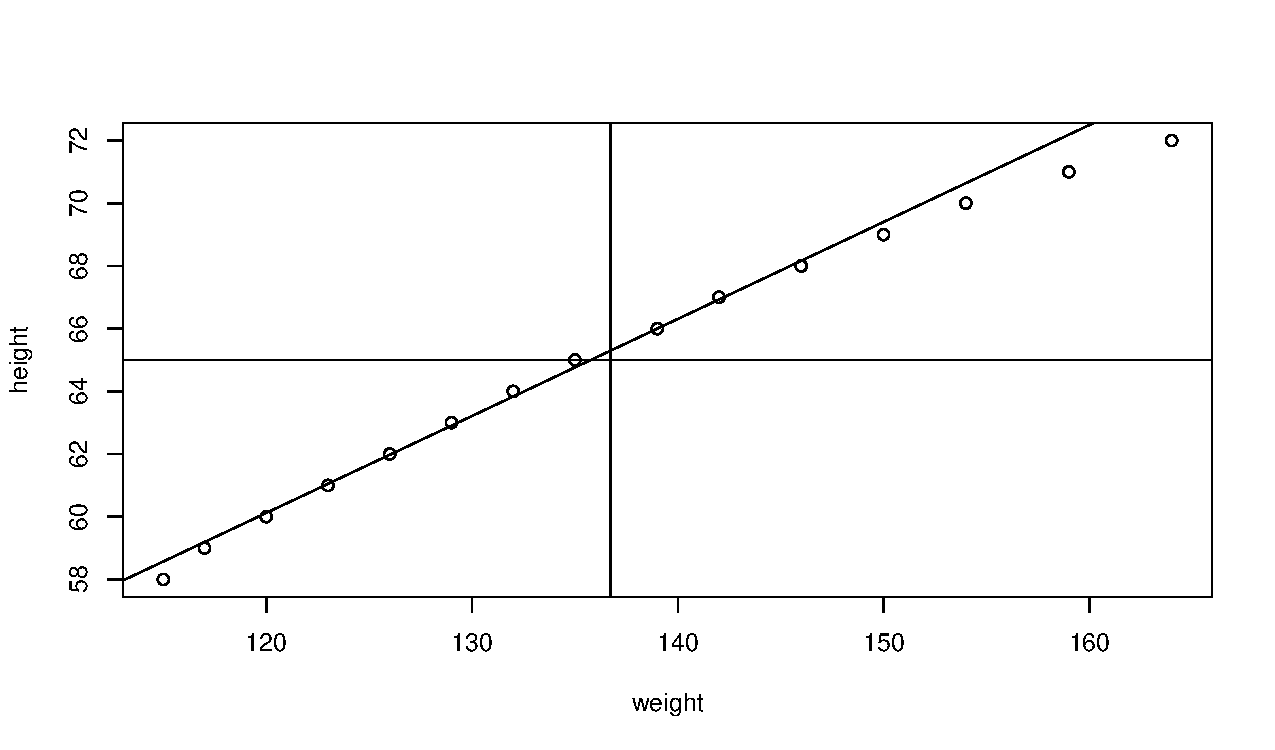
\includegraphics[width=\maxwidth]{figure/unnamed-chunk-38-1} 

}


\end{knitrout}

\section{Lecture 38.00: Regression Sampling, Example 2}
A student was curious about whether they performed better with
more sleep. To test this hypothesis, she decided to write
various tests on a certain number of hours ($x$) of sleep.
The grade on their test was considered to be the response ($y$).
In total, she has written $94$ tests since coming to UW.
On average, she slept for $5.1$ hours during those $94$
tests. We consider the $9$ below to be a random sample.
\begin{itemize}
    \item \textbf{Model}: $Y_i=\alpha+\beta(x_i-\bar{x})+R_i$ where $R_i \sim \mathcal{N}(0,\sigma^2)$.
\end{itemize}
\textbf{Questions}:
\begin{itemize}
    \item Assume the explanatory variate was not present. Build a 95% confidence
          interval for her mean grade using SRSWOR.
    \item Use Regression sampling to build a 95% confidence interval for her mean grade.
    \item Compare your SRSWOR results to your regression results, what do you notice?
\end{itemize}

\begin{knitrout}
\definecolor{shadecolor}{rgb}{0.969, 0.969, 0.969}\color{fgcolor}\begin{kframe}
\begin{alltt}
\hlstd{x} \hlkwb{<-} \hlkwd{c}\hlstd{(}\hlnum{4}\hlstd{,} \hlnum{6}\hlstd{,} \hlnum{2}\hlstd{,} \hlnum{7}\hlstd{,} \hlnum{5}\hlstd{,} \hlnum{9}\hlstd{,} \hlnum{2}\hlstd{,} \hlnum{1}\hlstd{,} \hlnum{8}\hlstd{)}
\hlstd{y} \hlkwb{<-} \hlkwd{c}\hlstd{(}\hlnum{75}\hlstd{,} \hlnum{78}\hlstd{,} \hlnum{69}\hlstd{,} \hlnum{80}\hlstd{,} \hlnum{77}\hlstd{,} \hlnum{82}\hlstd{,} \hlnum{65}\hlstd{,} \hlnum{55}\hlstd{,} \hlnum{85}\hlstd{)}
\hlstd{n} \hlkwb{<-} \hlnum{9}
\hlstd{N} \hlkwb{<-} \hlnum{94}
\hlstd{mu_x} \hlkwb{<-} \hlnum{5.1}
\hlstd{s_xy} \hlkwb{<-} \hlkwd{sum}\hlstd{(y} \hlopt{*} \hlstd{(x} \hlopt{-} \hlkwd{mean}\hlstd{(x)))}\hlopt{/}\hlstd{(n} \hlopt{-} \hlnum{1}\hlstd{)}
\hlkwd{print}\hlstd{(s_xy)}
\end{alltt}
\begin{verbatim}
## [1] 24.75
\end{verbatim}
\begin{alltt}
\hlstd{s_xsq} \hlkwb{<-} \hlkwd{var}\hlstd{(x)}
\hlkwd{print}\hlstd{(s_xsq)}
\end{alltt}
\begin{verbatim}
## [1] 8.111111
\end{verbatim}
\begin{alltt}
\hlstd{s_ysq} \hlkwb{<-} \hlkwd{var}\hlstd{(y)}
\hlkwd{print}\hlstd{(s_ysq)}
\end{alltt}
\begin{verbatim}
## [1] 89.25
\end{verbatim}
\begin{alltt}
\hlstd{xbar} \hlkwb{<-} \hlkwd{mean}\hlstd{(x)}
\hlkwd{print}\hlstd{(xbar)}
\end{alltt}
\begin{verbatim}
## [1] 4.888889
\end{verbatim}
\begin{alltt}
\hlstd{ybar} \hlkwb{<-} \hlkwd{mean}\hlstd{(y)}
\hlkwd{print}\hlstd{(ybar)}
\end{alltt}
\begin{verbatim}
## [1] 74
\end{verbatim}
\begin{alltt}
\hlstd{r} \hlkwb{<-} \hlstd{(y} \hlopt{-} \hlstd{ybar} \hlopt{-} \hlstd{(x} \hlopt{-} \hlstd{xbar)} \hlopt{*} \hlkwd{sum}\hlstd{((y} \hlopt{-} \hlstd{ybar)} \hlopt{*} \hlstd{(x} \hlopt{-} \hlstd{xbar))}\hlopt{/}\hlkwd{sum}\hlstd{((x} \hlopt{-}
  \hlstd{xbar)}\hlopt{^}\hlnum{2}\hlstd{))}
\hlstd{sigma_rsq} \hlkwb{<-} \hlkwd{sum}\hlstd{(r}\hlopt{^}\hlnum{2}\hlstd{)}\hlopt{/}\hlstd{(n} \hlopt{-} \hlnum{1}\hlstd{)}
\hlkwd{print}\hlstd{(sigma_rsq)}
\end{alltt}
\begin{verbatim}
## [1] 13.7286
\end{verbatim}
\begin{alltt}
\hlkwd{sqrt}\hlstd{(sigma_rsq)}
\end{alltt}
\begin{verbatim}
## [1] 3.705212
\end{verbatim}
\end{kframe}
\end{knitrout}
\begin{itemize}
    \item $s_{xy}=24.75$.
    \item $s_x^2=8.11$.
    \item $\hat{\sigma}_y^2=s_y^2=89.25$.
    \item $\bar{x}=4.89$.
    \item $\bar{y}=74$.
    \item $\hat{\sigma}_{\text{reg}}^2=13.72$.
    \item $N=94$.
    \item $n=9$.
    \item $\mu_x=5.1$ (given).
\end{itemize}
\begin{knitrout}
\definecolor{shadecolor}{rgb}{0.969, 0.969, 0.969}\color{fgcolor}\begin{kframe}
\begin{alltt}
\hlstd{alpha_hat} \hlkwb{<-} \hlstd{ybar}
\hlkwd{print}\hlstd{(alpha_hat)}
\end{alltt}
\begin{verbatim}
## [1] 74
\end{verbatim}
\begin{alltt}
\hlstd{beta_hat} \hlkwb{<-} \hlstd{s_xy}\hlopt{/}\hlstd{s_xsq}
\hlkwd{print}\hlstd{(beta_hat)}
\end{alltt}
\begin{verbatim}
## [1] 3.05137
\end{verbatim}
\begin{alltt}
\hlstd{reg} \hlkwb{<-} \hlstd{alpha_hat} \hlopt{+} \hlstd{beta_hat} \hlopt{*} \hlstd{(mu_x} \hlopt{-} \hlstd{xbar)}
\hlkwd{print}\hlstd{(reg)}
\end{alltt}
\begin{verbatim}
## [1] 74.64418
\end{verbatim}
\end{kframe}
\end{knitrout}
$$\hat{\alpha}=\bar{y}=\hat{\mu}_y=74$$
$$\hat{\beta}=\frac{s_{xy}}{s_x^2}=\frac{24.75}{8.11}=3.0514$$
$$\hat{\mu}_{\text{reg}}=\hat{\alpha}+\hat{\beta}(\mu_x-\bar{x})=74+3(5.1-4.89)=74.63$$
\begin{knitrout}
\definecolor{shadecolor}{rgb}{0.969, 0.969, 0.969}\color{fgcolor}\begin{kframe}
\begin{alltt}
\hlstd{c} \hlkwb{<-} \hlkwd{qnorm}\hlstd{(}\hlnum{0.975}\hlstd{)}
\hlkwd{round}\hlstd{(alpha_hat} \hlopt{+} \hlkwd{c}\hlstd{(}\hlopt{-}\hlnum{1}\hlstd{,} \hlnum{1}\hlstd{)} \hlopt{*} \hlstd{c} \hlopt{*} \hlkwd{sqrt}\hlstd{(s_ysq}\hlopt{/}\hlstd{n)} \hlopt{*} \hlkwd{sqrt}\hlstd{(}\hlnum{1} \hlopt{-} \hlstd{n}\hlopt{/}\hlstd{N),}
  \hlnum{1}\hlstd{)}
\end{alltt}
\begin{verbatim}
## [1] 68.1 79.9
\end{verbatim}
\end{kframe}
\end{knitrout}
SRS:
$$\hat{\mu}_y \pm \frac{c\hat{\sigma}_y}{\sqrt{n}}\sqrt{1-\frac{n}{N}}=
    74\pm 1.96\sqrt{\frac{89.25}{9}}\sqrt{1-\frac{9}{94}}=(68.1,79.9)$$
Roughly a width of 12.
\begin{knitrout}
\definecolor{shadecolor}{rgb}{0.969, 0.969, 0.969}\color{fgcolor}\begin{kframe}
\begin{alltt}
\hlkwd{round}\hlstd{(reg} \hlopt{+} \hlkwd{c}\hlstd{(}\hlopt{-}\hlnum{1}\hlstd{,} \hlnum{1}\hlstd{)} \hlopt{*} \hlstd{c} \hlopt{*} \hlkwd{sqrt}\hlstd{(sigma_rsq}\hlopt{/}\hlstd{n)} \hlopt{*} \hlkwd{sqrt}\hlstd{(}\hlnum{1} \hlopt{-} \hlstd{n}\hlopt{/}\hlstd{N),}
  \hlnum{1}\hlstd{)}
\end{alltt}
\begin{verbatim}
## [1] 72.3 76.9
\end{verbatim}
\end{kframe}
\end{knitrout}
Reg:
$$\hat{\mu}_{\text{reg}}\pm \frac{c\hat{\sigma}_r}{\sqrt{n}}\sqrt{1-\frac{n}{N}}
    = 74.63\pm 1.96\sqrt{\frac{13.72}{9}}\sqrt{1-\frac{9}{94}}=(72.3,76.9)$$
Roughly a width of 5.

As you will notice, the big difference between the two intervals
is that the width of the regression interval is
narrower than the width of the SRS interval.

\chapter{Assignment 8}
\section{Lecture 39.00: Ratio Estimation (Ave.)}
\textbf{Model}:
\begin{flalign*}
                                  &          & Y_i                    & =\beta x_i+R_i                                        &  & \text{where }R_i \sim \N{0,x_i \sigma^2}                \\
    \text{Divide by $\sqrt{x_i}$} & \implies & \frac{Y_i}{\sqrt{x_i}} & = \frac{\beta x_i}{\sqrt{x_i}}+\frac{R_i}{\sqrt{x_i}} &  & \text{where }\frac{R_i}{\sqrt{x_i}} \sim \N{0,\sigma^2}
\end{flalign*}
\begin{itemize}
    \item It goes through the origin.
    \item Variance that increases with $ x_i $. In fact, there is a funnel effect.
          To fix the funnel effect, we divide by $ \sqrt{x_i} $ as done above.
\end{itemize}
Therefore, $ \E*{\dfrac{R_i}{\sqrt{x_i}}}=0 $ since $ \E{R_i}=0 $ and $ x_i $ is a constant. Also,
\[ \Var*{\frac{R_i}{\sqrt{x_i}}}=\frac{\Var{R_i}}{x_i} =\frac{\sigma^2 x_i}{x_i} =\sigma^2 \]
Let $ Y_i^\prime = \dfrac{Y_i}{\sqrt{x_i}} $, $ x_i^\prime=\dfrac{x_i}{\sqrt{x_i}} $,
and $ R_i^\prime = \dfrac{R_i}{\sqrt{x_i}} $. So, our new model is
\begin{flalign*}
     &  & Y_i^\prime = \beta x_i^\prime + R_i^\prime &  & \text{where }R_i^\prime \sim \N{0,\sigma^2}
\end{flalign*}
We use LS to estimate our parameters. We find
\begin{flalign*}
     &  & \hat{\beta}                   & =\frac{\bar{y}}{\bar{x}} &  & \\
     &  & \hat{\sigma}^2_{\text{ratio}} & = \frac{W}{n-1}          &  &
\end{flalign*}
Our prediction is:
\[ \hat{y}_i=\hat{\beta}x_i^\prime = \biggl(\frac{\bar{y}}{\bar{x}}\biggr) x_i^\prime \]
\begin{itemize}
    \item If $ x_i^\prime=\bar{x} $, then $ \hat{y}_i=\bar{y} $.
          Then, if $ x_i^\prime = \mu_x $, then $ \hat{\mu}_{\text{ratio}}=\biggl(\dfrac{\bar{y}}{\bar{x}}\biggr)\mu_x $.
\end{itemize}
Now, we're going out, and we're going to build a confidence interval for this.
And when we build a confidence interval for this, we basically get the same logic that we got
for regression sampling. All the same mathematics basically kicks in, there's no real
difference between the mathematics, so I'm simply going to state it. A confidence
interval for $ \mu_y $ is:
\[ \hat{\mu}_{\text{ratio}}\pm \frac{c\hat{\sigma}_{\text{ratio}}}{\sqrt{n}}\sqrt{1-\frac{n}{N}}  \]


\section{Lecture 40.00: Ratio Estimation (Ave.), Example}
In R, the data set is \code{women}. Simply type \code{women} to see the data.
We assume this is our population, and that we want to know the mean
height $\mu_{\text{height}}$. We also assume we know the mean weight
$\mu_{\text{weight}}$. In fact, directly from the data we have:
\begin{knitrout}
\definecolor{shadecolor}{rgb}{0.969, 0.969, 0.969}\color{fgcolor}\begin{kframe}
\begin{alltt}
\hlkwd{attach}\hlstd{(women)}
\hlstd{mu_height} \hlkwb{<-} \hlkwd{mean}\hlstd{(height)}
\hlkwd{print}\hlstd{(mu_height)}
\end{alltt}
\begin{verbatim}
## [1] 65
\end{verbatim}
\begin{alltt}
\hlstd{mu_weight} \hlkwb{<-} \hlkwd{mean}\hlstd{(weight)}
\hlkwd{print}\hlstd{(mu_weight)}
\end{alltt}
\begin{verbatim}
## [1] 136.7333
\end{verbatim}
\end{kframe}
\end{knitrout}
\begin{itemize}
    \item $\mu_{\text{height}}=65$
    \item $\mu_{\text{weight}}=136.7333$
    \item $y$: \code{height}.
    \item $x$: \code{weight}.
\end{itemize}
Using SRSWOR, we take a sample of size 5 and use this for our estimate for
the height:
\begin{knitrout}
\definecolor{shadecolor}{rgb}{0.969, 0.969, 0.969}\color{fgcolor}\begin{kframe}
\begin{alltt}
\hlkwd{set.seed}\hlstd{(}\hlnum{45376}\hlstd{)}
\hlstd{sample_heights} \hlkwb{=} \hlkwd{sample}\hlstd{(height,} \hlnum{5}\hlstd{)}
\hlstd{muhat_height} \hlkwb{<-} \hlkwd{mean}\hlstd{(sample_heights)}
\hlkwd{print}\hlstd{(muhat_height)}
\end{alltt}
\begin{verbatim}
## [1] 63.4
\end{verbatim}
\begin{alltt}
\hlkwd{sd}\hlstd{(sample_heights)}
\end{alltt}
\begin{verbatim}
## [1] 3.209361
\end{verbatim}
\begin{alltt}
\hlstd{sample_weights} \hlkwb{=} \hlkwd{c}\hlstd{(}\hlnum{123}\hlstd{,} \hlnum{129}\hlstd{,} \hlnum{135}\hlstd{,} \hlnum{146}\hlstd{,} \hlnum{120}\hlstd{)}
\hlstd{muhat_weight} \hlkwb{<-} \hlkwd{mean}\hlstd{(sample_weights)}
\hlkwd{print}\hlstd{(muhat_weight)}
\end{alltt}
\begin{verbatim}
## [1] 130.6
\end{verbatim}
\end{kframe}
\end{knitrout}
\begin{itemize}
    \item $\hat{\mu}_{\text{height}}=63.4$ which is our SRS estimate for $\mu_y$.
    \item $\hat{\sigma}_y=3.209361$.
    \item $\bar{x}=\hat{\mu}_{\text{weight}}=130.6$.
\end{itemize}
We found out that we were wrong by $1.4$ units. Going back a long time ago,
when we used SRS, we ended up with a confidence interval which
was $(60.6,66.2)$. We noticed how wide it was.

When we deal with ratio estimation, the first thing we want is a linear
relationship between height and weight.
\begin{knitrout}
\definecolor{shadecolor}{rgb}{0.969, 0.969, 0.969}\color{fgcolor}\begin{kframe}
\begin{alltt}
\hlkwd{plot}\hlstd{(weight, height)}
\end{alltt}
\end{kframe}

{\centering 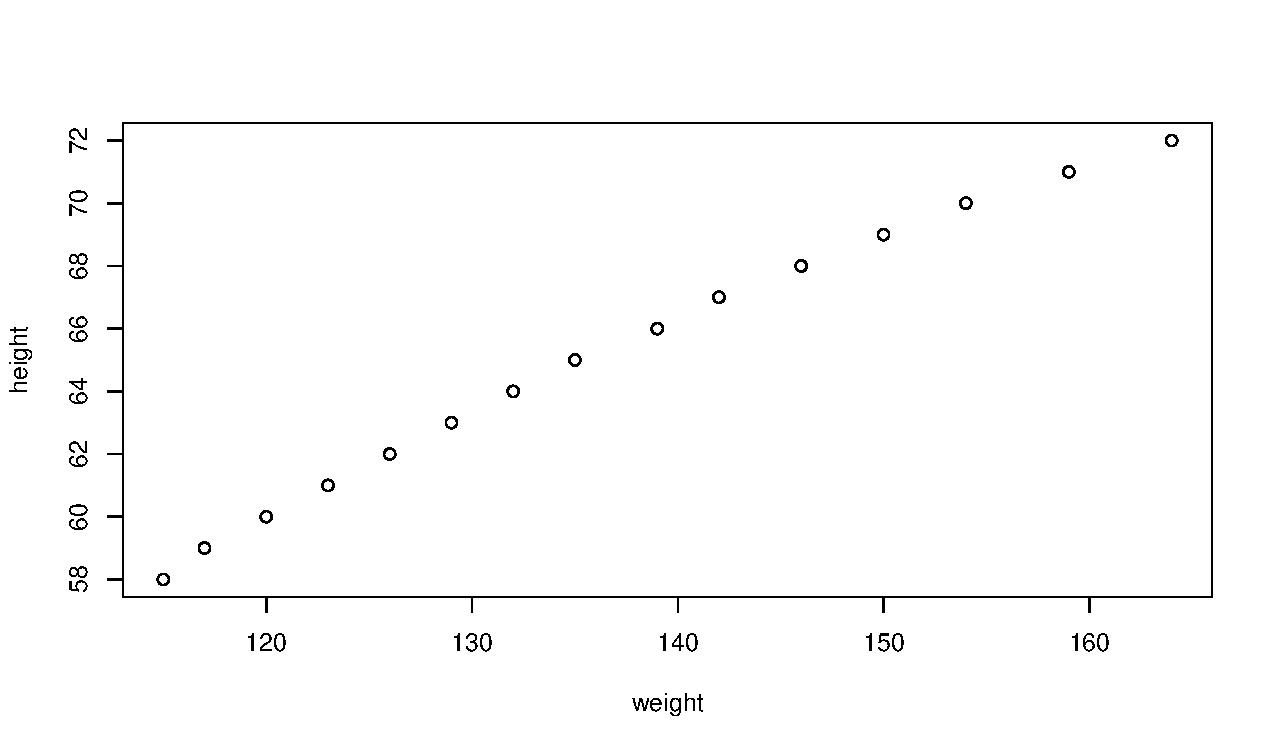
\includegraphics[width=\maxwidth]{figure/unnamed-chunk-45-1} 

}


\end{knitrout}

Thus, we decide to use Ratio Sampling.
\begin{knitrout}
\definecolor{shadecolor}{rgb}{0.969, 0.969, 0.969}\color{fgcolor}\begin{kframe}
\begin{alltt}
\hlstd{Sqrt_weights} \hlkwb{=} \hlkwd{sqrt}\hlstd{(sample_weights)}
\hlstd{sample_weights} \hlkwb{=} \hlstd{sample_weights}\hlopt{/}\hlstd{Sqrt_weights}
\hlstd{sample_heights} \hlkwb{=} \hlstd{sample_heights}\hlopt{/}\hlstd{Sqrt_weights}
\end{alltt}
\end{kframe}
\end{knitrout}
\begin{itemize}
    \item \code{Sqrt\_weights = sqrt(sample\_weights)} $=\sqrt{x_i}$.
    \item \code{sample\_weights = sample\_weights / Sqrt\_weights} $=x_i/\sqrt{x_i}$.
    \item \code{sample\_heights = sample\_heights / Sqrt\_weights} $=y_i/\sqrt{x_i}$.
\end{itemize}
In order to remove the intercept, we need to use the \code{-1} in the following code.
\begin{knitrout}
\definecolor{shadecolor}{rgb}{0.969, 0.969, 0.969}\color{fgcolor}\begin{kframe}
\begin{alltt}
\hlstd{sum} \hlkwb{<-} \hlkwd{summary}\hlstd{(}\hlkwd{lm}\hlstd{(sample_heights} \hlopt{~} \hlstd{sample_weights} \hlopt{-} \hlnum{1}\hlstd{))}
\hlkwd{print}\hlstd{(sum)}
\end{alltt}
\begin{verbatim}
## 
## Call:
## lm(formula = sample_heights ~ sample_weights - 1)
## 
## Residuals:
##        1        2        3        4        5 
##  0.11626  0.03317 -0.04613 -0.23802  0.15937 
## 
## Coefficients:
##                Estimate Std. Error t value Pr(>|t|)    
## sample_weights  0.48545    0.00615   78.93 1.54e-07 ***
## ---
## Signif. codes:  0 '***' 0.001 '**' 0.01 '*' 0.05 '.' 0.1 ' ' 1
## 
## Residual standard error: 0.1572 on 4 degrees of freedom
## Multiple R-squared:  0.9994,	Adjusted R-squared:  0.9992 
## F-statistic:  6231 on 1 and 4 DF,  p-value: 1.544e-07
\end{verbatim}
\end{kframe}
\end{knitrout}
\begin{itemize}
    \item $\hat{\beta}=0.48545$
    \item $\hat{\sigma}_{\text{ratio}}=0.1572$
          $$\hat{\mu}_{\text{height}}=\hat{\beta}x_i=\frac{\bar{y}}{\bar{x}}=\frac{63.4}{130.6}x_i=0.48545x_i$$
          which is our line of best fit.
\end{itemize}

The ratio estimate is
$$\hat{\mu}_{\text{ratio}}=\hat{\mu}_{\text{height}}(\mu_{\text{weight}})=0.48545(136.7333)=66.4$$
Well the real answer, was $65$, so we are $1.4$ units away from the real answer.
However, that was closer than SRS which was $1.6$ units away from the real answer.

\begin{knitrout}
\definecolor{shadecolor}{rgb}{0.969, 0.969, 0.969}\color{fgcolor}\begin{kframe}
\begin{alltt}
\hlstd{beta} \hlkwb{<-} \hlstd{sum}\hlopt{$}\hlstd{coefficients[}\hlnum{1}\hlstd{]}
\hlstd{mu_ratio} \hlkwb{<-} \hlstd{beta} \hlopt{*} \hlstd{mu_weight}
\hlstd{sigma_ratio} \hlkwb{<-} \hlstd{sum}\hlopt{$}\hlstd{sigma}
\hlstd{n} \hlkwb{<-} \hlnum{5}
\hlstd{N} \hlkwb{<-} \hlnum{15}
\hlstd{c} \hlkwb{<-} \hlkwd{qnorm}\hlstd{(}\hlnum{0.975}\hlstd{)}
\hlkwd{round}\hlstd{(mu_ratio} \hlopt{+} \hlkwd{c}\hlstd{(}\hlopt{-}\hlnum{1}\hlstd{,} \hlnum{1}\hlstd{)} \hlopt{*} \hlstd{((c} \hlopt{*} \hlstd{sigma_ratio)}\hlopt{/}\hlkwd{sqrt}\hlstd{(n))} \hlopt{*} \hlkwd{sqrt}\hlstd{(}\hlnum{1} \hlopt{-}
  \hlstd{n}\hlopt{/}\hlstd{N),} \hlnum{1}\hlstd{)}
\end{alltt}
\begin{verbatim}
## [1] 66.3 66.5
\end{verbatim}
\end{kframe}
\end{knitrout}

A 95\% confidence interval for $\mu_y$ is:
$$\hat{\mu}_{\text{ratio}}\pm \frac{c\hat{\sigma}_{\text{ratio}}}{\sqrt{n}}\sqrt{1-\frac{n}{N}}=66.4\pm \frac{1.96(0.1572)}{\sqrt{5}}\sqrt{1-\frac{5}{15}}=(66.3,66.5)$$
Width: $0.2$

Note:
\begin{itemize}
    \item Width of CI using Ratios is narrower than SRS.
    \item There is bias in ratio estimation. Notice that the interval doesn't
          contain 65 which is the real answer.
\end{itemize}

Requirements:
\begin{itemize}
    \item Regression and Ratio require highly correlated $Y_i$ and $x_i$.
    \item Ratio requires an intercept of zero.
    \item Both Regression and Ratio are narrower than SRS, but Regression
          and Ratio are both biased.
\end{itemize}

\begin{table}[!htbp]
    \centering
    \begin{NiceTabular}{|c|c|c|}
        \toprule
        Technique &                               Estimate                               &                                                      CI\\
        \midrule
        SRS    &                            $\hat{\mu}_y$                             &              $\displaystyle\hat{\mu}_y\pm \frac{c\hat{\sigma}_y}{\sqrt{n}}\sqrt{1-\frac{n}{N}}$              \\
        Reg    &     $\hat{\mu}_{\text{reg}}=\bar{y}+\hat{\beta}(\mu_x-\bar{x})$      &   $\displaystyle\hat{\mu}_{\text{reg}}\pm \frac{c\hat{\sigma}_{\text{reg}}}{\sqrt{n}}\sqrt{1-\frac{n}{N}}$   \\
        Ratio   & $\hat{\mu}_{\text{ratio}}=\displaystyle\frac{\bar{y}}{\bar{x}}\mu_x$ & $\displaystyle\hat{\mu}_{\text{ratio}}\pm \frac{c\hat{\sigma}_{\text{ratio}}}{\sqrt{n}}\sqrt{1-\frac{n}{N}}$ \\
        \bottomrule
    \end{NiceTabular}
\end{table}
\section{Lecture 41.00: Ratio Estimation}
Suppose we had six students in our class. We selected them out at random
using SRS\@. We record their grade in Calculus 1 and their gender.
\[ \begin{matrix}
        \text{Gender} & \text{Grade} \\
        \midrule
        M             & 70           \\
        F             & 70           \\
        M             & 85           \\
        F             & 85           \\
        M             & 90           \\
        F             & 90
    \end{matrix} \]
The males on average: $ \bar{x}_M=(70+85+90)/3 $.
Let
\begin{itemize}
    \item $ y_i $ be the grade, and
    \item $ z_i=\begin{cases}
                  1 & \text{ if male}  \\
                  0 & \text{otherwise}
              \end{cases} $
\end{itemize}
Our estimate is $ \hat{\theta} $,
\[ \hat{\theta}=\frac{\sum_{i\in\mathcal{S}}y_i z_i}{\sum_{i\in \mathcal{S}}z_i }  \]
\begin{itemize}
    \item $ \sum_{i\in\mathcal{S}}y_i z_i $ counts the number of grades of those males.
    \item $ \sum_{i\in\mathcal{S}} z_i $ counts the number of males you happen to have.
\end{itemize}
Our parameter is $ \theta $,
\[ \theta=\frac{\sum_{i=1}^{N} \frac{y_i z_i}{N} }{\sum_{i=1}^{N} \frac{z_i}{N} }=\frac{\mu}{\pi}   \]
\begin{itemize}
    \item $ \mu $ is the average of the male grades.
    \item $ \pi $ is the proportion of the people that are male.
\end{itemize}
Therefore, we can write our estimate as $ \hat{\theta}=\hat{\mu}/\hat{\pi} $.
\subsection*{Estimator}
Our estimator asks ``what's random?''
What's random is whether you're in the sample.
We define an indicator variable $ I_i $ which will be 1 if it's in our population.
\[ \tilde{\theta}=\frac{\frac{\sum_{i=1}^{N}I_i y_i z_i}{n} }{\frac{\sum_{i=1}^{N} I_i z_i}{n}}=\frac{\tilde{\mu}}{\tilde{\pi}}   \]
Now there's a bit of math involved in this because unfortunately we have never
looked at the ratio of two random variables, and it's very difficult to do.
Instead, we're going to use \emph{Taylor's Approximation} (Lecture 41.50 goes more in detail).

Taylor's Approximation gives:
\[ \frac{\tilde{\mu}}{\tilde{\pi}}\approx \frac{\mu}{\pi}+\frac{1}{\pi}(\tilde{\mu}-\mu)-\frac{\mu}{\pi^2}(\tilde{\pi}-\pi)  \]
where $ \tilde{\mu} $ and $ \tilde{\pi} $ are both obtained by SRS\@. So we obtain the proportion and average from simple random sampling.
\begin{itemize}
    \item The approximation is approximately normal (there's a Gaussian extension that allows
          this to be true).
\end{itemize}
\subsection*{Expectation and Variance}
\begin{align*}
    \E*{\frac{\tilde{\mu}}{\tilde{\pi}}}
     & \approx \E*{\frac{\mu}{\pi}+\frac{1}{\pi}(\tilde{\mu}-\mu)-\frac{\mu}{\pi^2}(\tilde{\pi}-\pi)}                         \\
     & =\frac{\mu}{\pi}+\frac{1}{\pi} \biggl(\E*{\tilde{\mu}}-\mu\biggr)-\frac{\mu}{\pi^2} \biggl(\E*{\tilde{\pi}}-\pi\biggr) \\
     & =\frac{\mu}{\pi}
\end{align*}
since $ \E{\tilde{\mu}}=\mu $ and $ \E*{\tilde{\pi}}=\pi $ (by SRS, unbiased).
\begin{align*}
    \Var*{\frac{\tilde{\mu}}{\tilde{\pi}}}
     & \approx \Var*{\frac{\mu}{\pi}+\frac{1}{\pi}(\tilde{\mu}-\mu)-\frac{\mu}{\pi^2}(\tilde{\pi}-\pi)} \\
     & =\frac{1}{\pi^2} \Var{\tilde{\mu}-\mu-\frac{\mu\tilde{\pi}}{\pi}+\mu}                            \\
     & =\frac{1}{\pi^2} \Var*{\tilde{\mu}-\frac{\mu \tilde{\pi}}{\pi}}
\end{align*}
This is an average. Therefore, we end up with an estimated variance.
\[  \Var*{\frac{\tilde{\mu}}{\tilde{\pi}}}\approx \frac{1}{\pi^2} \frac{\sigma^2_{\text{ratio}}}{n}\biggl(1-\frac{n}{N}\biggr)  \]
A confidence interval is:
\[ \text{EST}\pm c\,\text{SE}=\hat{\theta}\pm c\, \frac{1}{\hat{\pi}} \sqrt{1-\frac{n}{N}}\frac{\hat{\sigma}_{\text{ratio}}}{\sqrt{n}}  \]
where
\[ \hat{\sigma}_{\text{ratio}}^2=\frac{\sum_{i\in\mathcal{S}}\bigl(y_i-\hat{\theta}z_i\bigr)^2 }{n-1}  \]
\section{Lecture 41.50: Taylor's Approximation}
\emph{Calculus 1}: $ f(x)\approx f(x_0)+f^\prime(x_0)(x-x_0) $.
\begin{Example}{Calculus 1 Taylor's Approximation}{}
    Approximate $ f(1.1)=\ln(1.1) $ about $ x_0=1 $.

    \textbf{Solution.}
    \[ f(1.1)\approx f(1)+f^\prime(1)(1.1-1)=\ln(1)+\frac{1}{x}\bigg\vert_{x=1} (1.1-1)=0+1(0.1)=0.1 \]
\end{Example}
\emph{Calculus 3}:
\[ f(x,y)\approx f(x_0,y_0)+\pdv{f(x_0,y_0)}{x}(x-x_0)+\pdv{f(x_0,y_0)}{y}(y-y_0) \]
\begin{Example}{Calculus 3 Taylor's Approximation}{}
    Approximate $ f(1.1,1.1)=\ln(1.1\times 1.1) $ about the point $ (1,1) $.

    \textbf{Solution.}
    \begin{align*}
        f(1.1,1.1)
         & \approx f(1,1)+\pdv{f(1,1)}{x}(x-x_0)+\pdv{f(1,1)}{y}(y-y_0)                          \\
         & =\ln(1)+\frac{1}{x}\bigg\vert_{x=1,y=1}(1.1-1)+\frac{1}{y}\bigg\vert_{x=1,y=1}(1.1-1) \\
         & =0+0.1+0.1                                                                            \\
         & =0.2
    \end{align*}
\end{Example}
Approximate: $ f(x,y)=x/y $ about the point $ (x_0,y_0) $.
\begin{align*}
    f(x,y)
     & \approx f(x_0,y_0)+\frac{1}{y_0}(x-x_0)+\biggl(-\frac{x_0}{y_0^2} \biggr)(y-y_0) \\
     & =\frac{x_0}{y_0}+\frac{1}{y_0} (x-x_0)-\frac{x_0}{y_0^2}(y-y_0)
\end{align*}
Therefore, approximating $ \tilde{\mu}/\tilde{\pi} $ about $ (\mu,\pi) $:
\[ \frac{\tilde{\mu}}{\tilde{\pi}}\approx \frac{\mu}{\pi}+\frac{1}{\pi} (\tilde{\mu}-\mu)-\frac{\mu}{\pi^2}(\tilde{\pi}-\pi)   \]

\section{Lecture 42.00: Ratio Estimation, Example}
\begin{Example}{}{}
    The number of people in the Kitchener riding is
    $89\,422$. Stephen Harper wants to know the average age
    of people in the riding who would vote for him. Using SRSWOR,
    he selects $80$ people, and finds that the average age of those
    who vote for him is $67$. $42$ of those poled would vote for him.
    If the estimated variance is $5.42$, build a $95\%$ confidence interval
    for the average age of those who vote for Stephen Harper.

    \textbf{Solution.}
    \begin{itemize}
        \item The proportion of people that
              would vote for Stephen Harper is $ \hat{\pi}=42/80 $.
        \item The average age of those that would vote for him is
              $ \hat{\theta}=\hat{\mu}/\hat{\pi}=67 $.
    \end{itemize}
    Therefore, a $95\%$ confidence interval for the average age of those who
    vote for Stephen Harper is:
    \begin{align*}
        \hat{\theta}\pm c\, \frac{1}{\hat{\pi}} \frac{\hat{\sigma}_{\text{ratio}}}{\sqrt{n}}\sqrt{1-\frac{n}{N}}
         & =67\pm 1.96\biggl(\frac{1}{42/80}\biggr) \sqrt{\frac{5.42}{80}} \sqrt{1-\frac{80}{89422}} \\
         & =(66.03,67.97)
    \end{align*}
\end{Example}


\chapter{Assignment 9}
\section{Lecture 43.00: Stratified Sampling}
Suppose that you're interested in the population as a whole,
but at the same time you're interested in some sub-population of the population.
For example suppose you're interested in University of Waterloo students,
but we're also interested in Math faculty students.
You would use a \emph{stratified} sample.
In this case, you might perform SRS over a sub-population and then
combine that together to get the entire population so what would that notationally
look like?

Suppose we have a frame $ U $, and we divide $ U $ into sub-frames
$ U_1,U_2,\ldots,U_H $ where
\begin{enumerate}[(1)]
    \item $ U_1\cup U_2\cup U_3\cup \cdots \cup U_H=U $.
    \item For any $ i\ne j $, $ U_i\cap U_j=\emptyset $.
    \item Define $ \abs{U_h}=N_h $ and $ \abs{U}=N $.
    \item $ N_1+N_2+\cdots+N_h=N $.
\end{enumerate}
\subsubsection*{Parameter}
\begin{align*}
    \mu
     & =\frac{N_1 \mu_1+N_2 \mu_2+\cdots+N_H \mu_H}{N}                     \\
     & =\frac{N_1}{N} \mu_1+\frac{N_2}{N} \mu_2+\cdots+\frac{N_h}{N} \mu_H \\
     & =w_1 \mu_1+\cdots+w_H \mu_H                                         \\
     & =\sum_{i=1}^{H} w_i \mu_i
\end{align*}
\subsubsection*{Estimate}
We would use SRS to estimate the strata's average.
\[ \hat{\mu}=\sum_{i=1}^{H} w_i\hat{\mu}_i \]
When we get the strata's average,
and we multiply by the weight we add over the strata's to
get the population average.
\subsubsection*{Estimator}
\[ \tilde{\mu}=\sum_{i=1}^{H} w_i\tilde{\mu}_i \]
where $ \tilde{\mu}_i $ is the SRS random variable, hence it is unbiased
and normally distributed. Therefore, the weighted average of the estimator
will be normally distributed. Now, we need to find the expectation and variance
of $ \tilde{\mu} $.
\subsubsection*{Expectation of $ \tilde{\mu} $}
\[ \E*{\tilde{\mu}}=\E*{\sum_{i=1}^{H} w_i\tilde{\mu}_i}=\sum_{i=1}^{H} w_i\E{\tilde{\mu}_i}=
    \sum_{i=1}^{H} w_i \mu_i\quad\text{since SRS is unbiased.} \]
\subsubsection*{Variance of $ \tilde{\mu} $}
At this point in the course the formulas become ugly.
\[ \Var*{\tilde{\mu}}=\Var*{\sum_{i=1}^{H} w_i\tilde{\mu}_i}=\sum_{i=1}^{H} w_i^2\Var*{\tilde{\mu}_i} \]
where $ \tilde{\mu}_i\indep \tilde{\mu}_j $ since no unit is in both groups. Therefore,
\[ \Var*{\tilde{\mu}}=\sum_{i=1}^{H}w_i^2 \frac{\sigma_i^2}{n_i} \biggl(1-\frac{n_i}{N_i} \biggr) \]
\subsubsection*{Confidence Interval for $ \mu $}
\[ \hat{\mu}\pm c\sqrt{\sum_{i=1}^{H}w_i^2 \frac{\sigma_i^2}{n_i} \biggl(1-\frac{n_i}{N_i} \biggr)}\quad\text{where $ c \sim \N{0,1} $.} \]
\subsection*{Proportion}
For a proportion, we want to estimate $ \pi $.
\subsubsection*{Parameter}
\[ \pi=\sum_{i=1}^{H} w_i \pi_i \]
\subsubsection*{Estimate}
\[ \hat{\pi}=\sum_{i=1}^{H} w_i\hat{\pi}_i\quad\text{which uses SRS.} \]
\subsubsection*{Estimator}
\[ \tilde{\pi}=\sum_{i=1}^{H} w_i\tilde{\pi}_i \]
\subsubsection*{Confidence Interval for $ \pi $}
\[ \hat{\pi}\pm c\sqrt{\sum_{i=1}^{H}w_i^2 \frac{\sigma_i^2}{n_i} \biggl(1-\frac{n_i}{N_i} \biggr)}\quad\text{where $ c \sim \N{0,1} $.} \]
You'll remember that we have worked out before that $ \sigma_i^2=\pi_i(1-\pi_i) $.

\section{Lecture 44.00: Stratified, Allocation}
Today we're going to talk about something called \emph{Allocation}.
For example, allocation is when you have a sample of $100$ units,
and you have four strata. How should you spend those $100$ units?
Should three quarters of them go to one stratum, and the remaining quarter be split
among the last three strata? We define how you divide them up to be stratification.
To make that decision there are two types that we're going to talk about today.
\begin{enumerate}[(1)]
    \item Proportional.
    \item Neyman or optimal.
\end{enumerate}
\subsection*{Proportional}
We sample based on the size of the strata. In other words, the bigger
the strata size, the bigger the sample size.
\[ n_h=w_h n \]
\begin{Example}{}{}
    \[ \begin{matrix}
            \text{Provinces} & \text{Population (millions)} \\
            \midrule
            \text{ON}        & 10                           \\
            \text{QUE}       & 5                            \\
            \text{BC}        & 3                            \\
            \text{ALB}       & 2                            \\
            \midrule
            \text{Total}     & 20
        \end{matrix} \]
    If we have $ n=100 $ units to sample, ON should get $ n_{\text{ON}}=w_{\text{ON}}(n)=1/2(100)=50 $
    units.
\end{Example}
\subsection*{Neyman}
In Neyman allocation, we select our sample size and values that minimize the stratified variance.
\[ \Var{\tilde{\mu}}=\sum_{i=1}^{H} w_i^2 \frac{\sigma_i^2}{n_i} \biggl(1-\frac{n_i}{N_i} \biggr) \]
subject to $ n=n_1+n_2+\cdots+n_H $. This ends up being a Lagrange multiplication problem.
So minimize
\[ W(\tilde{\mu})=\sum_{i=1}^{H} w_i^2 \frac{\sigma_i^2}{n_i} \biggl(1-\frac{n_i}{N_i} \biggr)+
    \lambda(n-n_1-\cdots-n_H) \]
Find $ \pd{W}{\lambda},\pd{W}{n_i} $ and set to zero to get:
\[ n_i=\frac{n\sigma_i w_i}{\sum_{j=1}^{H} \sigma_j w_j}  \]
\begin{Remark}{}{}
    \begin{itemize}
        \item $ n_i \propto \sigma_i $. So, if you have more variability in your stratum,
              then you're going to want a larger sample size. That should make a lot of
              sense because if you have a lot of variability, you can reduce the variability
              by having a larger sample size, remember, the variability
              is the average of the variance divided by $ n $.
              So, the larger your sample size the smaller the variance ends up being.
        \item $ n_i\propto w_i $. The larger the strata, the more
              units you will want allocated to it.
        \item If $ \sigma_1=\sigma_2=\cdots=\sigma_H $, then
              \[ n_i=\frac{n w_i}{\sum_{i=1}^{H} w_i}=n w_i  \]
              which is proportional allocation since $ \sum_{i=1}^{H} w_i=1 $.
    \end{itemize}
\end{Remark}
Just like when we did with the small sample size, we take a small sample, and you use the small sample
to estimate these unknown $ \sigma $'s. Once you've estimated these unknown $ \sigma $'s,
you'd use them to determine how you should allocate your larger sample size to the actual strata of interest.


\section{Lecture 45.00: Stratified Example}
\subsection{Stratified 1}\label{stratified1}
I am interested in the average tuition paid by students
at the University of Waterloo. Additionally, I want
to know how much each faculty student is paying on average.
Hence, I decide to stratify by Faculty (assume students belong to a single faculty).
\begin{table}[!htbp]
    \centering
    \begin{NiceTabular}{|c|c|c|c|c|c|}
        \toprule
        Faculty & $ N $ & $ \hat{\mu} $ & $ n $ & $ W $ & $ \hat{\sigma} $\\
        \midrule
        Math   & 6600  &    4500     &  15   & 0.22  &      400       \\
        Arts   & 9000  &    3000     &  10   & 0.30  &      200       \\
        Science  & 5400  &    4500     &  25   & 0.18  &      300       \\
        AHS    & 1500  &    3200     &  35   & 0.05  &      100       \\
        Engineer & 6000  &    7000     &  15   & 0.20  &      100       \\
        EVS    & 1500  &    3500     &  20   & 0.05  &      200       \\
        Total   & 30000 &             &  120  \\
        \bottomrule
    \end{NiceTabular}
\end{table}
\subsubsection*{Build a 95\% confidence interval for the mean tuition in Math.}
\begin{knitrout}
\definecolor{shadecolor}{rgb}{0.969, 0.969, 0.969}\color{fgcolor}\begin{kframe}
\begin{alltt}
\hlstd{ci} \hlkwb{<-} \hlnum{4500} \hlopt{+} \hlkwd{c}\hlstd{(}\hlopt{-}\hlnum{1}\hlstd{,} \hlnum{1}\hlstd{)} \hlopt{*} \hlkwd{qnorm}\hlstd{(}\hlnum{0.975}\hlstd{)} \hlopt{*} \hlnum{400}\hlopt{/}\hlkwd{sqrt}\hlstd{(}\hlnum{15}\hlstd{)} \hlopt{*} \hlstd{(}\hlnum{1} \hlopt{-} \hlnum{15}\hlopt{/}\hlnum{6600}\hlstd{)}
\hlkwd{round}\hlstd{(ci)}
\end{alltt}
\begin{verbatim}
## [1] 4298 4702
\end{verbatim}
\end{kframe}
\end{knitrout}
\[ \hat{\mu}_\text{math}\pm\frac{c\hat{\sigma}_\text{math}}{\sqrt{n_\text{math}}}\sqrt{1-\frac{n_\text{math}}{N_\text{math}}}=4500\pm \frac{1.96(400)}{\sqrt{15}} \sqrt{1-\frac{15}{6600} }=(4298,4702)\]
\subsubsection*{Build a 95\% confidence interval for the mean tuition at UW.}
Since we've used SRS in each of the strata, we have to use stratified sampling.
\begin{knitrout}
\definecolor{shadecolor}{rgb}{0.969, 0.969, 0.969}\color{fgcolor}\begin{kframe}
\begin{alltt}
\hlstd{N_i} \hlkwb{<-} \hlkwd{c}\hlstd{(}\hlnum{6600}\hlstd{,} \hlnum{9000}\hlstd{,} \hlnum{5400}\hlstd{,} \hlnum{1500}\hlstd{,} \hlnum{6000}\hlstd{,} \hlnum{1500}\hlstd{)}
\hlstd{N} \hlkwb{<-} \hlkwd{sum}\hlstd{(N_i)}
\hlstd{w_i} \hlkwb{<-} \hlstd{N_i}\hlopt{/}\hlstd{N}
\hlstd{n_i} \hlkwb{<-} \hlkwd{c}\hlstd{(}\hlnum{15}\hlstd{,} \hlnum{10}\hlstd{,} \hlnum{25}\hlstd{,} \hlnum{35}\hlstd{,} \hlnum{15}\hlstd{,} \hlnum{20}\hlstd{)}
\hlstd{mu_i} \hlkwb{<-} \hlkwd{c}\hlstd{(}\hlnum{4500}\hlstd{,} \hlnum{3000}\hlstd{,} \hlnum{4500}\hlstd{,} \hlnum{3200}\hlstd{,} \hlnum{7000}\hlstd{,} \hlnum{3500}\hlstd{)}
\hlstd{sigma_i} \hlkwb{<-} \hlkwd{c}\hlstd{(}\hlnum{400}\hlstd{,} \hlnum{200}\hlstd{,} \hlnum{300}\hlstd{,} \hlnum{100}\hlstd{,} \hlnum{100}\hlstd{,} \hlnum{200}\hlstd{)}
\hlstd{mu} \hlkwb{<-} \hlkwd{sum}\hlstd{(w_i} \hlopt{*} \hlstd{mu_i)}
\hlstd{variance} \hlkwb{<-} \hlkwd{sum}\hlstd{(w_i}\hlopt{^}\hlnum{2} \hlopt{*} \hlstd{sigma_i}\hlopt{^}\hlnum{2}\hlopt{/}\hlstd{n_i} \hlopt{*} \hlstd{(}\hlnum{1} \hlopt{-} \hlstd{n_i}\hlopt{/}\hlstd{N_i))}
\hlstd{ci} \hlkwb{<-} \hlstd{mu} \hlopt{+} \hlkwd{c}\hlstd{(}\hlopt{-}\hlnum{1}\hlstd{,} \hlnum{1}\hlstd{)} \hlopt{*} \hlkwd{qnorm}\hlstd{(}\hlnum{0.975}\hlstd{)} \hlopt{*} \hlkwd{sqrt}\hlstd{(variance)}
\hlstd{mu}
\end{alltt}
\begin{verbatim}
## [1] 4435
\end{verbatim}
\begin{alltt}
\hlkwd{round}\hlstd{(variance,} \hlnum{3}\hlstd{)}
\end{alltt}
\begin{verbatim}
## [1] 1023.024
\end{verbatim}
\begin{alltt}
\hlkwd{round}\hlstd{(ci)}
\end{alltt}
\begin{verbatim}
## [1] 4372 4498
\end{verbatim}
\end{kframe}
\end{knitrout}
\[ \hat{\mu}=\sum_{i=1}^H w_i \hat{\mu}_i=4435 \]
\[ \widehat{\mathbb{V}(\tilde{\mu})}=\sum_{i=1}^{H} \frac{w_i^2\hat{\sigma}_i^2}{n_i}\biggl(1-\frac{n_i}{N_i} \biggr)=1023.024 \]
Therefore, a 95\% confidence interval for $\mu$ is:
\[ \hat{\mu}\pm c\sqrt{\widehat{\mathbb{V}(\tilde{\mu})}}=4435\pm 1.96\sqrt{1023.024}=(4372, 4498) \]
\subsection{Stratified 2}
We continue from~\Cref{stratified1}.
\subsubsection*{A proportional allocation of our sample values to each stratum.}
\begin{knitrout}
\definecolor{shadecolor}{rgb}{0.969, 0.969, 0.969}\color{fgcolor}\begin{kframe}
\begin{alltt}
\hlstd{n} \hlkwb{<-} \hlnum{120}
\hlkwd{round}\hlstd{(n} \hlopt{*} \hlstd{w_i)}
\end{alltt}
\begin{verbatim}
## [1] 26 36 22  6 24  6
\end{verbatim}
\end{kframe}
\end{knitrout}
\begin{itemize}
    \item $n_\text{math}=n w_\text{math}=120(0.22)=26$.
    \item $n_\text{arts}=36$.
    \item $n_\text{science}=22$.
    \item $n_{\text{ahs}}=6$.
    \item $n_{\text{eng}}=24$.
    \item $n_{\text{evs}}=6$.
\end{itemize}

\subsubsection*{An optimal allocation of our sample values to each stratum.}
\begin{knitrout}
\definecolor{shadecolor}{rgb}{0.969, 0.969, 0.969}\color{fgcolor}\begin{kframe}
\begin{alltt}
\hlkwd{round}\hlstd{(n} \hlopt{*} \hlstd{sigma_i} \hlopt{*} \hlstd{w_i}\hlopt{/}\hlkwd{sum}\hlstd{(w_i} \hlopt{*} \hlstd{sigma_i))}
\end{alltt}
\begin{verbatim}
## [1] 45 30 27  3 10  5
\end{verbatim}
\end{kframe}
\end{knitrout}
\begin{itemize}
    \item $n_\text{math}=\dfrac{n\sigma_\text{math}w_\text{math}}{\sum_{j=1}^{6} w_j \sigma_j}=\frac{120(400)(0.22)}{237}=45$.
    \item $n_\text{arts}=30$.
    \item $n_\text{science}=27$.
    \item $n_{\text{ahs}}=3$.
    \item $n_{\text{eng}}=10$.
    \item $n_{\text{evs}}=120-45-30-27-3-10=5$.
\end{itemize}

\subsection{Stratified 3}
A course has 3 sections all taught by one instructor. There
are $205$, $212$, and $253$ people in each of the sections
$1$, $2$, and $3$ respectively. At the end of the term the instructor
is curious about how well the students performed. The administration
takes a simple random sampling of $15$, $12$, and $14$ people respectively from each section.
The averages for each section are $75$, $70$, and $72$ respectively
with standard deviations of $10$, $15$, and $5$. Build a 95%
confidence interval for the mean grade of the instructors course.

\begin{knitrout}
\definecolor{shadecolor}{rgb}{0.969, 0.969, 0.969}\color{fgcolor}\begin{kframe}
\begin{alltt}
\hlstd{N_i} \hlkwb{<-} \hlkwd{c}\hlstd{(}\hlnum{205}\hlstd{,} \hlnum{212}\hlstd{,} \hlnum{253}\hlstd{)}
\hlstd{N} \hlkwb{<-} \hlkwd{sum}\hlstd{(N_i)}
\hlstd{w_i} \hlkwb{<-} \hlstd{N_i}\hlopt{/}\hlstd{N}
\hlstd{n_i} \hlkwb{<-} \hlkwd{c}\hlstd{(}\hlnum{15}\hlstd{,} \hlnum{12}\hlstd{,} \hlnum{14}\hlstd{)}
\hlstd{mu_i} \hlkwb{<-} \hlkwd{c}\hlstd{(}\hlnum{75}\hlstd{,} \hlnum{70}\hlstd{,} \hlnum{72}\hlstd{)}
\hlstd{sigma_i} \hlkwb{<-} \hlkwd{c}\hlstd{(}\hlnum{10}\hlstd{,} \hlnum{15}\hlstd{,} \hlnum{5}\hlstd{)}
\hlstd{mu} \hlkwb{<-} \hlkwd{sum}\hlstd{(w_i} \hlopt{*} \hlstd{mu_i)}
\hlstd{variance} \hlkwb{<-} \hlkwd{sum}\hlstd{(w_i}\hlopt{^}\hlnum{2} \hlopt{*} \hlstd{sigma_i}\hlopt{^}\hlnum{2}\hlopt{/}\hlstd{n_i} \hlopt{*} \hlstd{(}\hlnum{1} \hlopt{-} \hlstd{n_i}\hlopt{/}\hlstd{N_i))}
\hlstd{ci} \hlkwb{<-} \hlstd{mu} \hlopt{+} \hlkwd{c}\hlstd{(}\hlopt{-}\hlnum{1}\hlstd{,} \hlnum{1}\hlstd{)} \hlopt{*} \hlkwd{qnorm}\hlstd{(}\hlnum{0.975}\hlstd{)} \hlopt{*} \hlkwd{sqrt}\hlstd{(variance)}
\hlstd{mu}
\end{alltt}
\begin{verbatim}
## [1] 72.28507
\end{verbatim}
\begin{alltt}
\hlstd{variance}
\end{alltt}
\begin{verbatim}
## [1] 2.589983
\end{verbatim}
\begin{alltt}
\hlkwd{round}\hlstd{(ci,} \hlnum{3}\hlstd{)}
\end{alltt}
\begin{verbatim}
## [1] 69.131 75.439
\end{verbatim}
\end{kframe}
\end{knitrout}

\[ \hat{\mu}=\sum_{i=1}^H w_i \hat{\mu}_i=72.28507 \]
\[\widehat{\mathbb{V}(\tilde{\mu})}=\sum_{i=1}^{H} \frac{w_i^2\hat{\sigma}_i^2}{n_i}\biggl(1-\frac{n_i}{N_i} \biggr)=2.589983 \]
Therefore, a 95\% confidence interval for $\mu$ is:
\[\hat{\mu}\pm c\sqrt{\widehat{\mathbb{V}(\tilde{\mu})}}=72.28507\pm 1.96\sqrt{2.589983}=(69.131,75.439) \]
\section{Lecture 46.00: Post Stratification}
Until now what you had some strata, performed SRS on each stratum, then
combined them, and looked at the population value $ \mu $. See~\Cref{fig:strata}.
\begin{figure}[!htbp]
    \centering
    \begin{tikzpicture}[x=0.75pt,y=0.75pt,yscale=-1,xscale=1]
        %uncomment if require: \path (0,162); %set diagram left start at 0, and has height of 162

        %Shape: Rectangle [id:dp6861764355714591] 
        \draw   (12,9) -- (82,9) -- (82,49) -- (12,49) -- cycle ;
        %Shape: Rectangle [id:dp7925417207393711] 
        \draw   (12,60) -- (82,60) -- (82,100) -- (12,100) -- cycle ;
        %Shape: Rectangle [id:dp9116080179254983] 
        \draw   (12,111) -- (82,111) -- (82,151) -- (12,151) -- cycle ;
        %Straight Lines [id:da42452853568114324] 
        \draw    (83,27) -- (163.33,79.9) ;
        \draw [shift={(165,81)}, rotate = 213.37] [color={rgb, 255:red, 0; green, 0; blue, 0 }  ][line width=0.75]    (10.93,-3.29) .. controls (6.95,-1.4) and (3.31,-0.3) .. (0,0) .. controls (3.31,0.3) and (6.95,1.4) .. (10.93,3.29)   ;
        %Straight Lines [id:da2851258632117559] 
        \draw    (84,81) -- (163,81) ;
        \draw [shift={(165,81)}, rotate = 180] [color={rgb, 255:red, 0; green, 0; blue, 0 }  ][line width=0.75]    (10.93,-3.29) .. controls (6.95,-1.4) and (3.31,-0.3) .. (0,0) .. controls (3.31,0.3) and (6.95,1.4) .. (10.93,3.29)   ;
        %Straight Lines [id:da06580588611951421] 
        \draw    (84,130) -- (163.29,82.04) ;
        \draw [shift={(165,81)}, rotate = 508.83] [color={rgb, 255:red, 0; green, 0; blue, 0 }  ][line width=0.75]    (10.93,-3.29) .. controls (6.95,-1.4) and (3.31,-0.3) .. (0,0) .. controls (3.31,0.3) and (6.95,1.4) .. (10.93,3.29)   ;
        %Shape: Rectangle [id:dp33582592326822736] 
        \draw   (161,40) -- (201,40) -- (201,119) -- (161,119) -- cycle ;
        %Straight Lines [id:da11175824112302257] 
        \draw    (162,66) -- (201,66) ;
        %Straight Lines [id:da37350978775751853] 
        \draw    (162,96) -- (201,96) ;

        % Text Node
        \draw (203,80.2) node [anchor=west] [inner sep=0.75pt]    {$\mu $};
        % Text Node
        \draw (47,29) node   [align=left] {SRS};
        % Text Node
        \draw (47,80) node   [align=left] {SRS};
        % Text Node
        \draw (47,131) node   [align=left] {SRS};
    \end{tikzpicture}
    \caption{Regular Stratification}\label{fig:strata}
\end{figure}
In post stratification, the idea is that you have done an SRS
of some large population, and then decided afterwards that you wanted to stratify.
At this point, you then break it into three.
Notice that the SRS is done at the \emph{start} as opposed to at the \emph{end}.
See~\Cref{fig:post_strata}.
\begin{figure}[H]
    \centering
    \begin{tikzpicture}[x=0.75pt,y=0.75pt,yscale=-1,xscale=1]
        %Shape: Rectangle [id:dp9116080179254983] 
        \draw   (12,11) -- (82,11) -- (82,151) -- (12,151) -- cycle ;
        %Straight Lines [id:da42452853568114324] 
        \draw    (83,27) -- (156.5,27) ;
        \draw [shift={(158.5,27)}, rotate = 180] [color={rgb, 255:red, 0; green, 0; blue, 0 }  ][line width=0.75]    (10.93,-3.29) .. controls (6.95,-1.4) and (3.31,-0.3) .. (0,0) .. controls (3.31,0.3) and (6.95,1.4) .. (10.93,3.29)   ;
        %Straight Lines [id:da2851258632117559] 
        \draw    (84,81) -- (156.5,81) ;
        \draw [shift={(158.5,81)}, rotate = 180] [color={rgb, 255:red, 0; green, 0; blue, 0 }  ][line width=0.75]    (10.93,-3.29) .. controls (6.95,-1.4) and (3.31,-0.3) .. (0,0) .. controls (3.31,0.3) and (6.95,1.4) .. (10.93,3.29)   ;
        %Straight Lines [id:da06580588611951421] 
        \draw    (84,130) -- (155.5,129.03) ;
        \draw [shift={(157.5,129)}, rotate = 539.22] [color={rgb, 255:red, 0; green, 0; blue, 0 }  ][line width=0.75]    (10.93,-3.29) .. controls (6.95,-1.4) and (3.31,-0.3) .. (0,0) .. controls (3.31,0.3) and (6.95,1.4) .. (10.93,3.29)   ;
        %Shape: Rectangle [id:dp39278086756839947] 
        \draw   (157.5,115) -- (212,115) -- (212,149) -- (157.5,149) -- cycle ;
        %Shape: Rectangle [id:dp5029651538179899] 
        \draw   (157.5,62.67) -- (212,62.67) -- (212,96.67) -- (157.5,96.67) -- cycle ;
        %Shape: Rectangle [id:dp3267534023424148] 
        \draw   (157.5,10.67) -- (212,10.67) -- (212,44.67) -- (157.5,44.67) -- cycle ;
        % Text Node
        \draw (47,81) node   [align=left] {SRS};
    \end{tikzpicture}
    \caption{Post Stratification}\label{fig:post_strata}
\end{figure}
Mathematically, your sample sizes end up being random, which has an influence on how
we calculate things. Although, it doesn't actually have an influence
on the actual mathematics at the end of the day, so the resultants are the same.
For example, the post stratification estimate is very similar to that of stratified:
\[ \hat{\mu}_{\text{post}}=w_1\mu_1+\cdots+w_H\mu_H \]
The estimated variance for post stratification is:
\[ \widehat{\Var*{\tilde{\mu}_{\text{post}}}}=\sum_{i=1}^{H} w_i^2\biggl(1-\frac{n_i}{N_i}\biggr)\frac{\hat{\sigma}_i^2}{n_i}  \]
A confidence interval for $ \mu_{\text{post}} $ is given by:
\[ \hat{\mu}_{\text{post}}\pm c\sqrt{\widehat{\Var*{\tilde{\mu}_{\text{post}}}}}\quad\text{where $ c \sim \N{0,1} $} \]

\section{Lecture 47.00: Non-Response}
Non-response
means that someone didn't
respond to our survey. All the surveys
of human respondents have non-response.
Non-response causes bias, it is a form of
error that can skew our results. The response
rate (or the proportion of people that respond)
is hard to define and your text goes to some
length to define it. To correct non-response,
we can do something called \emph{two-phase sampling}:
\begin{itemize}
    \item \underline{Phase 1}: Typical SRS with sample size $ n $.
    \item \underline{Phase 2}: Sub-sample $ m $ non-responders from Phase 1.
\end{itemize}
This is a stratified design with responders and non-responders as your strata.

The estimate is
\[ \hat{\mu}=\frac{n_R}{n} \hat{\mu}_R+\frac{n_m}{n} \hat{\mu}_m \]
\begin{itemize}
    \item $ \hat{\mu} = $ population estimate.
    \item $ n_R = $ number of responders.
    \item $ n= $ number of people you ask in general.
    \item $ \hat{\mu}_R= $ response average.
    \item $ n_m= $ number of missing people.
    \item $ \hat{\mu}_m= $ average of the missing people (the non-responders).
\end{itemize}
There's a similar one for the proportion.
\[ \hat{\pi}=\frac{n_R}{n} \hat{\pi}_R+\frac{n_m}{n} \hat{\pi}_m \]
Those are the estimates that you would use.
The variance is very ugly, so we'll ignore it today.


\chapter{Appendix}
Normal:
\[ f(x)=\Prob{X=x}=\frac{1}{\sqrt{2\pi}\sigma}
      \expon*{-\frac{(x-\mu)^2}{2\sigma^2}}  \]
\begin{itemize}
      \item $ F(x)=\Prob{X\le x} $ can be obtained with
            \code{pnorm($x$,$\mu$,$\sigma$)} and gives
            the value of $ p $.
      \item $ F^{-1}(p) $ can be obtained with
            \code{qnorm($p$,$\mu$,$\sigma$)} and gives
            the value of $ x $.
      \item $ f(x)=\Prob{X=x} $ can be obtained with
            \code{dnorm($x$,$\mu$,$\sigma$)}. Note that this is
            \underline{not} a probability.
\end{itemize}
\newpage
\section{Tables}
\subsection*{$ \mathcal{N}(0,1) $ Cumulative Distribution Function}
\pgfmathdeclarefunction{gauss}{2}{%
      \pgfmathparse{1/(#2*sqrt(2*pi))*exp(-((x-#1)^2)/(2*#2^2))}%
}
\begin{table}[!htbp]
      \centering
      \scalebox{0.6}{
            \begin{tikzpicture}
                  \begin{axis}[every axis plot post/.append style={
                                          mark=nonesamples=10000,
                                          smooth},
                              ylabel = $f(x)$,
                              x post scale=1.4
                        ]
                        ]
                        \addplot[draw=none, fill=yellow!50, domain=-3.5:1.2] {gauss(0,1)} \closedcycle;
                        \addplot[very thick,blue!80!black, domain=-3.5:3.5] {gauss(0,1)};
                        \draw[very thick, blue!80!black]  (axis cs:1.2,0) -- (axis cs:1.2, 0.194);
                        \node[below] at (axis cs:1.2,0)  {$x$};
                  \end{axis}
                  \node[below] at (4.5,2)  {$F(x)=\Prob{X\le x}$};
            \end{tikzpicture}}%
      \caption{$ F(x)=\Prob{X\le x} $ where $ X \sim \N{0,1} $} and $ x\ge 0 $
      \begin{tabularx}{\linewidth}{@{}YYZYZYZYZYZY@{}}
            \toprule
            $x$ & 0      & 0.01   & 0.02   & 0.03   & 0.04   & 0.05   & 0.06   & 0.07   & 0.08   & 0.09   \\
            \midrule
            \rowcolor{light-gray}
            0   & 0.5000 & 0.5040 & 0.5080 & 0.5120 & 0.5160 & 0.5199 & 0.5239 & 0.5279 & 0.5319 & 0.5359 \\
            0.1 & 0.5398 & 0.5438 & 0.5478 & 0.5517 & 0.5557 & 0.5596 & 0.5636 & 0.5675 & 0.5714 & 0.5753 \\
            0.2 & 0.5793 & 0.5832 & 0.5871 & 0.5910 & 0.5948 & 0.5987 & 0.6026 & 0.6064 & 0.6103 & 0.6141 \\
            0.3 & 0.6179 & 0.6217 & 0.6255 & 0.6293 & 0.6331 & 0.6368 & 0.6406 & 0.6443 & 0.6480 & 0.6517 \\
            0.4 & 0.6554 & 0.6591 & 0.6628 & 0.6664 & 0.6700 & 0.6736 & 0.6772 & 0.6808 & 0.6844 & 0.6879 \\
            \rowcolor{light-gray}
            0.5 & 0.6915 & 0.6950 & 0.6985 & 0.7019 & 0.7054 & 0.7088 & 0.7123 & 0.7157 & 0.7190 & 0.7224 \\
            0.6 & 0.7257 & 0.7291 & 0.7324 & 0.7357 & 0.7389 & 0.7422 & 0.7454 & 0.7486 & 0.7517 & 0.7549 \\
            0.7 & 0.7580 & 0.7611 & 0.7642 & 0.7673 & 0.7704 & 0.7734 & 0.7764 & 0.7794 & 0.7823 & 0.7852 \\
            0.8 & 0.7881 & 0.7910 & 0.7939 & 0.7967 & 0.7995 & 0.8023 & 0.8051 & 0.8078 & 0.8106 & 0.8133 \\
            0.9 & 0.8159 & 0.8186 & 0.8212 & 0.8238 & 0.8264 & 0.8289 & 0.8315 & 0.8340 & 0.8365 & 0.8389 \\
            \rowcolor{light-gray}
            1   & 0.8413 & 0.8438 & 0.8461 & 0.8485 & 0.8508 & 0.8531 & 0.8554 & 0.8577 & 0.8599 & 0.8621 \\
            1.1 & 0.8643 & 0.8665 & 0.8686 & 0.8708 & 0.8729 & 0.8749 & 0.8770 & 0.8790 & 0.8810 & 0.8830 \\
            1.2 & 0.8849 & 0.8869 & 0.8888 & 0.8907 & 0.8925 & 0.8944 & 0.8962 & 0.8980 & 0.8997 & 0.9015 \\
            1.3 & 0.9032 & 0.9049 & 0.9066 & 0.9082 & 0.9099 & 0.9115 & 0.9131 & 0.9147 & 0.9162 & 0.9177 \\
            1.4 & 0.9192 & 0.9207 & 0.9222 & 0.9236 & 0.9251 & 0.9265 & 0.9279 & 0.9292 & 0.9306 & 0.9319 \\
            \rowcolor{light-gray}
            1.5 & 0.9332 & 0.9345 & 0.9357 & 0.9370 & 0.9382 & 0.9394 & 0.9406 & 0.9418 & 0.9429 & 0.9441 \\
            1.6 & 0.9452 & 0.9463 & 0.9474 & 0.9484 & 0.9495 & 0.9505 & 0.9515 & 0.9525 & 0.9535 & 0.9545 \\
            1.7 & 0.9554 & 0.9564 & 0.9573 & 0.9582 & 0.9591 & 0.9599 & 0.9608 & 0.9616 & 0.9625 & 0.9633 \\
            1.8 & 0.9641 & 0.9649 & 0.9656 & 0.9664 & 0.9671 & 0.9678 & 0.9686 & 0.9693 & 0.9699 & 0.9706 \\
            1.9 & 0.9713 & 0.9719 & 0.9726 & 0.9732 & 0.9738 & 0.9744 & 0.9750 & 0.9756 & 0.9761 & 0.9767 \\
            \rowcolor{light-gray}
            2   & 0.9772 & 0.9778 & 0.9783 & 0.9788 & 0.9793 & 0.9798 & 0.9803 & 0.9808 & 0.9812 & 0.9817 \\
            2.1 & 0.9821 & 0.9826 & 0.9830 & 0.9834 & 0.9838 & 0.9842 & 0.9846 & 0.9850 & 0.9854 & 0.9857 \\
            2.2 & 0.9861 & 0.9864 & 0.9868 & 0.9871 & 0.9875 & 0.9878 & 0.9881 & 0.9884 & 0.9887 & 0.9890 \\
            2.3 & 0.9893 & 0.9896 & 0.9898 & 0.9901 & 0.9904 & 0.9906 & 0.9909 & 0.9911 & 0.9913 & 0.9916 \\
            2.4 & 0.9918 & 0.9920 & 0.9922 & 0.9925 & 0.9927 & 0.9929 & 0.9931 & 0.9932 & 0.9934 & 0.9936 \\
            \rowcolor{light-gray}
            2.5 & 0.9938 & 0.9940 & 0.9941 & 0.9943 & 0.9945 & 0.9946 & 0.9948 & 0.9949 & 0.9951 & 0.9952 \\
            2.6 & 0.9953 & 0.9955 & 0.9956 & 0.9957 & 0.9959 & 0.9960 & 0.9961 & 0.9962 & 0.9963 & 0.9964 \\
            2.7 & 0.9965 & 0.9966 & 0.9967 & 0.9968 & 0.9969 & 0.9970 & 0.9971 & 0.9972 & 0.9973 & 0.9974 \\
            2.8 & 0.9974 & 0.9975 & 0.9976 & 0.9977 & 0.9977 & 0.9978 & 0.9979 & 0.9979 & 0.9980 & 0.9981 \\
            2.9 & 0.9981 & 0.9982 & 0.9982 & 0.9983 & 0.9984 & 0.9984 & 0.9985 & 0.9985 & 0.9986 & 0.9986 \\
            \rowcolor{light-gray}
            3   & 0.9987 & 0.9987 & 0.9987 & 0.9988 & 0.9988 & 0.9989 & 0.9989 & 0.9989 & 0.9990 & 0.9990 \\
            3.1 & 0.9990 & 0.9991 & 0.9991 & 0.9991 & 0.9992 & 0.9992 & 0.9992 & 0.9992 & 0.9993 & 0.9993 \\
            3.2 & 0.9993 & 0.9993 & 0.9994 & 0.9994 & 0.9994 & 0.9994 & 0.9994 & 0.9995 & 0.9995 & 0.9995 \\
            3.3 & 0.9995 & 0.9995 & 0.9995 & 0.9996 & 0.9996 & 0.9996 & 0.9996 & 0.9996 & 0.9996 & 0.9997 \\
            3.4 & 0.9997 & 0.9997 & 0.9997 & 0.9997 & 0.9997 & 0.9997 & 0.9997 & 0.9997 & 0.9997 & 0.9998 \\
            \rowcolor{light-gray}
            3.5 & 0.9998 & 0.9998 & 0.9998 & 0.9998 & 0.9998 & 0.9998 & 0.9998 & 0.9998 & 0.9998 & 0.9998
      \end{tabularx}
\end{table}


\end{document}
